\documentclass[msc,oneside]{ubcthesis}%msc, phd, masc, ma, or meng

% ==============================================================================
% CHANGE THE FOLLOWING ACCORDING TO YOUR PROGRAM/THESIS
% ==============================================================================
\institution{The University Of British Columbia}
\faculty{THE COLLEGE OF GRADUATE STUDIES}
\institutionaddress{Okanagan}

% For an Honours thesis, use \documentclasss[msc,oneside]{ubcthesis} above and
% uncomment and modify the next line:
%\degreetitle{B.Sc. Computer Science Honours}

\title{Formal Hydrogen Transfer Reactions and the Effects of Non-Redox
  Active Metal Cations}
%\subtitle{With a Subtitle}
\author{Jeffrey A. van Santen} % Name as on Diploma
\copyrightyear{2017}
\submitdate{Draft 2017} % date of approved thesis
\program{Chemistry}%or Mathematics, or Interdisciplinary Studies
\previousdegree{B.Sc. Hons. Chemistry, The University of British Columbia, 2015}


% ==============================================================================


\usepackage{ubcostyle} %loads packages
\usepackage[doublespacing]{setspace}

\newcommand{\jnote}[1]{\textcolor{blue}{(#1)}}
\newcommand{\cumo}{Cum\ch{O^.}}
\newcommand{\bno}{Bn\ch{O^.}}
\newcommand{\Ms}{M$^{-1}$s$^{-1}$}
\newcommand{\kcalmol}{kcal mol$^{-1}$}
\newcommand{\hham}{\mathscr{H}}
\newcommand{\E}[1]{$\times 10^{#1}$}

% ===================================================================
% CHANGE THE FOLLOWING COMMANDS ACCORDING TO YOUR NEEDS
% ===================================================================

% ===================================================================

% Uncomment the next line if there are more than one appendix
% \renewcommand*\appendixname{Appendices}


\begin{document}

% This starts numbering in Roman numerals as required for the thesis
% style.
\frontmatter                    % Mandatory

% The order of the following components should be preserved.  The order
% listed here is the order currently required by FoGS.
\maketitle                      % Mandatory

\makeatletter

The undersigned certify that they have read, and recommend to the
College of Graduate Studies for acceptance, a thesis entitled: {\sc
  \@title } submitted by {\sc \@author} in partial fulfilment of the requirements of the degree of \@degreetitle \makeatother

\newlength{\linespace}
\setlength{\linespace}{.75cm} %change .75cm to .5cm for smaller space
                              %between signatures or 1cm if less
                              %people have to sign
\vspace{\linespace}\smaller
%%%%%%%%%%%%%%%%%%%%%%%%%%%%%%%%%%%%%%%%%%%%%%%%%%%%%%%%%%%%%%%%%%%%%%%%%%%%%%%%
% UPDATE THE FOLLOWING AS PER YOUR THESIS COMMITTEE

\noindent\underline{\hspace{30em}} \\
Supervisor, Professor (please print name and faculty/school above the line)

\vspace{\linespace}

\noindent\underline{\hspace{30em}} \\
Supervisory Committee Member, Professor (please print name and faculty/school above the line)

\vspace{\linespace}

\noindent\underline{\hspace{30em}} \\
Supervisory Committee Member, Professor (please print name and faculty/school above the line)

\vspace{\linespace}

\noindent\underline{\hspace{30em}} \\
University Examiner, Professor (please print name and faculty/school above the line)

\vspace{\linespace}

\noindent\underline{\hspace{30em}} \\
External Examiner, Professor (please print name and faculty/school above the line)

\vspace{\linespace}

\noindent\underline{\hspace{30em}} \\
(Date Submitted to Grad Studies)

\vspace{\linespace}

Additional Committee Members include:

\vspace{\linespace}

\noindent\underline{\hspace{30em}} \\
(please print name and faculty/school above the line)

\vspace{\linespace}

\noindent\underline{\hspace{30em}} \\
(please print name and faculty/school above the line)

%%%%%%%%%%%%%%%%%%%%%%%%%%%%%%%%%%%%%%%%%%%%%%%%%%%%%%%%%%%%%%%%%%%%%%%%%%%%%%% END COMMITTEE PAGE
\normalsize

%%%% ABSTRACT
\newpage
% !TEX root = diss.tex

% Abstract
\begin{abstract}                % Mandatory -  maximum 350 words

\begin{doublespace}

Hydrogen atom transfer (HAT) reactions are a fundamental step in many biological
processes, but can initiate the free-radical induced oxidation of cellular
components. Although HAT reactions appear fundamentally elementary, there are
many poorly understood factors that influence HAT. In this thesis, three aspects
of HAT reactivity are investigated using quantum chemical techniques.

First, the importance of pre-reaction complex formation in considering the
kinetics of HAT reactions were investigated. For a set of nearly-thermoneutral
HAT reactions involving oxygen-centred radicals, the relationship between
pre-reaction complex non-covalent binding energies and Arrhenius pre-exponential
factors (A-factors) was investigated. It is demonstrated that for HAT reactions
that take place through similar mechanisms, there is a strong correlation
between pre-reaction complex binding energies and A-factors. This suggests that
non-covalent interactions may directly affect the kinetics of certain HAT
reactions.

Next, the relationship between bond dissociation energies (BDEs) and reaction
rates for abstraction of a hydrogen from a \ch{C-H} bond by the \cumo\ radical
are investigated in the context of the Bell-Evans-Polanyi (BEP) principle. The
applicability of the BEP principle is examined by exploring a hypothesis: If the
BEP principle is a valid linear free-energy relationship, there should exist two
linear relationships for BDE against the logarithm of HAT rate constant, one for
incipient radicals that are allylic or benzylic, and one for alkyl radicals. It
is demonstrated that there is a reasonably strong correlation for
allylic/benzylic \ch{C-H} bonds, but not for alkyl ones. The BEP principle
should not be used for quantitative prediction, but remains useful as a
conceptual framework.

Finally, the effect of non-redox active metal cations on HAT reactions involving
small models for proteins and oxygen-centred radicals is studied. Previous
experimental evidence demonstrated that Lewis acid-base interactions between
metal cations and substrates can inhibit HAT reactions, and that the cations may
serve as a form of chemo-protection in biological systems. The results herein
demonstrate that metal-substrate interactions can deactivate certain \ch{C—H}
bonds. Metal-radical interactions may promote HAT reactions. On the
basis of these limited results, non-redox active metal cations might not act as
natural chemo-protective agents.

\end{doublespace}

\end{abstract}


%%%% PREFACE
\newpage
% Thesis may or may not need a Preface
\chapter{Preface}
Preface stuff

If any part of your thesis was co-written, you must include a
Co-Author\-ship statement. Also indicate if part of the thesis was published with the reference.


%%% TABLES
\newpage
\phantomsection \label{tableofcontent}%set anchor at right location
\tableofcontents                % Mandatory: generate toc
\newpage
\phantomsection \label{listoftab}%set anchor at right location
\addcontentsline{toc}{chapter}{\listtablename}
\listoftables                   % Mandatory if thesis has tables
\newpage
\phantomsection \label{listoffig}%set anchor at right location
\addcontentsline{toc}{chapter}{\listfigurename}
\listoffigures                  % Mandatory if thesis has figures
\newpage
\phantomsection \label{listofscheme}%set anchor at right location
%\addcontentsline{toc}{chapter}{\listschemename}
\listofschemes                  % Mandatory if thesis has figures
\newpage
\phantomsection \label{listofabb}
%\addcontentsline{toc}{chapter}{List of Symbols and Abbreviations}
\chapter{List of Symbols and Abbreviations}

\begin{tabular}{m{3cm} l}
BDE & bond dissociation enthalpy \\
DFT & density-functional theory \\
FHT & formal hydrogen transfer \\
HAT & hydrogen atom transfer \\
HOMO & highest occupied molecular orbital \\
kcal/mol & kilocalories per mole \\
$K_x$ & equilibrium constant \\
$k_x$ & rate constant \\
PCET & proton coupled electron transfer \\
ROS & reactive oxygen species \\
SOMO & singly occupied molecular orbital \\
SPLET & sequential proton loss electron transfer \\
TS & transition state \\
$\Delta G$ & Gibbs free energy of reaction \\
$\Delta G^{\ddagger}$ & Gibbs free energy barrier of reaction \\
$\Delta H$ & enthalpy of reaction \\
$\Delta H^{\ddagger}$ & enthalpic reaction barrier of reaction \\
$\sigma_X$ & Hammett substituent parameter \\
$\rho$ & sensitivity constant, or electron density
%\caption*{}
\end{tabular}
%%% Local Variables:
%%% mode: latex
%%% TeX-master: "diss"
%%% End:



%%% ACKNOWLEDGEMENT and DEDICATION
\chapter{Acknowledgements}      % Optional
This is the place to thank professional colleagues and people who have
given you the most help during the course of your graduate work.

\chapter{Dedication} % Optional
The dedication is usually quite short, and is a personal rather than
an academic recognition.  The \emph{Dedication} does not have to be
titled, but it must appear in the table of contents.  If you want to
skip the chapter title but still enter it into the Table of Contents,
use this command \verb|\chapter[Dedication]{}|.


% Any other unusual prefactory material should come here before the
% main body.

% Now regular page numbering begins.
\mainmatter

% !TEX root = test.tex

 \chapter{Introduction}

%\section{Introduction}

Radicals are chemical species which tend to be highly reactive due to the
presence of one or more unpaired electrons. Living systems depend on radical
processes as part of normal metabolism but biological molecules, such as
proteins, are susceptible to radical induced damage. Radical induced oxidation
of biomaterials has been implicated in a number of degenerative disease states,
including cancer, Alzheimer's Disease, Parkinson's Disease, and multiple
sclerosis.\cite{Barnham2004,Halliwell2007,Valko2007,Hwang2013,Halliwell2015}

In biological systems, radicals are derived from both endogenous sources, such
as transition metal-ion redox processes and other \emph{in vivo} processes, as
well as exogenous sources, for instance, solar radiation and air pollutants.
Oxygen centred radicals, known as reactive oxygen species (ROSs) in biology, are
particularly important due to the nature of the aerobic respiration. The
radicals of primary concern are the highly reactive hydroxyl radical
(\ch{HO^.}), alkoxyl radicals (\ch{RO^.}), superoxide (\ch{HOO^.}/\ch{O2^{.-}}),
and peroxyl radicals (\ch{ROO^.}).\cite{Halliwell2015} Damage occurs when an ROS
initiates a radical chain reaction through hydrogen atom transfer (HAT),
electron transfer, or addition reactions, leading to rapid propagation. HAT is
the most relevant reaction and is the focus of my work.

Hydrogen atom transfer (HAT) reactions are a fundamental radical chemical
transformation which has been studied for over a
century.\cite{Kochi1973,Parsons2000} At the macroscopic level, HAT reactions
which involve oxygen centred radicals and non-radical organic substrates are
reasonably well characterised: the effects of bulk solvent are well
understood.\cite{Litwinienko2007} However, the roles of substrate-radical and
substrate-radical-medium interactions at the microscopic (molecular) level
continue to be relatively poorly understood.

Recent work from our group, in collaboration with colleagues at University of
Rome Tor Vergata, has focused on the importance of substrate-radical
interactions. Specifically, it has been shown that the three-dimensional
structures of oxygen centred radicals, as well as the organic substrates,
impacts the nature of the interactions involved in HAT reaction pathways. In our
work, we utilise primarily the \bno and \cumo radicals, which serve as a
convenient proxy to biological oxygen centred radicals. Reaction involving \bno
and \cumo can be easily monitored using highly resolved laser flash photolysis
(LFP) techniques. A combination of theoretical and experimental techniques, have
been used to examine reactions involving \bno and \cumo with a variety of
organic substrates. A detailed discussion of these results shall be reserved for
following chapters, however, a great deal of insight has been gained into the
role of the structural of the radicals and substrates, and resulting
intermolecular interactions.

Recent experimental result show that non-redox active metal cations, which are
found ubiquitously in biological systems, have an inhibitory effect on HAT
reactions involving oxygen centred radicals and substrates which undergo
abstraction from sites adjacent to heteroatoms (e.g. amines, amides, and
ethers). Under various stoichiometric ratios, these metal cations have effects
ranging from full inhibition to partial deactivation of HAT
reactivity.\cite{Salamone2013,Salamone2015metals,Salamone2016} This effect has
been attributed partially to the effects of hyperconjugative overlap. Take for
example tetrahydrofuran (THF), shown in \ref{fig:THF}. Normally, there exists
C-H bond weakening hyperconjugative overlap of electron density from one of the
oxygen lone-pairs and the adjacent C-H $\sigma^*$ anti-bonding orbitals. The
interaction of a metal cation with the oxygen lone-pairs removes electron
density from this interaction, thus increasing the C-H bond strength. As a
results, the reactivity of this bond is decreased, as observed from the
experimentally measured 3.2-fold decrease in the rate constant for HAT with
\cumo in acetonitrile from 6.65 \E{7} \Ms to 7.0 \E{7} \Ms in the presence of
1.0 M \ch{Mg(ClO4)2}.\cite{Salamone2013}

\begin{figure}[htb]
  \centering
  \includegraphics[width=0.65\textwidth]{figures/THF}
  \caption[Hyperconjugative overlap in tetrahydrofuran and the effect of non-redox active metal cations.]
  {Hyperconjugative overlap in tetrahydrofuran and the effect of non-redox active metal cations. The metal cation acts accepts electron density from the heteroatom lone pair, reducing overlap with the C-H $\sigma^*$ anti-bonding orbital and increasing the C-H bond strength.}
  \label{fig:THF}
\end{figure}

The nature of the interactions between non-redox active metal cations and
organic substrates is poorly understood. The primary goal of this thesis is to
understand the fundamental physico-chemical properties which lead to the
experimentally observed trends in reactivity. This problem is explored in
\iffalse\ref{ch:hat}\fi Chapter 5 \jnote{update}. The observed effects have led
us to hypothesise that the presence of non-redox active metal cations have a
chemoprotective effect against the radical induced oxidation of biomaterials
such as proteins.

In addition \jnote{Add details of Chs 3 and 5}

% The effects of metal cation substrate interactions occur for unusual
% stoichiometric ratios, as illustrated by \ref{fig:PMP}, which shows that the
% observed rate constant for addition of a tertiary amine (PMP in this case) , is
% steadily consistent with the dominant \cumo degradation pathway of
% $\beta$-scission at $\approx$ 7\E{5} s$^-1$ up until a ratio of 1.5:1 of metal
% cation to amine.
%
% \begin{figure}[htb]
%   \centering
%   \includegraphics[width=0.65\textwidth]{figures/PMP}
%   \caption{Plot of observed rate constant versus concentration of PMP}
%   \label{fig:PMP}
% \end{figure}


% !TEX root = diss.tex

\chapter{Theory}
\label{ch:theory}

\section{The quantum mechanical approach}

The fundamental properties governing all of chemistry are dictated by the quantum mechanical wave functions, $\Psi$. Therefore, in quantum chemistry we seek solutions to the non-relativistic time-independent Schr{\"o}dinger equation
\begin{equation}
\hham \ket{\Psi} = E \ket{\Psi}
\label{eq:schrodinger}
\end{equation}

\noindent where $\hham$ is the Hamiltonian operator for a system of nuclei and electrons, and $\Psi$ is the wave function, defined as the set of eigenvectors with energy eigenvalues $E$.\cite{Griffiths2016} For a system with $N$ electrons and $M$ nuclei, the full Hamiltonian in atomic units is

\begin{equation}
\begin{split}
\hham = &-\sum_{i=1}^N \frac{1}{2}\nabla_i^2 - \sum_{A=1}^M\frac{1}{2M_A}\nabla_A^2
-\sum_{i=1}^M\sum_{A=1}^M\frac{Z_A}{r_{iA}} \\
&+ \sum_{i=1}^N\sum_{j>i}^N \frac{1}{r_{ij}} + \sum_{A=1}^M\sum_{B>A}^M
\frac{Z_A Z_B}{R_{AB}}
\label{eq:ham}
\end{split}
\end{equation}

\noindent In this equation, $Z_A$ is the atomic number of nucleus $A$ with a mass $M_A$ divided by the mass of an electron. The Laplacian operators $\nabla_i^2$ and $\nabla_A^2$ represent differentiation with respect to the coordinates of the $ith$ electron and $Ath$ nucleus. The first and second terms are the kinetic energies of the electrons and nuclei, respectively. The third term represents the Coulomb attraction between electrons and nuclei with distance $r_{iA}$. The fourth and fifth terms represent repulsion between two electrons with distance $r_{ij}$, and between two nuclei with distance $R_{AB}$, respectively.

Nuclei move slowly relative to electrons, due to their much greater mass. This is the central pillar of the Born-Oppenheimer approximation that is nearly always applied in molecular electronic structure calculations. The application of this approximation allows for the simplification of Equation~\ref{eq:ham}: using a separation of electronic an nuclear variables, the second term for nuclear kinetic energy is solved separately. Also, the last term of nuclear repulsion is constant, and thus is generally ignored. This leaves us with the electronic Hamiltonian

\begin{equation}
  \hham_{elec} = -\sum_{i=1}^N \frac{1}{2}\nabla_i^2  -\sum_{i=1}^M\sum_{A=1}^M\frac{Z_A}{r_{iA}}
  + \sum_{i=1}^N\sum_{j>i}^N \frac{1}{r_{ij}}
\label{eq:hamelect}
\end{equation}

\noindent Unfortunately, it is only possible to exactly solve the Schr{\"o}dinger equation for the full electronic Hamiltonian $\hham_{elec}$ in the simplest of cases: when there is only one electron (H, \ch{H_2^+}, \ch{He^+}, \ch{Li^{2+}}, etc). Note that since we will always work within the Born-Oppenheimer approximation, the subscript \emph{elec} is usually dropped.  In order to proceed to systems with multiple electrons, we must make further approximations.

\subsection{Spin and Spatial Orbitals}

We will refer to the wave function of a single particle as an orbital. Naturally then, as we will deal with electrons in molecules, we shall refer to their wave functions as molecular orbitals (MOs). To fully describe electrons we must consider a spatial and spin component to the overall wave function. A spatial orbital $\psi_i$(\textbf{r}), is a function of the position vector \textbf{r}, and describes the distribution of an electron in all space. It is usually assumed that spatial MOs form an orthonormal set such that

\begin{equation}
\bra{\psi_i(\mathbf{r})}\ket{\psi_j(\mathbf{r})} =
\int d\mathbf{r} \psi_i^*(\mathbf{r})\psi_j(\mathbf{r}) = \delta_{ij}
\label{eq:orthonormal}
\end{equation}

\noindent where the left-hand side is standard Dirac \emph{bra-ket} notation representing the same integral in the middle. The right-hand side of Equation~\ref{eq:orthonormal} is the standard Kronecker delta.

The spin of an electron is represented by two orthonormal functions $\alpha(\omega)$ and $\beta(\omega)$, or spin up and spin down. If a wave function describes both the spatial distribution and spin of an electron it is a spin orbital, $\chi_i(\mathbf{r})$, where \textbf{x} represents both the spatial distribution and spin coordination of an electron ($\mathbf{x} = \{ \mathbf{r}, \omega \}$). Since $\psi_i(\mathbf{r})$ and $\alpha(\omega)/\beta(\omega)$ are orthonormal, so too is $\chi_i(\mathbf{x})$

\begin{equation}
\bra{\chi_i(\mathbf{x})}\ket{\chi_j(\mathbf{x})} = \delta_{ij}
\end{equation}

\subsection{The Hartree product}

The first steps towards describing an $N$ electron wave function come from the work in the late 1920s by Hartree. The early \emph{Hartree method} took an approach in which the wave function of $N$ non-interacting electrons ($\Psi^{HP}$) is described by the product of $N$ spin orbitals, known as a \emph{Hartree product}:

\begin{equation}
\Psi^{HP}(\mathbf{x}_1,\mathbf{x}_2,\ldots,\mathbf{x}_N) = \chi_i(\mathbf{x}_1)\chi_j(\mathbf{x}_2)\dots\chi_k(\mathbf{x}_N)
\end{equation}

\noindent In such a system the Hamiltonian has the form of a sum of $N$ independent operators

\begin{equation}
  \hham = \sum_{i=1}^N \hat{h}(i)
\end{equation}

\noindent where $\hat{h}(i)$ is

\begin{equation}
  \hat{h}(i) = -\frac{1}{2} \nabla_i^2 + V(\mathbf{r}_i)
\end{equation}

\noindent such that the first term describes an electron's kinetic, and the second term describes potential felt by a single electron. If we consider the case which ignores electron-electron repulsion, then case $V$ describes only the nuclear-electron attraction. Alternatively, the electron-electron repulsion may be included as an average potential.

Solutions to the Schr{\"o}dinger equation for this system of non-interacting electrons are facile to obtain as each $h(i)$ depends only on the variables of $\chi_i(\mathbf{x}_i)$, so that

\begin{equation}
  \hham \ket{\Psi^{HP}} = E \ket{\Psi^{HP}}
\end{equation}

\noindent gives an eigenvalue energy solution $E$ that is the sum of $N$ spin orbital energies $\varepsilon_i$

\begin{equation}
E = \varepsilon_1 + \varepsilon_2 + \cdots + \varepsilon_N
\end{equation}

While this theory does allow one to calculate energies for an $N$ electron system, it has a basic deficiency: the antisymmetry principle of wave functions is not obeyed. The antisymmetry principle states that the electronic wave function must change sign (be antisymmetric) with respect to the exchange of spacial and spin coordinate of any two electrons. Hartree accounted for this by nominally applying the Pauli exclusion principle, however, this description is still incomplete in the sense that it does not describe the statistical nature of quantum particles.

\subsection{Slater determinants}

In order to satisfy the antisymmetry principle, a linear combination of Hartree products can be taken. Although the method was first utilised independently by Heisenberg\cite{Heisenberg1926} and Dirac,\cite{Dirac1926} this method is called a \emph{Slater determinant} after Slater.\cite{Slater1929} For an $N$ electron system, a Slater determinant is written as

\begin{equation}
\Psi(\mathbf{x_1},\ldots,\mathbf{x_N}) = \frac{1}{\sqrt{N!}}
\begin{vmatrix}
\chi_i(\mathbf{x}_1) & \chi_j(\mathbf{x}_1) & \cdots & \chi_k(\mathbf{x}_1) \\
\chi_i(\mathbf{x}_2) & \chi_j(\mathbf{x}_2) & \cdots & \chi_k(\mathbf{x}_2) \\
\vdots & \vdots & \ddots & \vdots \\
\chi_i(\mathbf{x}_N) & \chi_j(\mathbf{x}_N) & \cdots & \chi_k(\mathbf{x}_N) \\
\end{vmatrix}
\end{equation}

\noindent where $1/\sqrt(N!)$ is a normalisation factor. This simple mathematical trick ensures antisymmetry since the interchange of two electrons requires the exchange of two rows in the determinant, which changes the sign. Normally the short-hand form, which implicitly includes the normalisation factor and assumes the ordering of electrons is $\mathbf{x}_1,\mathbf{x}_2,\dots,\mathbf{x}_N$, is written as only the diagonal elements of the determinant:

\begin{equation}
  \Psi(\mathbf{x}_1,\mathbf{x}_2,\dots,\mathbf{x}_N) = \ket{\chi_i\chi_j\dots\chi_k}
\end{equation}

Slater determinants are completely dependent on the spin orbitals from which it is formed, to within a sign. Therefore, Slater determinants also form an orthonormal set. Additionally, the introduction of antisymmetry into the Hartree product incorporates so-called \emph{exchange correlation}. This means that the motion of two electrons with parallel spin are correlated. However, since the motion of electrons with opposite spin are not correlated, a single determinant wave function is said to be uncorrelated.

\subsection{The Hartree-Fock approximation}

Now that we have a method for describing many-electron wave functions, we can consider the computation of molecular properties. The cornerstone of quantum chemistry is the \emph{Hartree-Fock method} (HF), otherwise known as the self-consistent field method. The main principle of the HF method is to approximate electron-electron interactions with an average potential. We begin with a single Slater determinant for an $N$ electron system in the ground state:

\begin{equation}
\ket{\Psi_0} = \ket{\chi_1\chi_2\dots\chi_N}
\end{equation}

\noindent By applying the variational method to the Schr{\"o}dinger equation, we hope to find the lowest possible ground state energy, $E_0$. One applies the variational principle by choosing a trial wave function ($\phi$) dependent on some number of parameters. These parameters are optimised so that that expectation value of the energy is minimised:

\begin{equation}
  E_0 \leq \bra{\phi}\hham\ket{\phi}
\end{equation}

\noindent The trial wave function minimises $E_0$ only when $\phi$ = $\Psi_0$, the ground state wave function.

Within the Hartree-Fock approximation, we approximate the full electronic Hamiltonian $\hham$ with a related operator $\hat{H}_0$:

\begin{equation}
\hat{H}_0 = \sum_{i=1}^N \hat{f}(i)
\end{equation}

\noindent where $\hat{f}(i)$ is the Fock operator of the $i-th$ electron, defined as

\begin{equation}
  \hat{f}(i) = -\frac{1}{2}\nabla^2_i + \sum_{A=1}^M\frac{Z_A}{r_{iA}} + v^{HF}(i)
\end{equation}

\noindent The first two terms are familiarly the non-interacting one electron Hamiltonian, $\hat{h}(i)$. The third term, $v^{HF}(i)$, is the average potential experienced by each electron in the presence of other electrons.

With these approximations, the quantum problem is now reduced to solving the eigenvalue Hartree-Fock equation of the form

\begin{equation}
\hat{f}(i)\chi(\mathbf{x}_i) = \epsilon_i\chi(\mathbf{x}_i)
\label{eq:hf}
\end{equation}

Solving Equation~\ref{eq:hf} directly is computationally very challenging, as there are infinite possible solutions.  However in 1951, \citet{Roothaan1951} demonstrated that the problem can be simplified by expanding each spin orbital into a linear combination of a known finite number $K$ basis functions:

\begin{equation}
\chi_i = \sum_{\mu=1}^K C_{\mu,i}\phi_{\mu}
\end{equation}

\noindent where $C_{\mu,i}$ is a weighting coefficient and $\phi_{\mu}$ is a basis function. As $K$ approaches $\infty$, the set \{$\phi_{\mu}$\} becomes more complete and the energy approaches the so-called \emph{Hartree-Fock limit}, or the exact energy in the Hartree-Fock approximation. One is, however, always limited to a finite number of basis functions, leaving deficiencies in the desired wave function $\Psi_0$.

The expansion of spin orbitals into a basis allows Equation~\ref{eq:hf} to be written in terms of the \emph{Roothaan matrix equation}

\begin{equation}
\mathbf{F}\mathbf{C} = \mathbf{S}\mathbf{C}\mathbf{\varepsilon}
\label{eq:roothan}
\end{equation}

\noindent where $\mathbf{F} = \sum_{l,m} \bra{\chi_l} \hat{f}(i) \ket{\chi_m}$ is the Fock matrix, $\mathbf{S} = \sum_{l,m} = \bra{\chi_l}\ket{\chi_m}$ is the orbital overlap matrix. $\mathbf{C}$ is the orbital coefficient matrix, and $\mathbf{\varepsilon}$ is the diagonal matrix of orbital energies $\varepsilon_i$, which are generally the desire solutions. By performing a transformation of basis to an orthonormal basis, the overlap matrix $\mathbf{S}$ becomes the identity matrix $\mathbb{1}$, and simplifies the problem. Thus, utilising~\ref{eq:roothan} reduces the problem to the of diagonalisation $\mathbf{F}$. Unfortunately, this must be done iteratively, as $\mathbf{F}$ depends on its own solution, hence the name self-consistent field method.

\subsection{Basis sets}

Choosing optimal basis functions can help significantly in terms of determining the ground state wave function $\Psi_0$. Quantum chemists rely on the choice of \emph{basis sets}, defined as the vector space in which an \emph{ab initio} problem is defined. Basis sets usually refer to the set of one particle functions, which are used to form MOs in a linear combination of atomic orbitals (LCAO-MO) like approach. For a system with $N$ electrons, the LCAO-MO approach gives $N$/2 occupied orbitals in the ground state. The remaining basis functions in a set are combined to give \emph{virtual} (unoccupied) orbitals.

Early basis sets were composed of \emph{Slater-type orbitals} (STOs), due to their resemblance to the atom orbitals (AOs) of the hydrogen atom. These are functions of the form

\begin{equation}
\phi_i^{STO}(\zeta,n,a,b,c,x,y,z) = Nr^{n-1}e^{-\zeta r}x^a y^b z^c
\end{equation}

\noindent where $N$ is a normalisation constant, $\zeta$ is a constant related to the effective nuclear charge of the nucleus, $r$ is the distance of the electron from the atomic nucleus, $n$ is a natural number that plays the role of the principle quantum number, and $x$, $y$, and $z$ are cartesian coordinates. The angular component $x^a y^b z^c$ describes the shape of the function, such that if a+b+c=0 $\phi_i^{STO}$ is of $s$-type; if $a+b+c=1$, $\phi_i^{GTO}$ is of $p$-type, and so forth. Although STOs approximate the long and short range behaviour of atomic orbitals correctly, performing integration with these functions is computationally very demanding, due primarily to the complexity of the integrals involved describing in electron-electron interactions.

\begin{equation}
\phi_i^{GTO}(\alpha,a,b,c,x,y,z) = N e^{-\alpha r^2} x^a y^b z^c
\end{equation}

\noindent where $N$ is a normalisation constant, $\alpha$ is the orbital exponent coefficient, $x$, $y$, and $z$ are cartesian coordinates, $r$ is the radius ($r^2=x^2+y^2+z^2$), and the angular portion is described the same as in an STO.\@ It takes a linear combination of several GTOs to represent the same function as an STO. These linear combinations of GTOS are known as \emph{contracted GTOs} (CGTO) with $n$ GTOs combined as

\begin{equation}
\phi_i^{CTGO}(\alpha,a,b,c,x,y,z) = N \sum_{i=1}^n c_i e^{-\alpha r^2} x^a y^b z^c
\end{equation}

\noindent where $c_i$ is referred to as the contraction coefficient which describes the weighting of each GTO.\@ Although it requires more GTOs than STOs to accurately describe the atomic orbitals, the integrals can be computed 4--5 times faster, and thus calculations involving GTOs are much more efficient.\cite{Gill1994}

\subsubsection{Basis set nomenclature}

Standard basis sets are composed of basis functions which represent atomic orbitals and that each basis function is a CGTO composed of several GTOs. A \emph{minimal basis set} is one in which each AO is represented by a single basis function. To more accurately represent AOs, more basis functions should be used, although basis set size needs to be balanced with computational cost. Larger basis sets are referred to by their cardinal number, the number of basis functions which represent each AO.\@ When two basis functions are used to represent each AO, this is called a \emph{double-zeta} basis set. If three basis functions represent each AO, this is called a \emph{triple-zeta} basis set. Generalised, a basis set is $N$-zeta in size when $N$ basis functions are used per AO.\@

A \emph{split-valence} basis set is one in which a single basis function is used to represent each core AO, while more basis functions are used to represent the valence AOs. Constructing basis sets in this way can help reduce the computational cost while still accurately representing the electrons which are most important to chemistry.

Additional basis functions are often added to basis sets in order to correctly describe molecular properties. \emph{Polarisation functions} are basis functions which are one or more angular momentum channels greater than the natural electronic configuration of an atom. For example, a single $p$-type basis function can be added to the minimal basis of a hydrogen atom. Polarisation functions are essential to accurately describe chemical bonding, as the presence of other atoms distorts the spherical symmetry of a single atom's AOs.\cite{Szabo1996} \emph{Diffuse functions} are basis functions which extend further into space, typically by the inclusion of a very shallow Gaussian function (small $\zeta$ exponent). Diffuse functions are necessary to accurately describe anions, very electronegative atoms, and large systems in which NCIs are important.

\subsubsection{Commonly used basis sets}

A large number of basis sets currently exist in the literature.\cite{Jensen2012} While not all basis sets are created equally, we shall briefly describe four of the most commonly used basis sets used in quantum chemistry. \jnote{I have only included the first citation for the basis sets. Maybe include more.}

\vspace{3mm}
\noindent{\large\emph{Pople-style basis sets}}
\vspace{1mm}

Perhaps the most utilised basis sets in chemistry are those arising from the group of Pople.\cite{Hehre1969} These basis sets were defined by fitting to HF wave functions. The earliest of these basis sets are the minimal STO-$N$G basis sets, where $N$ describes the number of GTOs that go into each contraction.

The practise of using minimal basis sets has diminished significantly as technology has advanced, thus these basis sets are largely considered out of date. It is more common to utilise the split-valence basis sets, denoted as $n-ijG$ or $n-ijkG$ for double and triple zeta split-valence basis sets, respectively. In this system of notation, $n$ represents the number of GTOs that comprise the core AOs, and $i, j, k$ describe the number of GTOs for contractions in the valence AOs. Polarisation functions are denoted either with asterisks or with the specific shell and number of functions which are being added. Diffuse functions are denoted with either a single or double ``+'', indicating diffuse $s$ and $p$-type functions for non-hydrogen atoms, and the addition of diffuse $s$-type functions for hydrogen, respectively. For example, the 6--31+G(d,p) $\equiv$ 6--31+G** double-zeta basis set is one which has: 6 GTOs per core AO, 3 GTOs for the first valence set of AOs, and 1 GTO for the second, along with $s$ and $p$ diffuse functions of the heavy atoms, a single $d$ polarisation function of heavy atoms, and a single $p$ polarisation function of hydrogen atoms.

\vspace{3mm}
\noindent{\large\emph{Correlation consistent basis sets}}
\vspace{1mm}

Post-Hartree-Fock methods (\emph{vide infra}) are commonly used in quantum chemistry. In 1989, Dunning\cite{Dunning1989} identified that the use of basis sets optimised for HF were inappropriate for post-HF methods. The basis sets that came from Dunning and co-workers, which are referred to as ``correlation consistent'' basis sets are commonly used in, but not limited to, state of the art wave function calculations. These basis sets are said to be correlation consistent as they treat electron correlation (\emph{vide infra}) in a manner which systematically approached the complete basis set limit. Correlation consistent basis sets are denoted as ``cc-pV$N$Z'', where $N$=D,T,Q,5,6,\ldots is the cardinal number of the basis set. These are large sets containing polarisation functions by default and can be additionally augmented with diffuse functions, denoted by ``aug.'' A commonly used basis set is aug-cc-pVTZ, which is a triple-zeta basis set with implicit polarisation functions and specified diffuse functions on all atoms.

\vspace{3mm}
\noindent{\large\emph{Polarisation consistent basis sets}}
\vspace{1mm}

The polarisation consistent basis sets have been developed by Jensen and coworkers.\cite{Jensen2001} The polarisation consistent basis sets have been developed to systematically complete basis set limit in density-functional theory calculations through the use of higher order polarisation functions. The notation adopted is ``pc-$X$'', where $X$ is the cardinal number of the basis set minus one (i.e. $X$ = $N$-1). Polarisation functions are included by default in these basis sets, and additional diffuse functions can be specified with the same ``aug'' notation as the correlation consistent basis sets.

\vspace{3mm}
\noindent{\large\emph{Ahlrich basis sets}}
\vspace{1mm}

The last basis sets we will mention are those developed by Ahlrich and coworkers.\cite{Schafer1992,Weigend2005} These are the ``Def2'' basis sets, named as such because they are the second generation of default basis set in the Turbomole quantum chemistry package.\cite{turbomole} Additionally, these basis sets have been developed so that consistent errors are obtained for nearly every element on the periodic table: a unique trait among modern basis sets. The nomenclature for these basis sets is fairly straightforward where either SV is used for split valence, or $N$Z is used for cardinal number. Addition of polarisation and diffuse functions is specified with a P and D, respectively. For example, Def2-SVP is the basis set of split-valence double-zeta quality with polarisation functions; Def2-TZVP is the triple-zeta basis set with polarisation functions; Def2-QZVPD is the quadruple-zeta basis set with polarisation and diffuse functions.

\subsection{Post-Hartree-Fock methods}

The HF method gives an approximation to the ground state wave function of a molecule for a reasonable computational cost (scaling with $N^4$ number of basis function). There is however, a lack of the complete description of \emph{dynamical electron correlation},\cite{Cramer2004} and thus significant deviations from experimental results can be observed. Dynamical electron correlation is a measure of how much one electron's movement is affected by the presence of other electrons. As described previously, the HF method includes correlation through the average electron field potential term, however this field is in general, not static, thus correlation must be treated directly in order to obtain accurate results. The majority of methods take the HF wave function $\Psi_0$ as the starting point. Normally, the total energy is obtained by inclusion of an energy term for correlation $E_{corr}$, which can be defined as

\begin{equation}
  E_{corr} = \Xi_{exact} - E_0
\end{equation}

\noindent $E_{corr}$ is the difference between the full non-relativistic energy from the Schr{\"o}dinger equation, $\Xi_{exact}$, and a reference ground state energy $E_0$, usually the HF energy.

We shall briefly describe two important methods for accounting for electron correlation and obtaining $E_{corr}$: M{\o}ller-Plesset perturbation theory, and the related configuration interaction and coupled cluster theories.

\subsubsection{M{\o}ller-Plesset perturbation theory}

M{\o}ller-Plesset (MP) perturbation theory is a special case of Rayleigh-Sch{\"o}dinger perturbation theory in which the Hamiltonian for a system can be approximated by

\begin{equation}
  \hat{H} = \hat{H}_0 + \lambda\hat{V}
\end{equation}

\noindent where $\hat{H}_0$ is an unperturbed Hamiltonian, $\hat{V}$ is a small perturbation, and $\lambda$ is an arbitrary parameter which controls the size of the perturbation. The perturbed wave function and energy are expressed as a power series in $\lambda$:

\begin{align}
 \Psi &= \lim_{m\to\infty} \sum_{i=0}^{m} \lambda^i \Psi^{(i)} \\
  E &= \lim_{m\to\infty} \sum_{i=0}^{m} \lambda^i E^{(i)}
\end{align}

The MP method applies perturbations to HF by defining a \emph{shifted} Fock operator $\hat{H}_0$ and \emph{correlation potential} $\hat{V}$ as

\begin{align}
  \hat{H}_0 &= \hat{F} + \bra{\phi_0}(\hat{H}-\hat{F})\ket{\phi_0} \\
  \hat{V}   &= \hat{H} - \hat{H}_0
\end{align}

\noindent where $\phi_0$ is the ground state Slater determinant of the Fock operator.

Within this formulation, the zeroth-order energy is the expectation of $\hat{H}$, which gives the HF energy. The first-order energy is

\begin{equation}
  E_{MP1} = \bra{\phi_0}\hat{V}\ket{\phi_0} = 0
\end{equation}

\noindent by Brillouin's Theorem of singly excited determinants. Thus, the first useful correction occurs at the second order of perturbation, which is known as MP2. Additional orders of perturbation are referred to as MP3, MP4, \emph{etc}. The MP2 method has been popular in quantum chemistry because it scales with $N^5$ number of basis functions and is a significant improvement on the treatment of electron correlation compared to HF.\@ One may expect higher order of perturbation theory to more accurately describe a system. Practically however, the expansions used in MP$N$ theory do not converge smoothly to a limit with higher order of perturbation.\cite{Leininger2000} As a result, for molecular properties calculated with MP3 or higher are not guaranteed to give more accurate results than MP2.

\subsubsection{Configuration interaction and coupled cluster theory}

The solutions to the HF method give a single determinant wave function which only describes the ground state electronic configuration. Configuration interaction (CI) is a post-HF method which describes a linear combination of Slater determinants to more accurately represent a system's wave function. The additional Slater determinants represent excited electronic configurations and can be singly excited (S), doubly excited (D), and so forth. This is represented as follows:

\begin{equation}
  \ket{\Psi} = (1+\sum_{j=1}^N C_j) \ket{\phi_0}
\end{equation}

\noindent where $C_j$ are operators which describes the $j$-th excitations of electrons. If all possible excitations are included in the CI equation, this is referred to as \emph{full CI} (FCI). Extending FCI to an infinite basis set gives the exact solution to the Schr{\"o}dinger equation.

Coupled cluster (CC) theory\cite{Crawford2000} is a similar approach to CI, but uses the so-called \emph{exponential ansatz}

\begin{equation}
  \ket{\Psi} = e^{\hat{T}}\ket{\phi_0}
\end{equation}

\noindent where $\hat{T}$ is the cluster operator, defined by $n$-electron excitation operators $\hat{T}_n$:

\begin{equation}
  \hat{T} = \hat{T}_1 + \hat{T}_2 + \hat{T}_3 + \dots
\end{equation}

Within the exponential ansatz, $e^{\hat{T}}$ is usually truncated and expanded in a Taylor series. For example, truncation at the $\hat{T}_2$ excitation operator gives

\begin{equation}
\begin{split}
  \ket{\Psi} &= e^{\hat{T}_1+\hat{T}_2}\ket{\phi_0} \\
  &= (1 + \hat{T}_1 + \hat{T}_2 +  \frac{1}{2!}\hat{T}_1^2 + \hat{T}_1\hat{T}_2 + \frac{1}{2!}\hat{T}_2^2 + \dots)
  \ket{\phi_0}
\end{split}
\end{equation}

\noindent Considering both CI and CC with single and double excitation (CISD and CCSD), the wave functions will include similar excitations, however inclusion of cross terms ($\hat{T}_1\hat{T}_2$) in CCSD implicitly includes higher excitation levels. Additionally, the use of the exponential operator makes the CC formulation \emph{size consistent}, which is the largest short coming of the CI method. Size consistency refers to the additivity of energies for an ensemble of molecules. That is, for a pair of molecules A and B, their energies must follow the relation

\begin{equation}
  E_{AB}(r\rightarrow\infty) = E_A + E_B
\end{equation}

\noindent Size consistency is a necessary requirement of a theoretical treatment to treat systems of molecules accurately. It is for this reason that CC has superseded CI as the dominant highly correlated method in quantum chemistry.

The inclusion of higher order excitations becomes decreasingly important with degree of excitation; however, the inclusion of triples is often found to be necessary for the accurate description of electron correlation (i.e. CCSDT). The computation of triples is prohibitively expensive in all but the simplest of systems, thus approximations based on perturbation theory are often used in substitution. The most commonly used perturbative triples method is CCSD(T), where the parenthesis indicate the use of perturbative arguments. Note also that traditionally, the use of CCSD(T) implies excitation of only the valence electrons, unless otherwise stated.

CCSD(T) is commonly referred to as the \emph{gold standard} in quantum chemistry and is often used to obtain benchmark quality results for thermochemistry and NCIs.\cite{Levine2013} However, CCSD(T) scales with $N^7$ number of basis functions, and is thus significantly more computationally expensive than HF or MP2, restricting its application to small systems of molecules. Quadratic configuration interaction (QCI) is closely related to CC, except that is uses quadratic operators in place of exponential ones. QCISD(T) and CCSD(T) gives very similar results.\cite{Pople1987}

\subsection{The complete basis set limit}

\subsubsection{Complete basis set extrapolation}

In accordance with the variational principle, the energy obtained by a particular method will always be greater than or equal to the exact energy. The exact energy can only be achieved with an infinite basis set, a value known as the \emph{complete basis set} (CBS) limit.\cite{Truhlar1998} Since this is computationally infeasible, specific tricks have been developed to approximate the CBS limit. Specifically, molecular properties calculated using the HF and post-HF methods have been shown to asymptotically approach the CBS limit in a smooth manner when appropriate basis sets are used. Therefore, to obtain results estimating a molecular property at the CBS limit ($Y(\infty)$), properties can be fit to three-parameter\cite{Feller1992,Feller1993} or two-parameter functions:\cite{Helgaker1997,Halkier1998}

\begin{align}
  Y(x) &= Y(\infty) + Ae^{-x/B} \\
  Y(x) &= Y(\infty) + A/x^3
\end{align}

\noindent where the molecular property as a function of basis set cardinal number $Y(x)$ is fit using parameters $A$ and $B$. Typically calculations of this nature are performed using the correlation consistent basis sets (cc-pV$N$Z), however there is evidence that the polarisation consistent basis sets (pc-$X$) more rapidly approach the CBS limit for some molecular properties.\cite{Kupka2007} The true \emph{gold standard} in quantum chemistry is referred to as CCSD(T)/CBS, which typically means CCSD(T) with complete basis set extrapolation with aug-cc-pV$N$Z basis sets, where $N$=D, T, Q, or 5. Although extrapolation is useful for approximating highly accurate results, there is an inherent amount of uncertainty associated with the final fitted results, which may be unclear from the nomenclature.

\subsubsection{Explicit correlation methods}

A new technique which is gaining popularity among post-HF methods is the inclusion of so called \emph{explicit correlation}.\cite{Shiozaki2008,Kohn2008} The introduction of additional functions dependent on inter-electronic distance coordinates allows for explicit correlation of electrons.\cite{Tenno2012} As a result, the dynamical correlation of electrons is treated more accurately with reduced basis sets, therefore accurate results can be achieved at a reduced computational cost. Basis set extrapolation can also be performed on explicitly correlated results: this is quickly become the standard approach.\cite{Feller2013}


\subsection{Composite quantum chemistry methods}

In order to calculate thermochemical and kinetic properties that are within a sub-\kcalmol~ range of experiment, multistep \emph{ab initio} procedures which are referred to as \emph{composite methods} have been developed.\cite{Karton2016} These procedures work by including important energy terms which contribute to molecular properties. Generally, composite methods make use of a combination of low correlation methods with large basis sets and high correlation methods with small basis sets, as is illustrated in~\ref{fig:comp}. Some of the relevant energy terms include: core-valence, relativistic, spin-orbital, Born-Oppenheimer, and zero-point vibrational energy corrections. There exist many composite methods, each of which makes use of a variety of quantum mechanical (QM) methods and different basis set extrapolation techniques in order to best approximate energy terms which are relevant, with the ultimate goal of achieving the exact energy of a system. In our work, we have made use of several composite methods including: the G4 and G4(MP2) methods,\cite{Curtiss2007,Curtiss2007a} CBS-QB3 and CBS-APNO methods,\cite{Montgomery1999,Montgomery2000,Ochterski1996} and the W1BD method.\cite{Barnes2009} A description of these methods will be provided in Chapter~\ref{ch:bde}.

\begin{figure}[htb]
  \centering
  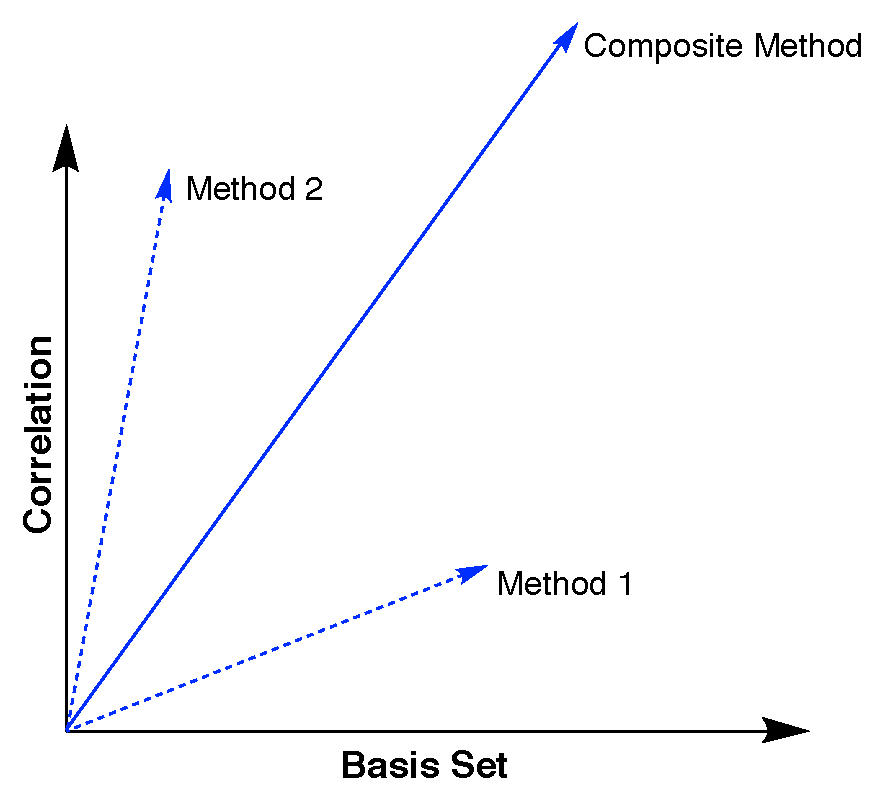
\includegraphics[height=20em]{figures/compositemethods.eps}
  \caption[Schematic representation of a quantum mechanical composite method.]{Schematic representation of a quantum mechanical composite method. The exact energy can only be achieved at the limits of an infinite basis set and complete correlation. Using a combination of Method 1 (low correlation/large basis set) and Method 2 (high correlation/small basis set), the Composite method approaches the exact energy.}
\label{fig:comp}
\end{figure}

\subsection{Density-functional theory}

Density-functional theory (DFT) is the most popular quantum chemical method applied to date. It relies on the two Hohenberg-Kohn theorems, the first of which states that there exists a unique electron density $\rho$ that defines the properties of a many-electron system. The second theorem defines an energy functional of the electron density and demonstrates that the correct ground state electron density minimises the energy functional through the variational theorem.\cite{Hohenberg1964,Koch2000} These theorems alone do not provide the solutions to the Schr{\"o}dinger equation.

It wasn't until the formulation of Kohn-Sham DFT\cite{Kohn1965} that the theory began gaining ground as a useful quantum theory. Kohn-Sham DFT scales formally with $N^3$ number of electrons\cite{Cramer2004} which is better than HF by a factor of $N$. In addition, DFT is a complete theory like FCI;\@ however, there is no straightforward way to determine the correct functionals of the electron density as the exact form of the functionals is unknown. Nonetheless, the drive for the development of the correct density-functional has been one of the main endeavours in quantum chemistry in the last two decades.

The framework behind conventional DFT is built into the description of the full energy functional $E$:

\begin{equation}
  E[\rho] = T_{ni}[\rho] + V_{ne}[\rho] + V_{ee}[\rho] + \Delta T[\rho] + \Delta V_{ee}[\rho]
\label{eq:DFT}
\end{equation}

\noindent where $T_{ni}$ is the kinetic energy of non-interacting electrons, $V_{ne}$ is the potential of nuclear-electron interactions, and $V_{ee}$ is the classical electron-electron repulsion. The last two terms are collectively referred to as the exchange-correlation (XC) functionals, where $\Delta T$ is the dynamical correlation term, and $\Delta V_{ee}$ is the non-classical correction to electron-electron repulsion. All the functionals, except the XC functionals have an exact form. It is therefore the XC functionals in which there is currently empiricism.

The ultimate goal in describing XC functionals is to find the ``correct'' XF functional which gives the exact energy of a system from the electron denisty. At this point, this must be done using approximations, for which there are several degrees of complexity. These approaches follow a hierarchical scheme, commonly referred to as the ``Jacob's ladder'' of DFT.\cite{Perdew2005} The first rung represents the simplest approximation which is known as local-density approximations (LDAs), which approximate the exchange-correlation density at a given point by the electron density at that same point. The form of these functionals is:

\begin{equation}
  E_{XC}^{LDA} = \int \rho (\mathbf{r}) \varepsilon_{XC} (\rho(\mathbf{r})) \mathrm{d}r
\end{equation}

\noindent where $\varepsilon_{XC}(\rho(\mathbf{r}))$ is the exchange-correlation energy per particle (energy density) of a uniform electron gas of density $\rho(\mathbf{r})$. This approximation is overly simple and applies only when the electron density if constant at all points, and are thus not generally applied in chemical problems. Nonetheless, LDA based approaches are commonly employed in solid state physics.

The second rung on the ladder corresponds to generalised-gradient approximation (GGA) based functionals, which are still amongst some of the most popular density-functionals. GGAs depend on both the electron density and the gradient of the electron density at a point:

\begin{equation}
  E_{XC}^{GGA} = \int \rho(\mathbf{r}) \varepsilon_{XC}^{GGA}(\rho(\mathbf{r}), \nabla \rho(\mathbf{r})) \mathrm{d}r
\end{equation}

\noindent where, $\varepsilon(\rho(\mathbf{r}), \nabla \rho(\mathbf{r})) \mathrm{d}r$ is the energy density associated with a given GGA.\@ GGA functionals provide a substantial improvement over LDAs, and most are constructed so that they correct the LDA energy:

\begin{equation}
  \varepsilon_{XC}^{GGA}(\rho(\mathbf{r}), \nabla \rho(\mathbf{r})) = \varepsilon_{XC}^{LDA}(\rho(\mathbf{r})) \mathrm{d}r + \Delta \varepsilon_{XC}\left( \frac{\nabla \rho(\mathbf{r})}{\rho^{4/3}({\mathbf{r}})}\right)
\end{equation}

A step above GGAs on the third rung of the ladder are meta-GGAs, which depend on the electron density, as well as the first derivative of electron density at a point, and the kinetic-energy density, $\tau(\mathbf{r})$, defined as:

\begin{equation}
  \tau(\mathbf{r}) = \sum_i^{occupied} \frac{1}{2}|\nabla \chi_i(\mathbf{r})|^2
\end{equation}

\noindent where $\chi_i(\mathbf{r})$ are the self-consistently determined Kohn-Sham orbitals. Meta-GGAs improve upon the accuracy of GGAs at a comparable cost.\cite{Cramer2004}

The XC functionals described up to this point (LDAs, GGAs, meta-GGAs) depend only on the electron density and derivatives of the electron density. The fourth and fifth rungs of the ladder improve upon the prior functionals by inclusion of terms dependent on additional properties. While this approach improves upon the accuracy of these functionals, it comes with an increase in computational cost. On the fourth rung sit functionals which depend to some percentage on the HF exact exchange. When the ratio of HF exchange is fixed, these functionals are termed hybrid functionals. Alternatively, functionals are said to be range-separated corrected if a different amount of exact-exchange to describe long and short-range behaviours. In the cases of hybrid and range-separated functionals, the added computational cost comes from the calculation of the HF exact exchange.

Alternatively, one can describe the fourth rung functionals as the depending upon the properties of the occupied molecular orbitals. The fifth rung then, is said to depend on the properties of unoccupied molecular orbitals. These functionals are typically referred to as double-hybrids, and incorporated correlation energy from a post-HF method, typically MP2.\cite{Goerigk2014} Double-hybrid DFT methods are once again more accurate than the lower rung methods, however, calculating the MP2 correlation energy is considerably more computationally demanding than traditional DFT approaches. Therefore, double-hybrid DFT methods have not gained popularity in the literature.

There are many published XC functionals. Fortunately, there is a fairly standard system of nomenclature, such that density functionals are described as \emph{exchange functional}-\emph{correlation functional}. The most commonly used density functional is the  B3-LYP, which uses the 3-parameter hybrid exchange functional of Becke,\cite{Becke1993} and the correlation functional of Lee, Yang, and Parr.\cite{Lee1988} There are also standalone functionals which have built in exchange and correlation functionals. A common example of these are the Minnesota family of functionals from the Truhlar group.\cite{Zhao2006,Zhao2006a}

Aside from the problem of choosing density-functionals, solving DFT is computationally very similar to the HF method. Within Kohn-Sham (KS) DFT, we define a fictitious system of non-interacting electrons with the same electron density as the real system. This is achieved by the use of a Hamiltonian in which there is an effective local potential, $V_s(\mathbf{r})$:

\begin{equation}
  \hat{H}_s = -\frac{1}{2}\sum_i^N\nabla_i^2 | \sum_i^N V_S(\mathbf{r}_i)
\end{equation}

\noindent The ground state wave function of this non-interacting Hamiltonian is represented by a single Slater determinant with spin orbitals ($\chi$), completely analogous to the HF problem. These spin orbitals, referred to as \emph{Kohn-Sham orbitals} are determined by

\begin{equation}
  \hat{h}_i^{KS} \chi_i = \varepsilon_i \chi_i
  \label{eq:kohnsham}
\end{equation}

\noindent where the one-electron Kohn-Sham operator $\hat{h}^{KS}$ is defined as

\begin{equation}
  \hat{h}_i^{KS} = -\frac{1}{2}\nabla^2 + V_s(\mathbf{r})
  \label{eq:ksoperator}
\end{equation}

It is crucial to realise that this procedure does not give us the exact energy of a system, but rather is used to determine an electron density which represents our real system. The connection between this fictitious system comes from the chose of the effective potential such that the density of our real system is a result of summing over the squared moduli of the KS orbitals:

\begin{equation}
  \rho(\mathbf{r}) = \sum_i | \chi_i |^2
\end{equation}

Once again in analogy to HF theory, on applies the variational principle to minimise the total energy functional in Equation~\ref{eq:DFT} with respect to $\chi$. The effective potential which variationally minimises the energy is given by\cite{Parr1995}

\begin{equation}
\begin{split}
  V_s(\mathbf{r}) &= \frac{\delta J[\rho]}{\rho(\mathbf{r})} + \frac{\delta E_{XC}[\rho]}{\delta \rho(\mathbf{r})} + \sum_A^M \frac{Z_A}{r_{iA}} \\
  &= \int\frac{\rho(\mathbf{r}_2)}{r_{12}} + V_{XC} + \sum_A^M \frac{Z_A}{r_{iA}}
\end{split}
\end{equation}

\noindent where the first term describes the Coulombic potential between two electrons, the last term is the potential between the electron and each nucleus. The middle term is once again the unknown XC potential. The electron density obtained from the fictitious system of non-interacting particles is finally used in Equation~\ref{eq:DFT} to find the total energy of the system. Since $V_s(\mathbf{r})$ depends on the electron density, these equation must be solvent iteratively, as with HF theory. Note however, that if the exact form of $E_{XC}[\rho]$ was known, this method would give the exact ground state electron density of the system, and thus the exact energy.

\subsubsection{Challenges for density-functional theory methods}

Pure DFT has low computational cost and potentially good accuracy, hence its popularity as a quantum chemical treatment. However, there are several problems which common DFT methods experience that lead to erroneous results in many cases.\cite{Cohen2012} It is well established that traditional DFT methods completely fail at describing non-covalent interactions.\cite{DiLabio2016} This shortcoming leads to poor descriptions of chemistry beyond equilibrium geometries, including transition states. Fortunately, there are several methods which can correct for this problem, commonly through the addition an energy correction term $E_{disp}$ to the DFT energy $E_{DFT}$, as

\begin{equation}
  E_{tot} = E_{DFT} + E_{disp}
\end{equation}

\noindent It is common to employ the empirical D3 pair-wise correction of Grimme,\cite{Grimme2010} paired with of the Becke-Johnson damping functions,\cite{Johnson2006} denoted as D3(BJ). This correction works by calculating the dispersion interactions between all pairs of atoms $A$ and $B$ separated by distance $R_{AB}$, with the following equation:

\begin{equation}
  E_{disp} - \sum_{A>B} \frac{C_6^{AB}}{R_{AB}^6} f_6(R_{AB}) + s_8
  \frac{C_8^{AB}}{R_{AB}^8} f_8(R_{AB})
\end{equation}

\noindent where $C_6$ and $C_8$ are dispersion coefficients, $s_8$ is an empirically determined scaling parameter, and $f_n$ are the damping functions which limit the range of dispersion correction, avoiding near singularities at small $R_{AB}$. Another approach to correcting for dispersion is to add parameters directly to the functional, as is the case in the Minnesota functionals.\cite{Zhao2006,Zhao2006} Both of these empirical corrections have the benefit of adding negligible computational time, but must be parametrised for each DFT method with which they are employed.

Another striking issue with DFT is the unphysical ability of an electron to interact with itself, termed \emph{self-interaction error}. This is most obvious in what is known as \emph{delocalisation error}, which is a result of many-electrons interacting with themselves, or many-electron self-interaction error. In HF theory, self-interaction error is exactly cancelled, thus DFT methods which have a high portion of HF exchange in their formulation are able to account for this issue. Consider for a moment a one electron system: there should be exactly zero electron correlation. In terms of the energy functionals shown in Equation~\ref{eq:DFT}, the electronic repulsion term $V_{ee}[\rho]$ should cancel exactly with the XC term ($V_{ee}[\rho] = -E_{XC}[\rho]$).\cite{Cramer2004} Unfortunately, all pure DFT methods fail to reproduce this expected behaviour. An obvious manifestation of delocalisation error is the incorrect treatment of charge-transfer in intramolecular interactions,\cite{MoriSanchez2008,OterodelaRoza2014} as well as in transition state complexes. Even for the simplest HAT reaction \ch{H2 + H^. -> H^. + H2}, the calculated barrier height is underestimated by 8--9 \kcalmol using a GGA functional.\cite{Csonka1998} Charge-transfer occurs when a fraction of an electron is transferred between molecular entities. Specifically, charge-transfer is mistreated at longer ranges, thus either high percentage exact exchange hybrid functionals, or range-separated functionals are suggested for systems in which charge-transfer may occur.

As is the case for most experimental methods, identifying the correct theoretical methods requires the careful consideration of the problem at hand. Choosing a DFT based method requires calibration, however, once a method has been tested and is known to provide reasonably accurate results, DFT methods have the ability to help understand chemical problem with relatively low computational costs.

\section{Applying theory to chemical problems}

\subsection{Geometry optimisation}

All QM methods depend parametrically on the geometry of a molecular system. That is the electronic energy of a system depends on the positions of the nuclei. While the wave functions can describe any arbitrary geometry, we are typically only interested in certain geometries of a molecule. These geometries of interest are normally stationary states along a the potential energy surface (PES) of a system, that is, points where the gradient of energy with respect to nuclear coordinates is zero. Therefore, we perform \emph{geometry optimisation} calculations to determine these points.

Molecular systems have complex PESs. For a non-linear molecule, the nuclear PES has 3$N$-6 dimensions, where $N$ is the number of nuclei present.\cite{Heidrich1991} In geometry optimisation, we seek the local minima (reactants, products, or intermediates) and local maxima (TS complexes). Consider only local minima for a moment. Often complex molecules have more than one possible conformation, and each conformation represents a different local minimum along the PES.\@ It is therefore important to ensure the correct conformation, typically the lowest energy structure (global minimum), is used when approaching chemical problems.

In order to efficiently perform geometry optimisation, numerical analysis techniques are employed. All geometry optimisation methods follow the same general framework.\cite{Hratchian2005} First, energy and necessary derivatives are computed from an initial geometry. Second, the geometry is modified to step towards the nearest stationary state. And last, some test is performed to determine if the new geometry is near enough to the stationary state along the PES.\@ The most efficient method to do this is the \emph{Newton method}, in which the energy is expanded in a Taylor series (truncated at the second order point) about the current point, $\mathbf{x}_0$:

\begin{equation}
  E(\mathbf{x}) = E_0 + \mathbf{g}_0\Delta\mathbf{x} + \frac{1}{2}\Delta\mathbf{x}\mathbf{H}_0\Delta \mathbf{x}
\end{equation}

\noindent where $E_0$, $\mathbf{g}_0$, and $\mathbf{H}_0$ are the energy, gradient (Jacobian), and second derivative (Hessian) at point $\mathbf{x}_0$, and $\Delta \mathbf{x} = x_i - x_0$. The aim of the Newton method is to minimise the gradient of the Taylor expansion, $\mathbf{g(x)}$, such that

\begin{equation}
  \mathbf{g(x)} = \mathbf{g}_0 + \mathbf{H}_0 \Delta \mathbf{x}
\end{equation}

\noindent Solving for $\Delta \mathbf{x}$ gives the so-called Newton step that leads to minimisation:

\begin{equation}
  \Delta \mathbf{x} = -\mathbf{H}^{-1}_0\mathbf{g}_0
\end{equation}

The analytic computation of the Hessian is very expensive, especially for large systems. Therefore, to simply the problem at the beginning of geometry optimisation, the Hessian matrix is approximated and updated at each step in the optimisation, using clever algorithms.\cite{Hratchian2005} This is called the \emph{quasi-Newton method}, and is the default optimisation routine in the Gaussian\cite{Frisch2009} quantum chemistry package, as well as many other quantum chemistry packages.

Some additional caution must be taken in optimising molecular structures. Normal algorithms which optimise structures stop when the gradient of energy is sufficiently close to zero; however, often PES can be flat or very shallow in regions and structures that are not fully optimised can be obtained. To avoid this, geometries are always subject to molecular vibration analysis.

\subsection{Molecular vibrations}

The computation of molecular vibrations can be performed simply given a set of molecular coordinates.\cite{Wilson1980} Assuming a non-linear molecule, we start with 3$N$-6 internal coordinates which are non-coupled (orthogonal). We then apply the \emph{harmonic approximation}, in which we assume each normal mode follows Hooke's Law

\begin{equation}
  F = kx
\end{equation}


\noindent where $F$ is the force, $k$ is the force constant, and $x$ is the displacement along one normal mode's coordinates. This approximation assumes the PES along the normal mode is parabolic, which in general is not true, but is a good approximation near the minima. Deviations from this approximation are known as \emph{anharmonicity}. In practise, however, at normal temperatures ($\sim$ 298K) the harmonic approximation is sufficient to describe molecular vibrations as displacements are assumed to be small.

Typically to obtain molecular frequencies, one computes the mass-weighted Hessian matrix elements $F_{ij}$

\begin{equation}
  F_{ij} = \frac{1}{\sqrt{m_i m_j}} \mathbf{H}_{ij}
\end{equation}

\noindent where the partial derivatives of internal coordinates $x_i$ of the potential energy $U$ are taken for 3$N$ atoms with mass $m$. One then seeks to diagonalise this $3N\times3N$ matrix to obtain eigenvalues $\lambda_i$, which describe the force constant of each normal mode. The harmonic frequencies $\nu_i$ are then obtained by

\begin{equation}
  \nu_i = \frac{\sqrt{\lambda_i}}{2\pi}
\end{equation}

\noindent and the lowest 6 modes are then discarded to account for 3$N$-6 normal modes. These lowest energy modes generally correspond the internal rotations, and thus must be discarded to correctly obtain thermochemical corrections.

From these frequencies, the \emph{zero-point vibrational energy} (ZPE, $E_{ZPE}$) is calculated:

\begin{equation}
  E_{ZPE} = \sum_{i=1}^{3N-6} \frac{h\nu_i}{2}
\end{equation}

\noindent The ZPE is an important quantum correction to the classical potential, giving the electronic potential energy

\begin{equation}
U = E_{elec} + E_{ZPE}
\end{equation}

\noindent where $E_{elec}$ is the QM electronic energy.

If a normal mode describes a non-minimum along the PES, the energy gradient will be negative (imaginary) instead of positive. Only energy maxima or saddle-points (TS structures) should have a single imaginary mode. Therefore, if a non-TS molecular structure calculation yields one or more imaginary modes, the geometry optimisation has yielded a structure which is not at minimum on the PES.\@ In this situation additional steps must be taken to find a corrected structure.

\subsection{Thermochemistry}

Up until this point we have been viewing molecules from a microscopic perspective; however, this is not useful for describing properties of bulk systems. Fortunately, fundamental statistical thermodynamics can be used to approximately describe a system in bulk.\cite{McQuarrie1999,McQuarrie2000} We approximate our system as an ensemble of non-interacting particles: the ideal gas. Within statistical thermodynamics, the fundamental starting point is the partition function $Q$,\cite{note4} from which all thermodynamic properties can be calculated. For our ensemble, the molecular partition function is

\begin{equation}
  Q = \sum_J e^{\varepsilon_j/k_B T}
\end{equation}

\noindent where a Boltzmann distribution of $j$ energy states $\varepsilon$ is taken at temperature $T$, and $k_B$ is the Boltzmann constant. All calculations herein are defined under conditions of temperature $T$ = 298.15 K and pressure $P$ = 1 atm.

Normally, the molecular partition function is decomposed into contributions from translational, vibrational, rotational, and electronic motion:

\begin{equation}
  Q = q_{trans}q_{vib}q_{rot}q_{elec}
\end{equation}

\noindent The equation describing the translational partition function
$q_{trans}$ is

\begin{equation}
  q_{trans} = \left( \frac{2\pi m k_B T}{h^2} \right)^{3/2} \frac{k_B T}{P}
\end{equation}

\noindent where $m$ is the mass of the molecule, $h$ is Planck's constants.

The vibrational partition function $q_{vib}$ depends on the contributions of each of $K$ vibrational modes. Only the $3N-6$ (or $3N-5$ for linear molecules) real vibrational modes of a molecule are considered, and imaginary frequencies are ignored. Therefore, for molecules which posses an imaginary frequency this thermodynamic analysis is invalid. TS complexes do posses a single imaginary frequency which is ignored, as it is assumed to not contribute to the overall vibrational partition function as no formal bond is said to be formed in the acceptor-donor system. Each vibrational mode has a characteristic vibrational electronic temperature, $\Theta_{\nu,K} = h\nu/k_B$, and the partition function is

\begin{equation}
  q_{vib} = \prod_K \frac{e^{-\Theta_{\nu,K}/2T}}{1 - e^{-\Theta_{\nu,K}/T}}
\end{equation}

The rotational partition function depends on the geometry of a system. For a single molecule $q_{rot}$=1. For a linear molecule, the rotational partition function is

\begin{equation}
  q_{rot} = \frac{1}{\sigma_r} \left(\frac{T}{\Theta_r}\right)
\end{equation}

\noindent where $\sigma_r$ is the symmetry number for rotation which depends on the molecular symmetry, and $\Theta_r = h^2/8\pi^2Ik_B$. $I$ is the moment of inertia. Finally, for a non-linear polyatomic molecule, the rotational partition function is

\begin{equation}
  q_{rot} = \frac{\sqrt{\pi}}{\sigma_r}\left(\frac{T^{3/2}}{\sqrt{\Theta_{r,x}\Theta_{r,y}\Theta_{r,z}}}\right)
\end{equation}

\noindent where $\Theta_{r,x}, \Theta_{r,y}$, and $\Theta_{r,z}$ describe contributions of the moment of inertia in each of the x, y, and z-planes.

Finally, we make an important assumption that electronic contributions are assumed to exist in only the ground state, as excited states are generally safely assumed to be much larger than $k_B T$ in energy. The full electronic partition function is

\begin{equation}
  q_{elec} = \sum_{i=0} \omega_i e^{-\epsilon_i/k_B T}
\end{equation}

\noindent where $\omega$ is the degeneracy of an energy level with energy $\epsilon$. Applying our assumption, and by setting the ground state energy $\epsilon_0=0$, our problem simplifies dramatically, such that $q_{elec} = \omega_0$, which is simply the spin multiplicity of the molecule.

We now have all the information needed to calculate the thermodynamic quantities we are interested in. In chemistry we are concerned with the Gibbs free energy $G$, which is defined by the entropy $S$ and enthalpy $H$ as

\begin{equation}
  G = H - TS
\end{equation}

\noindent From each of the partition functions, the entropy of a system with $N$ moles, $S_{tot} = S_{trans} + S_{vib } +S_{rot} + S_{elec}$, is calculated using the relation

\begin{equation}
  S = Nk_B + Nk_B\ln\left( \frac{Q}{N} \right) + Nk_B T \left( \frac{\partial
      \ln Q}{\partial T} \right)_V
\end{equation}

\noindent Similarly, the internal energy of a system, $E_{int,tot} = E_{int,trans} + E_{int,vib} + E_{int,rot} + E_{int,elec}$, is given by the relation

\begin{equation}
  E_{int} = Nk_B T^2\left( \frac{\partial \ln Q}{\partial T} \right)_V
\end{equation}

\noindent Finally, the enthalpy is obtained from

\begin{equation}
  H_{tot} = E_{int,tot} + k_B T
\end{equation}

Using very simple statistical thermodynamic arguments, the properties of a bulk system are easily computed. It is important to emphasise that these results are for particles in the gas phase, thus additional steps must be taken if one desires to compare results to experiments performed in solvent.

\subsection{Modelling solvent}

It is in principle possible to include solvent molecules explicitly in QM calculations: this is in practise, extremely cost prohibitive. In order to approximate the important contributions of solvation, so-called \emph{implicit continuum solvent models} are generally employed.\cite{Mennucci2007,Cramer2004} Mathematically, one describes this as

\begin{equation}
  \hat{H}^{tot}(\mathbf{r}_m) = \hat{H}^{mol}(\mathbf{r}_m) + \hat{V}^{mol+sol}(\mathbf{r}_m)
\end{equation}

\noindent where a perturbation $\hat{V}^{mol+sol}$ dependent only on the coordinates of the solute ($\mathbf{r}_m$; thus implicit) is applied to the Hamiltonian of the solute. The perturbation term is composed of interaction operators which contribute to the net free energy:

\begin{equation}
G_{solv} = G_{cavity} + G_{electrostatic} + G_{dispersion} + G_{repulsion} +
G_{solv~kinetic}
\end{equation}

\noindent where the total solvation free energy $G_{solv}$ contains terms from: the formation of a solvation cavity $G_{cavity}$, the electrostatic interactions between solvent and solute $G_{electrostatic}$, the dispersion interactions between solvent and solute $G_{dispersion}$, the QM exchange repulsion between solvent and solute $G_{repulsion}$, and the movement of solvent molecules $G_{solv~kinetic}$.

A widely used model for solvation comes from the Truhlar group, and is known as SMD.\cite{Marenich2009} The main parameter in implicit solvent models is the solvent dielectric constant ($\varepsilon$) with contributions from surface tension and the solvent-solute interface. SMD also includes terms which depend on the electron density of the solute.  While many other implicit solvent models require the use of the same QM method as they were parametrised,\cite{Ho2010} SMD is a \emph{universal} model which was parametrised using several QM methods. Therefore, it does not require the use of a specific QM method and can be applied broadly in both single point energy and geometry optimisation calculations.

\subsection{Rate constants and transition state theory}

In the discussion of chemical kinetics, the rate ($r$) of a bimolecular reaction

\begin{equation}
  \ch{$a$ A + $b$ B <=> $c$ C + $d$ D}
  \label{eq:a}
\end{equation}

\noindent is determined by the \emph{rate law}, which can generally be described as

\begin{equation}
  r = \frac{d \text{C}}{dt} =\frac{d \text{D}}{dt} = k[A]^a [B]^b
\end{equation}

\noindent where $k$ is the rate constant, $t$ is time, $A, B, C$, and $D$ are chemical species with stoichiometric coefficients $a, b, c$, and $d$, and $k$ is the rate constant. Computational chemistry is in general, not useful for determining rate laws: this must be done experimentally. Where computational studies can be useful, is in determining reaction mechanisms, and how the reaction barrier height can be altered. In doing so, we focus entirely on $k$.

Most chemists are intimately familiar with the phenomenological \emph{Arrhenius equation}

\begin{equation}
  k_{Arr} = Ae^{-E_a/RT}
\label{eq:arrhenius}
\end{equation}

\noindent where $A$ is a constant, $R$ is the gas constant, and $E_a$ is the \emph{activation energy}, which is an experimental measure of the reaction barrier height. This equation dates back to the 1880s, when Arrhenius noticed that the reactions depended more heavily on temperature than was intuitive, and thus introduced the $A$ constant, known often as the Arrhenius pre-factor.\cite{McQuarrie1997} The Arrhenius pre-factor is an empirical measure of how factors other than kinetic energy affect the rate constant. From the perspective of theory, Equation~\ref{eq:arrhenius} has little meaning as the parameters are empirical. Thus, to study rate constants theoretically we must turn to \emph{transition state theory}.

\subsubsection{Transition state theory}

The study of transition state theory (TST) originates in the 1930s, and was developed primarily by Eyring.\cite{McQuarrie1997,Steinfeld1998} In TST we focus on the TS complex, which is defined as a transient species which exists at the top of the energy barrier of a reaction. If we consider the same reaction in Equation~\ref{eq:a}, and set all the coefficients to 1, then TST states the reaction proceeds in two steps, the first of which includes a quasi-equilibrium between the reactants and TS complex

\begin{equation}
  \ch{A + B <=>AB$^\ddagger$ <=> C + D}
  \label{eq:tst}
\end{equation}

\noindent with an equilibrium constant ($K_c^{\ddagger}$) expression

\begin{equation}
  K_c^{\ddagger} = \frac{[\ch{AB}^\ddagger]/c^0}{[\ch{A}]/c^0[\ch{B}]/c^0}
\label{eq:K}
\end{equation}

\noindent where $c^0$ is the standard-state concentration (normally taken to be 1 M).

\begin{figure}[htb]
    \centering
    \includegraphics[width=0.6\textwidth]{figures/TST-PES.png}
    \caption[A reaction coordinate diagram for a generic reaction.]{A reaction coordinate diagram for the reaction of Equation~\ref{eq:tst}. The TS complex is defined to exist in the small region $\delta$ above the reaction barrier.}
\label{fig:tst-pes}
\end{figure}

In TST, we define the TS complex to exist throughout a small region of width $\delta$ above the reaction barrier (\ref{fig:tst-pes}). From the second step of the reaction in Equation~\ref{eq:tst}, we can define a reaction rate dependent on the concentration $[\ch{AB}^\ddagger]$ and $v_c$, a factor which defines the frequency with which the complexes proceed over the barrier:

\begin{equation}
  r = v_c [\ch{AB}^\ddagger]
\end{equation}

From Equations~\ref{eq:a} and~\ref{eq:tst}, we now have two equivalent expressions for the reaction rate, which allows us to derive the following

\begin{equation}
  r = k[\ch{A}][\ch{B}] = v_c [\ch{AB}^\ddagger]
\end{equation}

\noindent and solving Equation~\ref{eq:K} for $[\ch{AB}^\ddagger]$ results in


\begin{equation}
  r = v_c\frac{[\ch{A}][\ch{B}]K_c^\ddagger}{c^0}
\end{equation}

\noindent or

\begin{equation}
  k = \frac{v_c K_c^\ddagger}{c^0}
\label{eq:b}
\end{equation}

We must now invoke the statistical thermodynamics to make sense of Equation~\ref{eq:b}. We can rewrite the equilibrium expression $K_c^\ddagger$ in terms of partition functions of each molecular species:

\begin{equation}
    K_c^{\ddagger} = \frac{[\ch{AB}^\ddagger]/c^0}{[\ch{A}]/c^0[\ch{B}]/c^0}
    = \frac{(q^\ddagger/V)c^0}{(q_A/V)(q_b/V)}
\label{eq:c}
\end{equation}

\noindent where $V$ is the volume, and $q_A$, $q_B$, and $q^\ddagger$ are the partition functions of A, B, and AB$^\ddagger$, respectively.

Since we have defined the reaction to be occurring with one degree of freedom, the translational partition function $q_{trans}$ can be defined as

\begin{equation}
  q_{trans} = \frac{\sqrt{2\pi m^\ddagger k_B T}}{h}\delta
\end{equation}

\noindent where $m^\ddagger$ is the mass of the TS complex. The partion function of the TS complex can be written as the product $q^\ddagger = q_{trans}q_{int}^\ddagger$, where the second term accounts for all remaining degrees of freedom of the TS complex. We can use this and rewrite Equations~\ref{eq:c} and~\ref{eq:b} as

\begin{equation}
  K_c^{\ddagger} =  \frac{\sqrt{2\pi m^\ddagger k_B T}}{h}\delta\frac{(q_{int}^\ddagger/V)c^0}{(q_A/V)(q_b/V)}
\end{equation}

\noindent and

\begin{equation}
 k = v_c \frac{\sqrt{2\pi m^\ddagger
     k_B T}}{hc^0}\delta\frac{(q_{int}^\ddagger/V)c^0}{(q_A/V)(q_b/V)}
\label{eq:d}
\end{equation}

We are now left with the two terms $v_c$ and $\delta$ which are ill-defined. However, the product of these two terms is the average speed at which the TS complex crosses the barrier, $\langle u_{TS} \rangle = v_c\delta$. A Maxwell-Boltzmann distribution is used to calculate the value of $\langle u_{TS} \rangle$:

\begin{equation}
  \langle u_{TS} \rangle = \left( \frac{m^\ddagger}{2\pi k_B T} \right)^{1/2}
  \int_0^\infty u e^{-m^\ddagger u^2/2k_B T}du = \left( \frac{m^\ddagger}{2\pi
      k_B T m^\ddagger} \right)^{1/2}
\label{eq:e}
\end{equation}

\noindent Substituting Equation \ref{eq:e} into Equation~\ref{eq:d} for $v_c\delta$ yields

\begin{equation}
  k =
  \frac{\sqrt{k_B T}}{hc^0}\frac{(q_{int}^\ddagger/V)c^0}{(q_A/V)(q_b/V)} = \frac{k_B T}{hc^0}K_c^\ddagger
\label{eq:f}
\end{equation}

Now, define the standard Gibbs free energy of activation ($\Delta ^\ddagger G^0$) to be the change in Gibbs free energy in going from reactants to TS.\@ The thermodynamical expression is

\begin{equation}
  \Delta ^\ddagger G^0 = -RT \ln K_c^\ddagger
\end{equation}

\noindent which can be substituted into Equation~\ref{eq:f}

\begin{equation}
  k = \frac{k_B T}{hc^0} e^{-\Delta^\ddagger G^0/RT}
\label{eq:g}
\end{equation}

The standard Gibbs free energy of activation can be expressed in terms of enthalpy and entropy as

\begin{equation}
  \Delta^\ddagger G^0 = \Delta^\ddagger H^0 - T \Delta^\ddagger S^0
\end{equation}

\noindent which, upon substitution gives the equation

\begin{equation}
  k = \frac{k_B T}{hc^0} e^{-\Delta^\ddagger S^0/R} e^{-\Delta^\ddagger H^0/RT}
\label{eq:M}
\end{equation}

At this point, we can draw a direct comparison to the Arrhenius equation (Equation~\ref{eq:arrhenius}) by expressing $E_a$ in terms of $\Delta^\ddagger H^0$ and $A$ in terms of $\Delta^\ddagger S^0$.  We must differentiate the natural logarithm of Equation~\ref{eq:f}, as well as Equation~\ref{eq:arrhenius} (assuming that $A$ is independent of temperature):

\begin{equation}
  \frac{d \ln k}{dT} = \frac{1}{T} + \frac{d \ln K_c^\ddagger}{dT}
  \label{eq:h}
\end{equation}

\begin{equation}
  \frac{d \ln k_{Arr}}{dT} = \frac{E_a}{RT^2}
  \label{eq:i}
\end{equation}

\noindent Next, we use the fact that $d \ln K_c / dT = \Delta U^0/RT^2$ for an ideal gas, then Equation \ref{eq:h}  becomes

\begin{equation}
  \frac{d \ln k}{dT} = \frac{1}{T} + \frac{\Delta ^\ddagger U^0}{RT^2}
  \label{eq:j}
\end{equation}

\noindent Additionally, $\Delta ^\ddagger H^0 = \Delta ^\ddagger U^0 + RT \Delta^\ddagger n$ ($\Delta^\ddagger n = 1$), as so Equation~\ref{eq:j} can be rewritten as

\begin{equation}
  \frac{d \ln k}{dT} = \frac{\Delta ^\ddagger H^0 + 2RT}{RT^2}
  \label{eq:k}
\end{equation}

\noindent Therefore, by comparison of Equation~\ref{eq:k} and \ref{eq:i}, we get

\begin{equation}
  E_a = \Delta^\ddagger H^0 + 2RT
\end{equation}

\noindent which then converts Equation~\ref{eq:M} into the form

\begin{equation}
  k = \frac{e^2k_B T}{hc^0}e^{\Delta^\ddagger S^0/R}e^{-E_a/RT}
\end{equation}

Therefore, a statistical thermodynamical picture of the Arrhenius equation arises from TST, and the Arrhenius pre-factor $A$ can be expressed as

\begin{equation}
  A = \frac{e^2k_B T}{hc^0}e^{\Delta^\ddagger S^0/R}
\label{eq:afactor}
\end{equation}

In practise, we use the form of Equation~\ref{eq:g} to compute the rate constant of a reaction, which we shall denote as $k_{TST}$. The conventional TST makes an assumption that the reaction coordinate is static along the lowest energy pathway. This can be corrected by the use of \emph{variational transition state theory}.\cite{Truhlar1984} We shall not consider variational TST in this work, as with careful application, conventional TST does a remarkably good job at accounting for the magnitude and temperature dependence of a wide range of reactions.\cite{Steinfeld1998} Additionally, if one makes corrections for \emph{QM tunnelling}, conventional TST can easily give a more complete description of the rate constant.

\subsubsection{Quantum mechanical tunnelling}

Atoms are quantum mechanical particles, and are thus subject to the strange probabilistic behaviours observed at the microscopic level. QM tunnelling refers to the ability of particles to penetrate the reaction barrier, rather than surmounting it classically (\ref{fig:tunnelling}). While all reactions are subject to QM tunnelling, we will show that due to the low mass of the hydrogen atom, QM tunnelling can play a significant role in HAT reactions.

\begin{figure}[htb]
  \centering
  \includegraphics[width=0.5\textwidth]{figures/tunnelling-1}
  \caption{Quantum mechanical tunnelling occurs when a particle penetrates a
    reaction barrier, rather than surmounting it. Figure adapted from Reference~\citenum{McMahon2003}.}
\label{fig:tunnelling}
\end{figure}


In order to determine the effects of scattering, one must find transmission coefficients ($\kappa$) by solving the Schr{\"o}dinger equation.\cite{Griffiths2016} This is done by approximating the reaction barrier with an analytical potential, thus simplifying the problem mathematically. The earliest model potentials were introduced by Bell, who used a parabolic function to approximate the reaction barrier.\cite{Bell1980} To obtain $\kappa$, and thus the observed rate constant ($k_{obs}$), the following equations were used:

\begin{align}
  k_{obs} &= \kappa A e^{-E_a/RT}  \\
\kappa &= \frac{e^\alpha}{\beta-\alpha} \left(\beta e^{-\alpha} - \alpha
  e^{-\beta} \right) \\
  \alpha &= E_a/RT \\
  \beta &= \frac{2a\pi^2(2mE_a)^{1/2}}{h}
\end{align}

\noindent where the Arrhenius equation was used to estimate the rate constant, $m$ is the mass of the tunnelling particle, and $2a$ is the width of the barrier. Since the equation is dependent on the mass of the particle, tunnelling occurs more often when lighter particles are involved. As a consequence, tunnelling is more common in HAT reactions than other atom transfer reactions. Also, the height and width of the barrier are important factors in determining the contributions to tunnelling: reactions with small barriers have low tunnelling contributions; narrow barriers result in higher tunnelling contributions.

The Bell model is a poor representation of an actual reaction barrier. One which is a much better approximation is the \emph{Eckart potential}.\cite{Johnston1962} The form of this potential is

\begin{align}
  V &= -\frac{Ay}{1-y} - \frac{By}{1-y^2} \\
  y &= -e^{2\pi x/L}
\end{align}

\noindent where $x$ is the variable along the reaction coordinate and $L$ is called the characteristic length. If $A=0$ the potential becomes a symmetric function, further simplifying the problem; however, most reactions do not have a symmetric potential. $A$, $B$ and $L$ are related to the change in barrier height in the forward and reverse direction, $\Delta V_1$ and $\Delta V_2$, respectively:

\begin{align}
  A &= \Delta V_1 - \Delta V_2 \\
  B &= ((\Delta V_1)^{1/2} + (\Delta V_2)^{1/2})^2 \\
 \frac{L}{2\pi} &= (-\frac{2}{F^*})^{1/2} [\frac{1}{(\Delta V_1)^{1/2}} +
      \frac{1}{(\Delta V_2)^{1/2}}]^{-1}
\end{align}

\noindent where $F^* = d^2V/dx^2$ evaluated at the maximum of the potential. In this formulation, $V$ is a placeholder energy. Note that if a reaction is endoergic, tunnelling does not occur. Alternatively, one says tunnelling only occurs in exoergic or energy-neutral reactions.

The solutions to the Schr{\"o}dinger equation for the Eckart potential are analytical, thus that transmission coefficient $\kappa$ can easily be computed using standard numerical techniques. These tunnelling corrections will be applied, where applicable as

\begin{equation}
  k_{calc} = \kappa k_{TST} = \kappa
\frac{k_B T}{hc^0}e^{-\Delta^\ddagger G^0}
\end{equation}


%%\chapter{Methods}
\label{ch:methods}

%%% Local Variables:
%%% mode: latex
%%% TeX-master: "diss"
%%% End:


% !TEX root = diss.tex

\chapter{The Relationship Between Arrhenius Pre-factors with Non-Covalent Binding}
\label{ch:arrhenius}

\begin{doublespace}
\section{Introduction}

DiLabio and Ingold\cite{DiLabio2005} previously investigated the formal HAT
reaction of the iminoxyl/oxime self-exchange reaction. In that paper, they
compiled a table of parameters from the phenomenological Arrhenius equation for
a series of interesting reactions, which appear here
in~\ref{tab:Arrhenius-expt}.\cite{Kreilick1966, Mader2004, Mahoney1970,
DaRooge1967, Howard1973, Foti1994, Chenier1974, Chenier1975} These are
thermoneutral hydrogen atom self-exchange reactions involving oxygen-centered
radicals, and other nearly thermoneutral reactions involving the destruction and
formation of oxygen-centered radicals, reactions 3.1 and 3.2, respectively:

\begin{align}
  \ch{$\pi$-RO^. + ROH &-> ROH + $\pi$-RO^.} \hspace{2cm} \Delta H = 0 \\
  \ch{$\pi$-R}^\prime\ch{O^. + ROH &-> R}^\prime\ch{OH + $\pi$-RO^.} \hspace{2cm} \Delta H \approx 0
\end{align}

\newcommand{\tabFig}[2][0.35]{\includegraphics[scale=#1]{figures/#2.eps}}

\begin{table}[!ht]
  \footnotesize
  \centering
  \caption[Table of results for (nearly) thermoneutral reactions
  studied.]{Table of results for (nearly) thermoneutral reactions studied. Units
  for $\Delta H$, $E_a$, and calculated pre-reaction complex binding energy (BE)
  are \kcalmol, $\log A$ are log \Ms, and $k$ are \Ms.\ References to the
  original literature are included with the Complex ID number.
  $^\dagger$Calculated binding energies involve structures that could not be
  fully optimized and contain one or more small imaginary frequencies. Adapted
  with permission from Reference \protect\citenum{DiLabio2005}. Copyright (2005)
  American Chemical Society.}
  \begin{tabular}{l >{\centering}m{1.5cm} >{\centering}m{1.5cm}
  >{\centering}m{1.3cm} >{\centering}m{1.3cm} >{\centering}m{1.3cm}
  >{\centering}m{1.3cm} >{\centering}m{1.3cm} m{0em}}
  ID & \ch{RO^.}/\ch{R}$^\prime$\ch{O^.} & \ch{ROH} & $\Delta H$ & $\log~A$ & $E_a$ & $k$ & BE & \\
  \toprule
  1\cite{Kreilick1966} & \tabFig{3tBuPhO} & \tabFig{3tBuPhOH} & 0.0 & 3.7 & 1.2 & 3.3\E{2} & -10.8 &\\
  2\cite{Mader2004} & \tabFig{4MeC5H4ONO} & \tabFig{4MeC5H6NOH} & -2.0 & 3.8 & 3.8 & 10 & -14.8 &\\
  3\cite{Kreilick1966}& \tabFig[0.4]{2tBuNO} & \tabFig[0.4]{2tBuNOH} & 0.0 & 5.1 & 3.5 & 3.3\E{2} & -10.1$^\dagger$ &\\
  4\cite{Mahoney1970,DaRooge1967} & \tabFig{3tBuPhO} & \tabFig{tBuPhOH} & 4.2 & 5.5 & 4.8 & 93 & -10.0$^\dagger$ &\\
  5\cite{Howard1973} & \tabFig[0.7]{tBuOO} & \tabFig{3tBuPhOH} & -7.0 & 4.2 & 0.5 & 7\E{3} & -6.5 &\\
  6\cite{Kreilick1966} & \tabFig[0.7]{Ph2NO} & \tabFig[0.7]{Ph2NOH} & 0.0 & $>$7 & - & $>$10$^7$ & -13.6$^\dagger$ &\\
  7\cite{Foti1994} & \tabFig{PhO} & \tabFig{2hydroxynaphthalene} & -2.2 & 8.3 & 2.3 & 4\E{6} & -8.6 &\\
  8\cite{Chenier1974} & \tabFig[0.7]{tBuOO} & \tabFig{PhOH} & 0.3 & 7.2 & 5.2 & 3\E{3} & -5.5$^\dagger$ &\\
  9\cite{Chenier1974} & \tabFig[0.7]{tBuOO} & \tabFig{2hydroxynaphthalene} & -1.9 & 6.4 & 2.6 & 3\E{4} & -5.6$^\dagger$ &\\
  10\cite{Chenier1975} & \tabFig[0.7]{tBuOO} & \tabFig{alphatetralinperoxide} & 1.4 & 6.0 & 4.5 & 7\E{2} & -8.0$^\dagger$ &
\end{tabular}
\label{tab:Arrhenius-expt}
\end{table}

Although it is well known that reactions of this nature involve remarkably low
activation energies ($E_a$),\cite{Lucarini1996, Mahoney1970a, Mahoney1975,
Korcek1972} the Arrhenius pre-exponential factors ($A$), or as they shall be
referred to herein, \emph{A-factors}, as a well as rate constants, span a wide
range (summarized in~\ref{tab:Arrhenius-expt}): The measured A-factors range
from $10^{3.5}$--$10^{8.3}$ \Ms\ and the rate constants range from 10--10\E{7}
\Ms.\ In the past, this range has been attributed to steric shielding around the
oxygen atoms, resulting in a larger entropic barriers.\cite{DiLabio2005}
Importantly, it was noted that the degree of steric shielding on the oxygen atom
appears to play an important role in the order of the A-factor; systems with
greater bulk have lower A-factors, while non-shielded systems have larger
A-factors.

Stereo-electronic effects are known to play an important role in HAT, and have
been studied extensively.\cite{Finn2004, Salamone2011, Pischel2001, Griller1981,
Bietti2011, Salamone2012, Malatesta1982, Salamone2014} Although the abstraction
of a specific hydrogen atom may be more thermodynamically favourable than others
on a given substrate, if it is not accessible due to steric constraints,
abstraction will not occur at this site. Otherwise, additional steric bulk can
lead to significant reductions in reactivity, through destabilization of the TS
complex, or by forcing additional processes involving conformational changes in
order to reach the appropriate TS structure. For example, in reactions of
tertiary acetamides with \cumo,\cite{Salamone2014} where abstraction occurs
mainly from C-H bonds $\alpha$ to the nitrogen atom, a two-fold decrease in the
rate constant (normalized for the number of equivalent hydrogen atoms) is
observed in going from $N,N$-dimethylacetamide to $N,N$-diisobutylacetamide
($k_H$ = $2.0 \times 10^5$ and $7.8 \times 10^4$ \Ms, respectively). The
decrease in rate constant is attributed to the steric clash between the methyl
groups of \cumo\ and the isobutyl groups of $N,N$-diisobutylacetamide.

As all of the reactions in~\ref{tab:Arrhenius-expt} are nearly thermoneutral,
thermochemical effects on the rates of reaction are expected to be minimal.
Therefore, the large degree of variance in their rate constants ($k$) is
somewhat surprising. These reactions are closely related to the self-exchange
reaction between phenol and phenoxyl,\cite{Mayer2002} in which a strong
molecule-radical pre-reaction complex akin to those listed
in~\ref{tab:Arrhenius-expt} is formed, ca. 10 \kcalmol\ below the separated
reactants. It is therefore expected that most, if not all, of the systems
in~\ref{tab:Arrhenius-expt} should exhibit a similar molecule-radical complex;
granted, the strength of the interaction will vary because of steric repulsion.
As such, it is plausible that the strength of this interaction may directly
influence the rate of formal hydrogen atom transfer.

Currently, there has been no comprehensive investigation of the relationship
between the pre-reaction complex and the kinetics of a reaction. On the basis of
the reaction data in~\ref{tab:Arrhenius-expt}, we ask the question: \emph{Do
A-factors have a correlation with non-covalent binding energies of the
pre-reaction complex?} This is a reasonable question as non-covalent binding and
steric hinderance represent a loss of degrees of freedom and therefore
entropy,\footnotemark\ which ultimately determines the A-factor magnitude. If
the answer to the question is yes, then non-covalent binding may be useful as a
diagnostic for the ``looseness'' or ``tightness'' of a TS complex, in addition
to providing an important link between theory and experiment.

\footnotetext{Recall from Equation~\ref{eq:afactor} that the A-factor can be
related to TST such that the primary variable is entropy ($\Delta^\ddagger
S^0$).}


\section{Computational methods and details}

Density-functional theory (DFT) calculations were carried out using the
Gaussian-09 software package.\cite{Frisch2009} Care was taken to obtain minimum
energy structures through detailed conformational analysis. For this, the BLYP
density-functional\cite{Becke1988,Lee1988} was utilized, paired with the
empirical D3 dispersion correction\cite{Grimme2010} with the recommended
Becke-Johnson damping functions,\cite{Johnson2006} as well as our groups' own
basis set incompletion potentials (BSIPs),\cite{OterodelaRoza2017ACP} and
minimal MINIs basis sets.\cite{Huzinaga1984} The use of minimal basis sets
corrected for basis set incompleteness allows DFT-based methods to be used
efficiently in performing a large number of calculations. Minimum energy
conformers of the monomers (substrates and radicals) were first obtained by
manual manipulation of the necessary dihedral bond angles, followed by geometry
optimization and vibrational analysis.

The lowest energy radicals and substrates were combined to generate the
appropriate pre-reaction complexes. These pre-reaction complexes were subject to
conformational analysis using the same BLYP-D3(BJ)-BSIP/MINIs method. Geometries
were initially manipulated by hand. It became apparent that manual manipulation
resulted in an unsatisfactory exploration of the conformational space. To solve
this, all the necessary dihedral angles were scanned systematically using a
combination of scripts.\bibnote{The Escher program
(https://github.com/aoterodelaroza/escher) was used to
generate a Z-matrix with specific dihedral angles. This geometry was then
systematically scanned using simple shell scripts.} All manipulated geometries
were subject to optimization. For each complex, the top 5--10 complex geometries
were subject to further optimization using a higher level of theory
(BLYP-D3(BJ)-BSIP/pc-1) to obtain the final minimum energy pre-reaction complex
structures. Due to the free rotation of groups such as $t$-butyl and methyl,
some of the optimized pre-reaction complex structures contain small imaginary
frequencies, and thus do not represent proper stationary states. Several
measures were taken to resolve this, however, no resolution was obtained in many
cases. Regardless, the complexes adequately represent the pre-reaction complex
and differences in ``true'' binding energies can likely be ignored.

To obtain accurate pre-reaction complex binding energies, the substrates and
complexes were subject to single-point energy calculations using the
LC-$\omega$PBE long-range corrected density functional\cite{Vydrov2006,
Vydrov2006a} with D3(BJ) dispersion corrections and pc-2 basis sets with
$f$-type basis functions removed (pc-2-spd).\cite{Johnson2013} This method was
selected on the recommendation of work by \citet{Johnson2013}, which
demonstrated the accuracy of this method for the calculation of NCIs. On the
basis of the reported mean absolute error in Reference \citenum{Johnson2013} for
the S66 benchmark set of sixty-six different non-covalently interacting
dimers,\cite{Rezac2011} the calculated binding energies reported herein from the
LC-$\omega$PBE-D3(BJ)/pc-2-spd level of theory carry an estimated 0.2 \kcalmol\
margin of error.

\section{Results and discussion}

The theoretically determined electronic binding energies calculated for the
lowest energy pre-reaction complex of each system are listed
in~\ref{tab:Arrhenius-expt}. The logarithm of A-factor against binding energy
was plotted, as shown in~\ref{fig:Arrhenius}. The overall correlation is quite
poor ($R^2$ = 0.33), however much of the data is grouped about a single, well
correlated line ($R^2$ = 0.95). The intercept of the fitted line that
corresponds to zero binding energy is 8.63, a value that is in line with what
has been cited as the expected A-factor for HAT reactions, \emph{viz.
}$10^{8.5\pm0.5}$ \Ms.\cite{Benson1976} These results suggest that the observed
correlation is genuine, that is, NCIs may have an impact on A-factors. I shall
demonstrate that the data that do not correlate are reasonable outliers. In
fact, using simple rationale I shall demonstrate that different regimes of
steric bulk results in different mechanistic processes leading to the TS
complex.

\begin{figure}[!htbp]
  \centering
  \includegraphics[width=0.9\textwidth]{figures/arrhenius-scatter.pdf}
  \caption[Plot of logarithm of A-factor against binding energy.]{Plot of
  logarithm of A-factor against binding energy. Only the black points were
  included in the line fitting (slope = 0.328 \kcalmol, intercept = 8.626
  \kcalmol, and $R^2$ = 0.949). Red points with open faced markers indicate
  outliers, \emph{vide infra}. The inclusion of complexes 1, 5, and 7 result in
  an $R^2$=0.334. Complex 6 is always omitted from line fitting as the
  experimental A-factor is approximate.}
  \label{fig:Arrhenius}
\end{figure}

In order to understand the deviations from the expected linear trend of A-factor
against pre-reaction complex binding energies, it is important to consider the
specific reaction mechanisms taking place. Recall from Chapter~\ref{ch:intro}
that we are focussed on two important possible reaction mechanisms, namely
direct HAT and PCET.

For direct HAT to occur, the SOMO of the radical must overlap with the O-H
$\sigma^*$ anti-bonding orbital. In the case of hydrogen abstraction from a
phenolic compound, this may require the rotation of the hydrogen atom donating
hydroxyl group out of the plane. The rotation of a phenolic hydroxyl group has
an energy barrier that follows a $\cos^2 \theta$ relationship.\cite{Kojima1960}
As a reference point, the rotational barrier of phenol\cite{Kim1994} is 3.1
\kcalmol, thus sterically hindered phenols may have a greater rotational
barrier. For a PCET mechanism to occur, there are two possible geometries:
The nominally singly-occupied O $2p$-orbital of the radical overlaps can
overlap with the corresponding oxygen LP $2p$-orbital, as seen in the work of
\citet{Mayer2002}. Alternatively, a LP-$\pi$, LP-LP, or $\pi$-$\pi$ bonding
overlap between the radical and substrate can occur, as seen in the work of
\citet{DiLabio2005}, and \citet{DiLabio2007}.

As described in Chapter~\ref{ch:intro}, there remains no clear physical criteria
to distinguish direct HAT from PCET, a topic that remains of active the
literature.\cite{Cukier1998, Mayer2002, Stubbe2003, Mayer2004, DiLabio2007,
Huynh2007, HammesSchiffer2008, Mayer2010, Weinberg2012, HammesSchiffer2015,
MunozRugeles2017} One possible solution is consider the existence of these
mechanisms exists on a continuum; the rate constant (and thus A-factor) for
formal HAT ($k_{HAT}$) can be described as a combination of the rate constants
direct HAT ($k_{direct}$) and PCET ($k_{PCET}$) mechanisms, i.e.:

\begin{equation}
  k_{HAT} = k_{direct} + k_{PCET}
  \label{eq:A-theory}
\end{equation}

Before elaborating on Equation~\ref{eq:A-theory}, we must first discuss the role
of the pre-reaction complexes in formal HAT reactions. As a radical and
substrate approach sufficient proximity for a reaction to take place, NCIs lead
to the formation of a weakly bound complex. If this complex has the appropriate
geometry for a hydrogen transfer to occur, it is considered a pre-reaction
complex, otherwise it is considered an initial encounter complex. An initial
encounter complex must pass over an additional energy barrier to reach the
appropriate pre-reaction complex. With respect to the species
in~\ref{tab:Arrhenius-expt}, the complexes formed involve various degrees of
$\pi$-$\pi$, LP-$\pi$, and LP-LP interactions, which contribute to the weakly
attractive, dispersion interactions. Furthermore, these same orbital
interactions in the TS complex can lead to the formation of an additional
electronic channel, enabling a PCET mechanism.\cite{DiLabio2005, DiLabio2007}
Returning now to Equation~\ref{eq:A-theory}, the different types of orbital
interactions may control the contributions of $k_{PCET}$ to the overall rate
constants.

While the data herein explore only the geometries of the pre-reaction complexes
involved in the hydrogen transfer reactions, the presumptive TS structures will
have similar structures and more importantly, orbital interactions. Therefore,
by considering the similarities between pre-reaction and TS complexes, it is
possible to rationalize the deviations from the observed trendline
in~\ref{fig:Arrhenius}.

\begin{figure}[!htbp]
  \centering
  \hspace*{-1.2cm}
  \begin{minipage}{8cm}
    \centering
    \begin{overpic}[width=\textwidth]{figures/complex2_hbond}
    \put(5,89) {\large\textbf{A.}}
  \end{overpic}
  \end{minipage}%
  \begin{minipage}{8cm}
    \centering
    \begin{overpic}[width=\textwidth]{figures/complex3_hbond}
    \put(5,90) {\large\textbf{B.}}
  \end{overpic}
  \end{minipage}
  \caption[Three-dimensional structures of pre-reaction complexes 2 (TEMPO-H and
  4-oxo-TEMPO) and 3 (di-$t$-butyl-hydroxylamine and
  di-$t$-butyl-nitroxyl).]{Three-dimensional structures of \textbf{A} complex 2
  (TEMPO-H and 4-oxo-TEMPO) and \textbf{B} complex 3 (di-$t$-butyl-hydroxylamine
  and di-$t$-butyl-nitroxyl). Bond distances are shown in units of \AA.\@ The
  elements are coloured as white for carbon, light blue for hydrogen, red for
  oxygen, and blue for nitrogen.}
  \label{fig:com2-3}
\end{figure}

I shall begin by examining the points that fall on the expected line, complexes
2--4 and 8--10. The examination of all these pre-reaction complexes reveals that
an additional rearrangement that has a moderate energetic barrier is required in
order for the hydrogen transfer to proceed. Complexes 2 and 3 are shown
in~\ref{fig:com2-3}, and are very similar in structure. Both are
hydroxylamine-nitroxyl couples with similar degrees of steric bulk adjacent to
the reacting centres. The $t$-butyl groups of 3, and the methyl groups of 2 (the
NO-ON dihedral angles are 65$^\circ$ and 68$^\circ$, respectively) prevent the
overlap of the N LP orbitals in of the NO-H-ON frameworks to allow for PCET.
Thus, while the presumptive TS structure may have some degree of LP-LP orbital
interaction, the overall mechanism is dominated by direct HAT.

In the most stable stacked conformation, complex 4, as seen in~\ref{fig:com4},
steric clash of the para-position $t$-butyl groups obstructs $\pi$-$\pi$ overlap
between the aromatic rings. It is likely that this steric clash does not allow
any significant orbital interaction, suggesting that the reaction is dominated
by direct HAT. In order to react via direct HAT, the hydroxyl group must rotate
further out of the aromatic plane, or the bulky para-position $t$-butyl groups
must come into close proximity. Alternatively, an open conformation for complex
4 is possible, which lies ca. 2 \kcalmol\ higher in energy than the stacked
complex, a result that is also consistent with the observed trend-line. From
the open conformation, PCET is still not possible due to the steric bulk of the
ortho-position $t$-butyl groups of the radical, thus this reaction likely also
proceeds through a direct HAT mechanism.

\begin{figure}[!htbp]
  \centering
  \hspace*{-1.2cm}
  \begin{minipage}{8cm}
    \centering
    \begin{overpic}[width=\textwidth]{figures/complex4_hbond}
    \put(10,107) {\large\textbf{A.}}
  \end{overpic}
  \end{minipage}%
  \begin{minipage}{8cm}
    \centering
    \begin{overpic}[width=\textwidth]{figures/complex4_steric}
    \put(0,105) {\large\textbf{B.}}
  \end{overpic}
  \end{minipage}
  \caption[Three-dimensional structure of pre-reaction complex 4 between
  2,4,6-tri-$t$-butylphenol and  4-$t$-butylphenoxyl.]{Three-dimensional
  structure of pre-reaction complex 4 between 2,4,6-tri-$t$-butylphenol and
  4-$t$-butylphenoxyl. \textbf{A} demonstrates the hydrogen bond distances in
  units of \AA, and the out-of-plane rotation by 35.2$^\circ$ of the phenolic
  hydroxyl group. \textbf{B} demonstrates the steric clash (highlighted by red
  box) between the para-position $t$-butyl groups. The elements are coloured as
  white for carbon, light blue for hydrogen, and red for oxygen.}
  \label{fig:com4}
\end{figure}

Complexes 8 and 9 are similar systems, in which \ch{$t$-BuOO^.} reacts with
unhindered phenolic substrates. As seen by the structures in~\ref{fig:com8-9},
the bound complexes are somewhat dissimilar. The hydroxyl group of complex 8 is
rotated out of the plane 24$^\circ$, while in complex 9 the hydroxyl group lies
entirely in the plane. It is likely that the larger aromatic system of
2-naphthol results in a larger OH rotational barrier, and thus the most
favourable conformation is entirely in the plane. In complex 9, there is also a
weak hydrogen bond between the C-H bond in the ortho-position and the
non-radical O-centre of \ch{$t$-BuOO^.}, contributing further to the
stabilization of the planar conformation. Complex 8 was previously studied by
\citet{DiLabio2007}, where it was demonstrated that a partial bonding
interaction exists between the peroxyl LP and phenolic $\pi$-system in the TS
complex. However, this interaction is likely weak thus contributes weakly to the
overall rate constant.  That is, $k_{HAT}$ is dominated by $k_{direct}$. Also,
although the pre-reaction complexes are somewhat dissimilar, the conformational
changes necessary to reach the TS complex, similar to that reported in reference
\citenum{DiLabio2007}, are likely not dramatically different in terms of
energetic barriers. Any small differences result in noise in the observed trend.

\begin{figure}[!htbp]
  \centering
  \hspace*{-1.2cm}
  \begin{minipage}{8cm}
    \centering
    \begin{overpic}[width=\textwidth]{figures/complex8_hbond}
    \put(5,102) {\large\textbf{A.}}
  \end{overpic}
  \end{minipage}%
  \begin{minipage}{8cm}
    \centering
    \begin{overpic}[width=\textwidth]{figures/complex9_hbond}
    \put(0,100) {\large\textbf{B.}}
  \end{overpic}
  \end{minipage}
  \caption[Three-dimensional structures of pre-reaction complexes 8
  ($t$-butylperoxyl and phenol) and 9 ($t$-butylperoxyl and
  2-naphthol).]{Three-dimensional structures of pre-reaction \textbf{A} complex
  8 ($t$-butylperoxyl and phenol) and \textbf{B} complex 9 ($t$-butylperoxyl and
  2-naphthol). Bond distances are shown in units of \AA.\@ Complex 8 has an out
  of plane rotation of the phenolic hydroxyl group of 24.1$^\circ$. The elements
  are coloured as white for carbon, light blue for hydrogen, and red for
  oxygen.}
  \label{fig:com8-9}
\end{figure}

Complex 10, shown in~\ref{fig:com10} is unique in that it is the only reaction
between a peroxide and a peroxyl radical. Therefore, this system represents the
best case scenario for LP-LP overlap to occur. The self-exchange reaction
between \ch{HOO^.} and \ch{HOOH} can be considered the simplest reference for
the reaction of $\alpha$-tetralin peroxide with $t$-butylperoxyl. To the best of
my knowledge, the mechanism of the hydroperoxyl-hydrogen peroxide couple has not
been characterized as either PCET or direct HAT previously in the literature,
although the TS structure has been previously reported.\cite{Isborn2005} Using
this structure, calculations reveal a LP-LP interaction leading to partial
bonding in the TS, i.e.\ a PCET mechanism. (See
Appendix~\ref{ap:arrhenius},~\ref{fig:hooh-ooh}). The hydroperoxyl-hydrogen
peroxide couple contains a \ch{H-O-O-H} dihedral angle of 90$^\circ$, so that
the two non-reacting hydrogen atoms oriented 180$^\circ$ away from one another.
Orienting substituents directly away from one another is likely the most stable
TS structure for all peroxyl-peroxide formal HAT reactions.

Complex 10 is unlikely to orient $t$-butylperoxyl and $\alpha$-tetralin peroxide
exactly 180$^\circ$ away from one another  due to steric clash. Nonetheless,
there may still be some LP-LP overlap contributing to a weak $k_{PCET}$
contribution to $k_{HAT}$. On the basis of the line fit in~\ref{fig:Arrhenius},
and given that the other point are dominated by $k_{direct}$, the same is likely
true in the case of complex 10. This means that either the TS structure does not
allow for sufficient LP-LP overlap for $k_{PCET}$ to dominate, or LP-LP overlap
does not allow for a strong PCET contribution to $k_{HAT}$. This will require
additional investigation.

\begin{figure}[!htbp]
  \centering
  \hspace*{-1.2cm}
  \begin{minipage}{8cm}
    \centering
    \begin{overpic}[width=\textwidth]{figures/complex10_hbond}
    \put(0,102) {\large\textbf{A.}}
  \end{overpic}
  \end{minipage}%
  \begin{minipage}{8cm}
    \centering
    \begin{overpic}[width=\textwidth]{figures/complex10_steric}
    \put(0,100) {\large\textbf{B.}}
  \end{overpic}
  \end{minipage}
  \caption[Three-dimensional structure of pre-reaction complex 10 between
  $t$-butylperoxyl and $\alpha$-tetralin peroxide.]{Three-dimensional structure
  of pre-reaction complex 10 between $t$-butylperoxyl and $\alpha$-tetralin
  peroxide. \textbf{A} demonstrates the hydrogen bond distances in units of \AA.
  \textbf{B} demonstrates the likely steric clash preventing strong LP-LP
  overlap. The elements are coloured as white for carbon, light blue for
  hydrogen, and red for oxygen.}
  \label{fig:com10}
\end{figure}

Once again, complexes 2--4 and 8--10 follow the observed trend. In all cases,
these complexes may have some PCET contribution to $k_{HAT}$ through either
LP-$\pi$ or LP-LP orbital overlap. Interpretation of~\ref{fig:Arrhenius} in this
manner allows for two possible explanations. The simplest is that all these
complexes proceed through a mechanism in which $k_{HAT} \approx k_{direct}$
($k_{PCET} \ll k_{direct}$). In this case, the A-factor is a direct reflection
of $k_{HAT}$ and this the pre-reaction complex binding energy correlates well
with the A-factor.

Alternatively, there may be increasing contributions of PCET leading to an
increase in the A-factor. This effect can be rationalized on the basis of a
stronger interaction in the case of LP-$\pi$ overlap, as compared to LP-LP
overlap. Within this framework, complexes 2, 3, and 4 may have little or no
overlap due to steric clashing, and complexes 8 and 9 have a higher A-factor
than complex 10 due to LP-$\pi$ vs. LP-LP overlap. Further work is necessary to
discern this effect.

Consider next the points that sit above the trendline, complexes 6 and 7, shown
in~\ref{fig:com6} and~\ref{fig:com7}. The A-factor for complex 6 is approximate
and thus does not get factored into the line fitting. In both cases, the
non-covalently bound complexes are in a slipped-parallel $\pi$-stacked
conformation, allowing for $\pi$-$\pi$ orbital overlap.  Complex 7 in particular
is very similar to the phenol-phenoxyl couple, except with 2-naphthol instead of
phenol. In both cases, the $\pi$-stacked pre-reaction complex is very close to
the presumptive TS structure. Therefore, it is possible to infer that both of
these reactions take place through mechanism in which $k_{PCET}$ is dominant.
The key difference from the points that fall on the trendline is that $k_{HAT}
\approx k_{PCET}$.

\begin{figure}[!htbp]
  \centering
  \vspace{1cm}
  \hspace*{-1.2cm}
  \begin{minipage}{8cm}
    \centering
    \begin{overpic}[width=\textwidth]{figures/complex6_hbond}
    \put(5,90) {\large\textbf{A.}}
  \end{overpic}
  \end{minipage}%
  \begin{minipage}{8cm}
    \centering
    \begin{overpic}[width=\textwidth]{figures/complex6_pipi}
    \put(0,100) {\large\textbf{B.}}
  \end{overpic}
  \end{minipage}
  \caption[Three-dimensional structure of pre-reaction complex 6 between
  $N,N$-diphenylhydroxylamine and $N,N$-diphenylnitroxyl.]{Three-dimensional
  structures of pre-reaction complex 6 between $N,N$-diphenylhydroxylamine and
  $N,N$-diphenylnitroxyl. \textbf{A} demonstrates the hydrogen bonding
  interaction while \textbf{B} demonstrates the $\pi$-$\pi$ interaction.
  Distances in unit of \AA\ and angles are shown in degrees. The elements are
  coloured as white for carbon, light blue for hydrogen, blue for nitrogen, and
  red for oxygen.}
  \label{fig:com6}
\end{figure}

\begin{figure}[!htbp]
  \centering
  \hspace*{-1.2cm}
  \begin{minipage}{8cm}
    \centering
    \begin{overpic}[width=\textwidth]{figures/complex7_hbond}
    \put(0,80) {\large\textbf{A.}}
  \end{overpic}
  \end{minipage}%
  \begin{minipage}{8cm}
    \centering
    \begin{overpic}[width=\textwidth]{figures/complex7_pipi}
    \put(0,78) {\large\textbf{B.}}
  \end{overpic}
  \end{minipage}
  \caption[Three-dimensional structure of pre-reaction complex 7 between
  2-naphthol and phenoxyl.]{Three-dimensional structures of pre-reaction complex
  7 between 2-naphthol and phenoxyl. \textbf{A} demonstrates the hydrogen
  bonding interaction while \textbf{B} demonstrates the $\pi$-$\pi$ interaction.
  Distances in unit of \AA\ and angles are shown in degrees. The elements are
  coloured as white for carbon, light blue for hydrogen, and red for oxygen.}
  \label{fig:com7}
\end{figure}

Lastly, consider the points that fall below the trendline, complexes 1 and 5. In
both cases, a high degree of steric repulsion likely does not allow for a PCET
mechanism through orbital overlap. It is important to study the ``encounter
complex'' that represents the first pre-reaction complex, i.e. prior to any
reorganization, as this will be the complex that affects the A-factor with
regards to simple collision theory. Complex 1 is the self-exchange reaction
between the very bulky 2,4,6-tri-$t$-butylphenol/2,4,6-tri-$t$-butylphenoxyl
couple, as seen in~\ref{fig:com1-5} A. As a result of steric shielding around
the reaction centres, the encounter complex is stacked to maximize dispersion
interactions, but does not have a hydrogen bond. Therefore, an additional
rearrangement is required in order to get to the presumptive TS structure. That
is, there must be a higher-energy hydrogen-bonded pre-reaction couple that leads
to the direct HAT mechanism. Note however, that there is a barrier to rotation
of the hydroxyl group to 90$^\circ$ out of the plane for direct HAT to occur.

\begin{figure}[!htbp]
  \centering
  \hspace*{-1.2cm}
  \begin{minipage}{8cm}
    \centering
    \begin{overpic}[width=\textwidth]{figures/complex1}
    \put(0,93) {\large\textbf{A.}}
  \end{overpic}
  \end{minipage}%
  \begin{minipage}{8cm}
    \centering
    \begin{overpic}[width=\textwidth]{figures/complex5_new}
    \put(0,95) {\large\textbf{B.}}
  \end{overpic}
  \end{minipage}
  \caption[Three-dimensional structures of pre-reaction complexes 1
  (2,4,6-tri-$t$-butylphenoxl and 2,4,6-tri-$t$-butylphenoxyl) and 5
  (2,4,6-tri-$t$-butylphenol and $t$-butylperoxyl).]{Three-dimensional
  structures of pre-reaction \textbf{A} complex 1 (2,4,6-tri-$t$-butylphenoxl
  and 2,4,6-tri-$t$-butylphenoxyl) and \textbf{B} complex 5
  (2,4,6-tri-$t$-butylphenol and $t$-butylperoxyl). Distances in unit of \AA\
  and angles are shown in degrees. The elements are coloured as white for
  carbon, light blue for hydrogen, and red for oxygen.}
  \label{fig:com1-5}
\end{figure}

Complex 5 is the 2,4,6-tri-$t$-butylphenol/$t$-butylperoxyl reaction couple. The
encounter pre-reaction complex also does not contain a hydrogen bond. As with
complex 1, an encounter complex without a hydrogen bond must form
first. However, in complex 5 there is less steric clashing. As a result the
formation of a hydrogen bond is favourable and the ``true'' pre-reaction complex
is about 0.7 \kcalmol\ more stable than the encounter complex. In contrast, for
complex 1 the true pre-reaction complex is about 0.6 \kcalmol\ less stable than
the encounter complex. Note also that there is a barrier to
rotation\footnotemark\ of the hydroxyl group that can be estimated as about 4.1
\kcalmol. This is illustrated schematically in~\ref{fig:encounter-pes}.

\footnotetext{Calculated as the difference in energy between the in-plane and
out-of-plane structures of 2,4,6-tri-$t$-butylphenol at the
LC-$\omega$PBE-D3/6-311+G(2d,2p) level of theory.}

\begin{figure}[!htbp]
  \centering
  \includegraphics[width=\textwidth]{figures/encounter-pes.png}
  \caption[Reaction coordinate illustrating proposed mechanism for HAT in
  complexes 1 and 5.]{Reaction coordinate illustrating proposed mechanism for
  HAT in complexes 1 and 5. React. = reactants, EC = encounter complex,
  PRC-1/5. = true pre-reaction complex 1/5, TS1 = transition state associated
  with out-of-plane rotation of the OH group, TS2 = (presumptive) TS associated
  with HAT, Post. = post-reaction complex, Prod. = products.}
  \label{fig:encounter-pes}
\end{figure}

For both complex 1 and 5, steric clashing prevents significant $\pi$-$\pi$
overlap or LP-$\pi$ overlap. Therefore, the reactions likely proceed through a
direct HAT dominated mechanism ($k_{HAT} \approx k_{direct}$). One might then
expect these data to fall on the trendline, however the formation of an
encounter complex that does not lead directly to HAT results in a different
overall process from the other complexes. As a result of the necessary initial
process complex 1 and 5 have lower A-factors as less collisions are likely to
lead to successful formal HAT.


\section{Summary}

In this investigation, a series of thermoneutral or nearly thermoneutral HAT
reactions were considered. I have plotted the theoretically determined
electronic binding energies against the logarithm of experimentally determined
A-factors. These results demonstrate that the A-factors for (nearly)
thermoneutral HAT reactions correlate to some extent with the pre-reaction
complex binding energies, given that the reactions proceed through similar
mechanisms and energetically similar pathways. The results herein can be sorted
into three bins by considering the contributions of $k_{direct}$ and $k_{PCET}$
to the overall transformation, $k_{HAT}$:

\begin{enumerate}
  \item Complexes that have weak $k_{PCET}$ contributions due to either LP-LP
	  or LP-$\pi$ orbital overlap, and are therefore dominated by
	  $k_{direct}$. This is the case for the data that fall on the
	  trendline.

  \item Complexes in which $k_{PCET}$ is the dominant contribution to
	  $k_{HAT}$, as is the case for complexes 6 and 7.

  \item Complexes in which the encounter complex does not lead directly the
  HAT TS complex, as was the case for complexes 1 and 5.
\end{enumerate}

These results indicate that different regimes of electronic and steric
interactions lead to different chemical processes in seemingly similar
reactions. As a results, non-covalent binding can be used as a metric for
kinetics parameters, however, it cannot describe in full the entropic factors
that contribute to the A-factor. One must first consider the mechanistic
details in which formal HAT occurs.

Additional work is necessary to extend these results. In particular, the main
question that remains is whether $\pi$-$\pi$ PCET is ``better'' than other
forms of orbital overlap. To answer this a larger sample of data points, and a
diagnostic for PCET must be used. Regardless, the results herein represent a
novel attempt to link theory and experiment. Given that obtaining the full PES
for large molecules is currently computationally impractical, these results
serve as a seed for developing a fundamental understanding of complex formal HAT
reactions.

\end{doublespace}


% !TEX root = diss.tex

\chapter{Interrogation of the Bell-Evans-Polanyi Principle: Investigation of the Bond Dissociation Enthalpies correlated with Hydrogen Atom Transfer Rate Constants}
\label{ch:bde}

\section{Introduction}

The Bell-Evans-Polanyi (BEP) principle is a conceptual framework that states, for two closely related reactions, the difference in activation energy is proportional to the difference in their enthalpy of reaction.\cite{Bell1936,Evans1938,Dill2003} This is commonly expressed as the linear free energy relationship: $E_a = E_0 + \alpha \Delta H$ (Equation~\ref{eq:bep}). Initially, the BEP principle was used as a simple model to explain the Br{\o}nsted catalysis law, which states that the stronger and acid is, the faster the catalysed reaction will proceed.\cite{Bronsted1924} A key assumptions is made for the BEP principle: the position of the TS along the reaction coordinate is the same for all reactions. The relationship can be described schematically: the more stable the product, the lower the reaction barrier, as seen in~\ref{fig:bep}.

\begin{figure}[!ht]
  \centering
  \includegraphics[width=0.7\textwidth]{figures/bep}
  \caption{Energy profiles for a series of related exothermic reactions illustrating the Bell-Evans-Polanyi principle.}
\label{fig:bep}
\end{figure}

A modern use of the BEP principle is to estimate rate constants of related reactions. In application, plots of the logarithm of the rate constant against BDEs are used: $\log(k_\mathrm{H}) = \alpha \Delta H + constant$. For HAT reactions involving abstraction by \cumo, $\Delta H$ is directly related to the strength of the breaking bond: $\Delta H =$ BDE(\ch{C-H}) $-$ BDE(\ch{CumO-H}). If the relationship holds for a series of related HAT reactions, then bond dissociation enthalpies (BDEs) should correlate with the activation energy. It would then stand that an increase in bond strength represents a destabilisation in the TS complex, and thus a decrease in reaction rate. This concept is also important for the work in Chapter~\ref{ch:hat}, where the interaction of non-redox active metals cations results in an increase in effective bond strength, and decrease in rate constant. It is also important to note, that if the BEP principle breaks down for reactions which appear related, then additional physico-chemical factors, such as non-covalent binding \emph{viz.} Chapter~\ref{ch:arrhenius}, may be influencing the reaction barrier.

An interesting application of the BEP principle is the work of \citet{Pratt2003}, in which the free radical oxidation of unsaturated lipids was examined. They studied the correlation of theoretically determined allylic or benzylic C-H and \ch{C-OO^.} bond strengths with experimentally measured HAT rate constants and \ch{O2} addition rate constants, respectively. BEP plots ($\log k$ vs. BDE) for a large range of polyunsaturated fatty acid models show good correlation for \ch{C-OO^.} bonds examined, and reasonable correlation for \ch{C-H} bonds. This demonstrates that BDEs can have a direct impact on the reaction barrier height, thus providing validation of the BEP principle. Additionally, these results provide the important ability of predicting rate constants for HAT and oxygen addition reactions related to unsaturated lipid models, by means of calculating BDEs.

A significant gap in the literature is the lack of applicability criterion for how broadly the BEP principle can be utilised. In this work, I explore this issue. In order to achieve this, I have studied HAT reactions involving the abstraction of C-H bonds by \cumo, for which many rate constants have been published.\cite{Bietti2010, Bietti2011, Pischel2001, Salamone2011, Salamone2012, Salamone2012a, Salamone2013, Salamone2015} Additional unpublished rate constants have been provided by our experimental colleagues in Rome. The above studies, as well as many other have used \cumo~ and the closely related $t$-butoxyl radical (\ch{$t$-BuO^.}) as models for reactive oxygen-centred radicals in studying oxidative damage of biomaterials,\cite{Adam1998, Adam2002, Jones2003} as well as in studying the mechanism and efficiency of antioxidants.\cite{MacFaul1996, Valgimigli1996, Valgimigli1999, Jovanovic1999, Sortino2003} Using these radicals has an important caveat: the fundamental chemistry of these radicals is less well understood than often assumed. \cite{Tanko2001, Finn2004, Salamone2011b}


These reactions are all exothermic, and thus have early transition state by the Hammond Postulate.\cite{Russell1973}  these rate constants against literature BDEs (\ref{fig:bep-expt}) there appears to be evidence for two BEP relations. This has led us to the hypothesise that this two general for C-H bond: one in which the incipient radical is delocalised into a $\pi$-system (benzylic or allylic), and one in which the remaining alkyl radicals are largely localised.

\begin{figure}[H]
  \centering
  \includegraphics[width=\textwidth]{figures/bep-expt}
\begin{tabularx}{\textwidth}{| l X l X |}
  \hline
  1 & 1,4-diazobicyclo[2.2.2]octane & 2 & 2,2-dimethylbutane \\
  3 & 2,2-dimethylbutane & 4 & Benzaldehyde \\
  5 & Diethyl Ether & 6 & Dimethyl sulfoxide \\
  7 & Dioxane & 8 & Hexamethylphosphoramide \\
  9 & Morpholine & 10 & Piperazine \\
  11 & Piperidine & 12 & Pyrroldiine \\
  13 & Tetrahydrofuran & 14 & Triethylamine \\
  15 & 1,4-cyclohexadiene & 16 & 9,10-dihydroanthracene \\
  17 & Cumene & 18 & Diphenylmethane \\
  19 & Ethylbenzen & 20 & Toluene \\
  21 & Adamantane (2$^\circ$) & 22 & Adamantane (3$^\circ$) \\
  23 & Cycloheptane & 24 & Cyclohexane \\
  25 & Cyclooctane & 26 & Cyclopentane  \\
  27 & Acetone & 28 & Acetonitrile \\
  29 & Benzyl alcohol & 30 & Dibenzyl ether \\
  31 & Triphenylmethane & & \\
  \hline
\end{tabularx}
  \caption[Bell-Evans-Polanyi plot of experimental rate constants against literature BDEs.]{Bell-Evans-Polanyi plot of experimental rate constants (normalised for the number of equivalent hydrogen atoms) for HAT between \cumo~ and substrates against literature BDEs. BDEs for dimethyl sulfoxide and hexamethylphosphoramide are from Ref.~\protect\citenum{Salamone2012}, while all other BDEs are from Ref.~\protect\citenum{Luo2002}.}
\label{fig:bep-expt}
\end{figure}

There is a considerable amount of scatter in~\ref{fig:bep-expt}, which may be due to differences in experimental procedures. BDEs are measurable using a large number of different experimental techniques, and a great deal of data exists in the literature. Much of this data has been compiled in the \emph{de facto} reference for BDEs: the CRC Handbook of Bond Dissociation Enthalpies.\cite{Luo2002} However, caution must be taken with experimentally determined BDEs, as not all experimental methods give reliable data. For example, BDEs from the Bordwell\cite{Bordwell1988} thermochemical cycle are possibly unreliable.\cite{Salamone2012, Miller2016} This was demonstrated for the BDE of dimethyl sulfoxide, for which the experimentally determined BDE is about 8 \kcalmol lower than the best computational estimate.\cite{Salamone2012} Therefore, quantum chemistry is a useful tool for studying BDEs, as it is facile to compute BDEs. For example, an arbitrary \ch{X-H} bond strength is given by:

\begin{equation}
  \Delta H(BDE) =  H(\ch{X^.}) + H(\ch{H^.}) - H(\ch{X-H})
\end{equation}

\noindent where $\Delta H(BDE)$ is the BDE, and the right-hand terms are the enthalpies of the radical product, the hydrogen atom, and the substrate, respectively. The aim of this work was to compute the most accurate possible BDEs for

DFT-based methods have been shown to give reliable relative BDEs, however, highly correlated wave function based methods are required to predict chemically accurate (sub-\kcalmol) BDEs.\cite{DiLabio1999, Chan2012, Wiberg2014} For this purpose, we shall use composite quantum chemical procedures. Unfortunately, due to the computational cost of some of these procedures, calculations are often limited to small molecules. Additionally, there is currently no literature which compares the ability of common composite methods to predict accurate BDEs. Therefore, another aim of the work is to determine which composite procedure can be used to compute accurate BDEs for relatively large molecules.

\section{Methods}

Experimental rate constants were have either provided from unpublished results from our colleagues, the Bietti group in Rome, or come from literature sources.\cite{Bietti2010, Bietti2011, Pischel2001, Salamone2011, Salamone2012, Salamone2012a, Salamone2013, Salamone2015} All rate constants come from laser flash photolysis (LFP) experiments of \cumo~ with the substrates of interest. Acetonitrile solvent and ambient conditions (298 K and 1 atm) were used in all cases. For those results which have are unpublished, \cumo~ is generated by laser pulses at either 266 nm or 355 nm in solutions of excess dicumyl peroxide. Many of the literature results are also from the Bietti group, where the same procedure is used. Other results may have small variations in experimental details, however, all results are well time-resolved.

Observed rate constants ($k_{obs}$) are obtained from transient absorption decay traces of \cumo~ monitored at 485 nm. The observed rate constant is plotted against concentration of substrate to provide the bimolecular HAT rate constant ($k_H$) as the slope ($k_{obs} = k_0 + k_H[substrate]$). The \cumo~ radical decays unimolecularly through the $\beta$-scission of a methyl group, giving acetophenone and a methyl radical, as shown in~\ref{fig:cumo-decay}. The unimolecular decay rate constant\cite{Avila1995} for \cumo ($k_0$) in acetonitrile is on the order of 7.5 \E{5} s$^{-1}$ at 298 K.

\begin{scheme}[H]
  \centering
  \includegraphics[width=0.75\textwidth]{figures/cumobeta.eps}
\caption{Unimolecular decay of the cumyloxyl radical.}
\label{fig:cumo-decay}
\end{scheme}

All quantum chemical calculations were performed using the Gaussian 09 software package.\cite{Frisch2009} Several composite quantum chemical method which are implemented in Gaussian 09 were used in this work: W1BD, CBS-QB3 and the restricted open-shell variant ROCBS-QB3, CBS-APNO, and G4 and the MP2 variant G4(MP2). An approach using ROCCSD(T) with locally-dense basis sets\cite{DiLabio1999LDBS, Wright2001} (LDBS) was also utilised in order to approximate W1BD results. Each of these methods is briefly described below.


\subsection{Quantum chemical composite procedures}

\noindent \textbf{W1BD}

The highest accuracy method used is W1BD, which employs seven different calculations to obtain highly correlated electronic energies, as well as thermochemically corrected quantities. This method is very computationally expensive, and thus cannot be applied to the larger species of interest in this work. Geometries and thermochemical corrections come from DFT-based B3LYP calculations with nearly complete cc-pVTZ+d basis sets. A frequency scaling factor of 0.985 is used for harmonic frequency calculations. The electronic energy comes from several additive corrections involving the Brueckner Doubles\cite{Barnes2009} (BD) variation of coupled cluster and various large basis sets extrapolated to the complete basis set limit. Corrections for core-electron correlation and relativistic contributions are computed using an uncontracted variant of the cc-pVTZ+2df basis sets, known as MTsmall.\cite{Martin1999}
\\

\noindent \textbf{LDBS approach}

Locally-dense basis sets have been used in the past to calculated BDEs for relatively large molecules.\cite{DiLabio1999LDBS, Wright2001} The principle is to use large basis sets to treat the atoms in which chemistry takes place, and use progressively smaller basis sets for ``remote'' portions of the molecule, thus taking advantange of error cancellation. We chose a method which best approximate W1BD results for a small subset of molecules. The scheme utilised herein obtains geometries and scaled frequencies from DFT-based B3LYP/cc-pVTZ+d, as used in the W1BD procedure. Single-point energy calculations were then performed using ROCCSD(T) and an LDBS partitioning scheme we denote as pc-3/3/2/1, demonstrated in~\ref{fig:ldbs}, which uses the polarisation consistent basis sets.\cite{Jensen2001}

\begin{scheme}[H]
\centering
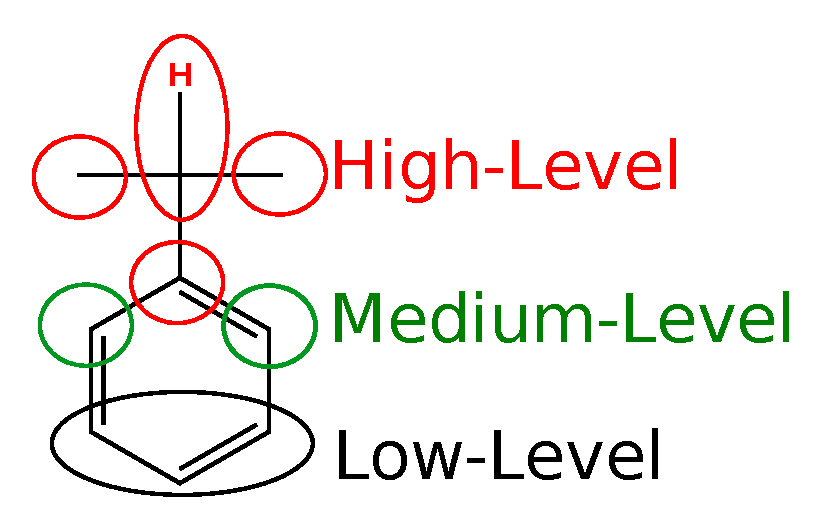
\includegraphics[width=\textwidth]{figures/ldbs.eps}
\caption[Locally-dense basis set partitioning used in the calculation of BDEs.]{Locally-dense basis set partitioning used in the calculation of BDEs. The scheme is referred to as pc-3/3/2/1, where for the shown cumene molecule, the centre of \ch{C-H} cleavage and the immediately adjacent groups are treated with high-level pc-3 basis sets. The next groups are treated with medium level pc-2 basis sets, and all other atoms are treated with low-level pc-1 basis sets.}
\label{fig:ldbs}
\end{scheme}

\noindent \textbf{CBS methods}

The Complete Basis Set (CBS) methods of Petersson and coworkers\cite{Montgomery1999, Montgomery2000, Ochterski1996, Wood2006} are widely used because of the relatively low computational cost (compared to other composite procedures), and well established accuracy.\cite{Somers2015, Simmie2015} CBS-QB3\cite{Montgomery1999, Montgomery2000} utilises DFT-based B3LYP optimisation and scaled frequencies (factor = 0.990) with modified triple-zeta Pople style basis sets. Electronic energies are obtained by extrapolation of medium basis set CCSD(T) and MP4SDQ. Small empirical corrections for are added to achieve more accurate results compared to the parametrisation sets.\cite{Petersson2001} ROCBS-QB3 is a similar procedure to CBS-QB3, except spin-resticted wave functions are used in place of unrestricted wave functions. This is done to eliminate spin contamination, and the use of an restricted open-shell definition has been shown to produce more accurate BDEs.\cite{DiLabio1999} (RO)CBS-QB3 has been implemented for first, second, and third periods of elements.

Atomic pair natural orbital (APNO) expansions are a method used for averaging over multiple Slater determinants. The use of APNOs allows for small basis set extrapolation of higher order correlation energies to converge more rapidly to the complete basis set limit. This approach is used in the CBS-APNO method.\cite{Ochterski1996} Geometries and scaled frequencies (factor = 0.989) are obtained at the QCISD/6-311G(d,p) level of theory. Similar to CBS-QB3, the extrapolation of moderate basis set MP4SDQ and QCISD(T) results gives the electronic energy. An empirical correction is also used in CBS-APNO. Even though CBS-APNO is more accurate, the expansion of APNOs makes CBS-APNO more computationally demanding than CBS-QB3. As a results, it has only been implemented for first and second row periods, and is thus less commonly used in literature.
\\

\noindent \textbf{G$n$ methods}

The Gaussian$-n$ (G$n$) series of methods originate from the Pople group,\cite{Pople1989} where G4 is the fourth generation. G4 utilises moderately large basis sets and extrapolation techniques with CCSD(T) calculations to obtained highly correlated electronic energies. G4(MP2) uses MP2 in place is CCSD(T) and is thus less computationally expensive, but also gives a less complete description of electron correlation. Both methods use the B3LYP/6-31(2df,p) level of theory for optimisation and frequency calculations with a frequency scaling factor of 0.9854. G4 results have been described as generally on par with CBS-QB3 results,\cite{Somers2015, Simmie2015} but calculations are more computationally expensive.

\subsection{Transition state calculations}

Calculations were performed to identify the lowest energy TS complex of several reactions between \cumo~ and organic substrates. In all cases cisoid and transoid conformations were explored. All optimisation calculations were performed at the B3LYP-D3(BJ)/6-31+G$^*$ level of theory, followed by single-point energy calculations at the LC-$\omega$PBE-D3(BJ)/6-311+G$^{**}$ level of theory. The latter DFT-based method was selected to minimise delocalisation error in the TS complex.\cite{OterodelaRoza2014} Transition states were visualised using the Chemcraft program\cite{ccraft} to confirm a single imaginary frequency connecting reactants to products. In some cases, a small secondary imaginary frequency was observed, indicating a TS complex which is not fully optimised. Necessary steps were taken to re-optimise the structures and eliminate the small imaginary frequencies, however, this was not always successful. Nonetheless, I am confident the structures reported herein sufficiently represent the true TS complex geometries and relative energies. Results from stuctures which are not fully optimised are indicated as such appropriately.

\section{Comparison of composite method for the prediction of BDEs}

In order to determine the best method for BEP principle analysis, and to investigate which is the most efficient yet accurate composite method, the BDEs of 49 species have been calculated. This set of species contains a wide variety of chemical functionalities with bond strengths ranging from 75--113 \kcalmol, thus this set may be described as a comprehensive test of these methods for C-H BDEs. Given that W1BD is the most accurate method used, these results have been used for comparison to other composite method. However, BDEs for only 33 out of the 49 species studied were able to be calculated using W1BD due to computational cost restrictions: hard disk capacity was insufficient for large systems. Therefore, literature BDEs from \citet{Luo2002} for all species in the set are also used for comparison. The literature and calculated BDEs are listed in~\ref{tab:bde-calc}.

\begin{landscape}
%\singlespacing
\newcommand{\tabBDE}[2][0.7]{\includegraphics[scale=#1]{figures/#2.eps}}
\setlength\LTleft{-1.5cm}
\begin{longtable}{m{3.5cm} >{\centering}m{3.5cm} | >{\centering}m{0.8cm} >{\centering}m{0.9cm} >{\centering}m{3cm} >{\centering}m{0.9cm} m{0em}}
\caption[Bond dissociation enthalpies of the species used to investigate the accuracy of composite methods.]{Bond dissociation enthalpies of the species used to investigate the accuracy of composite methods. Structures show an explicit C-H bond for that which is cleaved. All values are in \kcalmol. Statistics are listed at the bottom of the table.} \label{tab:bde-calc} \\
Molecule                         & Structure &  Lit.     &   W1BD   &   ROCBS-QB3 &    G4   &\\
\hline
% \endfirsthead
% Molecule                         & Structure &  Lit.     &   W1BD   &   ROCBS-QB3 &    G4   &\\
% \hline
% \endhead
1,3-pentadiene                   & \tabBDE{BDEs/13pentadiene} &  83.0     &   82.9   &     81.7    &   81.6  &\\
1,4-cyclohexadiene               & \tabBDE{BDEs/14cyclohexadiene} &  76.0     &   76.3   &     75.0    &   75.2  &\\
1,4-diazabicyclo[2.2.2]-octane   & \tabBDE{BDEs/DABCO} &  93.4     &          &     98.8    &   96.7  &\\
1,4-pentadiene                   & \tabBDE{BDEs/14pentadiene} &  76.6     &   76.2   &     75.0    &   75.1  &\\
2,2-dimethylbutane               & \tabBDE{BDEs/22dimethylbutane} &  98.0     &   99.3   &     99.3    &   97.5  &\\
2,3-dimethylbutane               & \tabBDE{BDEs/23dimethylbutane} &  95.4     &   97.8   &     97.8    &   96.2  &\\
2-methylbutane                   & \tabBDE{BDEs/2methylbutane} &  95.8     &   97.3   &     97.1    &   95.9  &\\
9,10-dihydroanthracene           & \tabBDE[0.5]{BDEs/dhanthracene} & 76.3     &          &     78.1    &          &\\
Acetaldehyde                     & \tabBDE{BDEs/acetaldehyde} &  94.3     &   95.9   &     95.7    &   94.9  &\\
Acetone                          & \tabBDE{BDEs/acetone} &  96.0     &   96.9   &     96.7    &   95.4  &\\
Acetonitrile                     & \tabBDE{BDEs/acetonitrile} &  97.0     &   96.9   &     96.6    &   96.3  &\\
Adamantane (2$^\circ$)           & \tabBDE{BDEs/adm-sec} &  98.4     &          &    100.4    &   97.8  &\\
Adamantane (3$^\circ$)           & \tabBDE{BDEs/adm-tert} &  96.2     &          &     99.9    &         &\\
Benzaldehyde                     & \tabBDE{BDEs/benzaldehyde} &  88.7     &          &     91.4    &   89.3  &\\
Benzene                          & \tabBDE{BDEs/benzene} & 112.9     &  113.1   &    113.0    &         &\\
Benzyl Alcohol                   & \tabBDE{BDEs/benzylalcohol} &  79.0     &          &     83.2    &   83.4  &\\
Cumene                           & \tabBDE{BDEs/cumene} &  83.2     &          &     86.9    &   86.9  &\\
Cycloheptane                     & \tabBDE{BDEs/cycloheptane} &  94.0     &          &     95.8    &   93.9  &\\
Cyclohexane                      & \tabBDE{BDEs/cyclohexane} &  99.5     &   99.2   &     99.3    &   97.5  &\\
Cyclooctane                      & \tabBDE{BDEs/cyclooctane} &  94.4     &          &     92.4    &   90.2  &\\
Cyclopentane                     & \tabBDE{BDEs/cyclopentane} &  95.6     &   96.3   &     96.3    &   95.6  &\\
Cyclopropane                     & \tabBDE{BDEs/cyclopropane} & 106.3     &  109.0   &    109.2    &  108.2  &\\
Dibenzyl ether                   & \tabBDE[0.4]{BDEs/dibenzylether} &  85.8     &          &     82.7    &         &\\
Diethyl ether                    & \tabBDE{BDEs/diethylether} &  93.0     &   95.3   &     95.5    &   93.8  &\\
Dimethylamine                    & \tabBDE{BDEs/dimethylamine} &  94.2     &   92.6   &     92.8    &   92.0  &\\
Dimethylsulfoxide                & \tabBDE{BDEs/DMSO} &  94.0     &  102.0   &    102.3    &  100.9  &\\
Dioxane                          & \tabBDE{BDEs/dioxane} &  96.5     &   97.3   &     97.6    &   95.7  &\\
Diphenylmethane                  & \tabBDE[0.5]{BDEs/diphenylmethane} &  84.5     &          &     82.8    &         &\\
Ethane                           & \tabBDE{BDEs/ethane} & 100.5     &  101.3   &    101.5    &  100.7  &\\
Ethylbenzene                     & \tabBDE{BDEs/ethylbenzene} &  85.4     &          &     87.6    &   87.6  &\\
Ethylene                         & \tabBDE{BDEs/ethylene} & 110.9     &  110.8   &    110.9    &  109.9  &\\
Fluorene                         & \tabBDE[0.5]{BDEs/fluorene} &  82.0     &          &     81.9    &         &\\
Formaldehyde                     & \tabBDE{BDEs/formaldehyde} &  88.0     &   88.6   &     88.9    &   88.2  &\\
Hexamethyl-phosphoramide         & \tabBDE{BDEs/HMPA} &           &          &     93.9    &         &\\
Indene                           & \tabBDE{BDEs/indene} &  83.0     &          &     80.1    &   79.0  &\\
Methane                          & \tabBDE{BDEs/methane} & 105.0     &  105.0   &    105.2    &  104.5  &\\
Methanol                         & \tabBDE{BDEs/methanol} &  96.1     &   96.4   &     96.8    &   96.0  &\\
Methylamine                      & \tabBDE{BDEs/methylamine} &  93.9     &   93.1   &     93.3    &   92.7  &\\
Morpholine                       & \tabBDE{BDEs/morpholine} &  92.0     &          &     93.3    &   91.8  &\\
N,N-dimethylacetamide            & \tabBDE{BDEs/DMA} &  91.4     &   99.6   &     99.5    &   97.6  &\\
Piperazine                       & \tabBDE{BDEs/piperazine} &  93.0     &   93.4   &     93.5    &   91.9  &\\
Piperidine                       & \tabBDE{BDEs/piperidine} &  89.5     &   92.1   &     92.2    &   90.7  &\\
Propane                          & \tabBDE{BDEs/propane} & 100.9     &  101.6   &    101.8    &  100.7  &\\
Pyrrolidine                      & \tabBDE{BDEs/pyrrolidine} &  89.0     &   90.8   &     90.7    &   89.5  &\\
Tetrahydro-2H-pyran              & \tabBDE{BDEs/oxane} &  96.0     &   96.3   &     96.5    &   94.7  &\\
Tetrahydrofuran                  & \tabBDE{BDEs/THF} &  92.1     &   93.7   &     93.8    &   92.2  &\\
Toluene                          & \tabBDE{BDEs/toluene} &  89.7     &   90.5   &     89.7    &   89.8  &\\
Trichloromethane                 & \tabBDE{BDEs/trichloromethane} &  93.8     &   93.5   &     93.7    &   92.4  &\\
Triethylamine                    & \tabBDE{BDEs/triethylamine} &  90.7     &          &     91.2    &   89.4  &\\
Trifluormethane                  & \tabBDE{BDEs/trifluoromethane} & 106.4     &  107.2   &    107.4    &  105.8  &\\
\hline
\textbf{Statistics}              & & Lit.      &  W1BD    &  ROCBS-QB3 &     G4   &\\
\hline
Number of BDEs               &($N$) &    49     &     33   &      50    &     43   &\\
MAE (Lit.)                       & &           &   0.82   &    1.64    &   1.21   &\\
Max. Error                       & &           &   1.59   &    3.15    &   4.19   &\\
Min. Error                       & &           &  -8.22   &   -8.25    &  -6.86   &\\
MAE (W1BD)                       & &           &          &    0.18    &   0.70   &\\
Max. Error                       & &           &          &    1.26    &   2.05   &\\
Min. Error                       & &           &          &   -0.35    &   0.37   &\\
\end{longtable}
\setlength\LTleft{0pt}
\setlength\LTright{0pt}

\end{landscape}

Mean absolute error (MAE) is used to assess the quality of computational methods, where errors are calculated with respect to benchmark values for a given data set.\cite{Savin2014} The MAE is calculated as

\begin{equation}
  \mathrm{MAE} = \frac{1}{N} \sum | E_{ref} - E_{calc}|
\end{equation}

\noindent where, for a set of $N$ reference values, the MAE is the average of the mean differences of the reference energy ($E_{ref}$) and the calculated value ($E_{calc}$). The MAE with respect to W1BD and literature shall be reported herein as ``MAE$_{\mathrm{W1BD}}$ (MAE$_{\mathrm{Lit.}}$)''. An additional semi-quantitative metric which I used to evaluate the accuracy of composite procedures to reproduce experimental results, is a bar chart which summarises the number of deviations from literature within given error ranges. This bar chart is reported in~\ref{fig:maebarchart}. Also, an alternative method for visualising these data is through the use of one-to-one plots, in which BDEs from two methods are directly compared. An ideal plot should have a slope = 1 and y-intercept = 0.

\begin{figure}[H]
  \centering
  \includegraphics[width=\textwidth]{figures/bde-barchart}
  \caption[Summary of deviations of BDEs from literature for composite quantum chemical methods.]{Summary of deviations of BDEs from literature or composite quantum chemical methods. Errors are units of \kcalmol and are relative to Reference~\protect\citenum{Luo2002}. Numbers out of 49 represent the total number of data points which were computed for the given method.}
  \label{fig:maebarchart}
\end{figure}

Comparing W1BD results to literature, the MAE is 0.82 \kcalmol, where the majority of the data matching to within 1--2 \kcalmol of literature. Thus, W1BD is largely consistent with the literature values. Additionally, the one-to-one plots comparing W1BD to literature in~\ref{fig:1-1-W1BD}, show reasonable agreement with slope of 0.98 and a y-intercept of 2.35. There are, however, two large outliers: dimethyl sulfoxide\footnotemark~ and \emph{N,N}-dimethylacetamide, with experiment underestimating the BDEs by -8.0 and -8.2 \kcalmol, respectively. These large outliers are consistent amongst all composite method, suggesting the literature BDEs for dimethyl sulfoxide and \emph{N,N}-dimethylacetamide are incorrect.

\footnotetext{The experimental BDE for dimethyl sulfoxide was previously identified as accurate by Salamone et al.\protect\cite{Salamone2012}}

\begin{figure}[H]
  \centering
  \includegraphics[width=\textwidth]{figures/lit-w1bd}
  \caption[One-to-one plot of BDEs from literature and as calculated by the W1BD composite method.]{One-to-one plot of BDEs from literature\protect\cite{Luo2002} and as calculated by the W1BD composite method. The red line represents the least squares line of best fit, while black line represents a perfect one-to-one correlation.}
  \label{fig:1-1-W1BD}
\end{figure}

The method which gives the best combined agreement with W1BD and literature is ROCBS-QB3 wiht an MAE = 0.18 (1.64) \kcalmol. It is also apperant from the one-to-one plots in~\ref{fig:1-1-ROCBSQB3}, that ROCBS-QB3 matches well with literature and experiment. In comparison, CBS-QB3 has an MAE = 0.32 (1.88) \kcalmol, while CBS-APNO has an MAE = 0.20 (1.40) \kcalmol. The LDBS approach also performs well with an MAE = 0.22 (1.60) \kcalmol. The G4 method deviates from the W1BD reference by about 0.5 \kcalmol more, however, it appears to give reasonable agreement with experimental results (MAE = 0.70 (1.21) mol). The use of the MP2 variant of G4 gives somewhat questionable results, with an MAE of 0.88 (1.60) \kcalmol, as well as a large outlier of 6.2 kcal/mol that is not present in the other data from composite methods. One-to-one plots of all other methods are presented in Appendix~\ref{ap:bde}.

\begin{figure}[H]
  \hspace*{-1.5cm}
  \begin{minipage}{8cm}
    \centering
    \includegraphics[width=\textwidth]{figures/lit-rocbsqb3}
  \end{minipage}%
  \begin{minipage}{8cm}
    \centering
    \includegraphics[width=\textwidth]{figures/w1bd-rocbsqb3}
  \end{minipage}
  \caption[One-to-one plot comparing calculated BDEs calculated by ROCBS-QB3 to literature and W1BD BDEs.]{One-to-one plot comparing calculated BDEs calcualted by the ROCBS-QB3 to reference literature\protect\cite{Luo2002} and W1BD BDE values, respectively. The red line represents the least squares line of best fit, while black line represents a perfect one-to-one correlation.}
  \label{fig:1-1-ROCBSQB3}
\end{figure}

In summary, ROCBS-QB3 performs best for the calculation of \ch{C-H} BDEs while G4(MP2) performs worst. Given these data, and considering the relative computational cost, the ROCBS-QB3 method is recommended for the calculation of accurate BDEs, particularly for large molecules for which more expensive computational methods are not possible. Importantly, we can now confidently continue investigating the BEP relationships using reliable calculated BDE data from the ROCBS-QB3 method. Furthermore, these results can be extended to even larger systems as the ROCBS-QB3 approach is one of the least computationally expensive composite methods. For example, for calculations on the cyclohexane molecule, which take about 20 minutes using ROCBS-QB3 on SGI Altix compute nodes with 6 processors and 8 GB RAM, while G4 takes about 27 times longer, the LDBS approach takes about 500 times longer, and W1BD takes about 1100 times longer.

\section{Analysis of the Bell-Evans-Polanyi principle}

We turn now to the application of accurate BDEs on the BEP principle. Experimental HAT rate constants have been collected for 32 reactions involving \cumo and organic substrates. The BEP plot of the logarithm of rate constants divided by the number of equivalent H atoms (i.e. normalised) against BDEs is shown in~\ref{fig:bde-bep}.

There clearly exists two distinct regions in~\ref{fig:bde-bep}, inline with our initial hypothesis that there should exist two linear relations: one for benzylic/allylic C-H bonds and another for alkyl C-H bonds. However, the correlation of one of these trends is poor, a result which is inconsistent with our hypothesis. For the series of C-H BDEs which result in a radical which is delocalised, the correlation coefficient is 0.89, suggesting a valid correlation. Therefore, there is predictive power from a BEP relation for C-H bond cleavage which results in a delocalised radical. Furthermore, this result is consistent with the correlation of rate constants with C-H BDEs for model unsaturated fatty acids, described by Pratt et al.\cite{Pratt2003}

\begin{figure}[H]
  \centering
  \includegraphics[width=\textwidth]{figures/bde-bep}
\begin{tabularx}{\textwidth}{| l X l X |}
  \hline
  1 & Acetone & 2 & Acetonitrile \\
  3 & Cyclopentane & 4 & 2,2-dimethylbutane \\
  5 & 2,3-dimethylbutane & 6 & Cyclohexane \\
  7 & Cycloheptane & 8 & Cyclooctane \\
  9 & Adamantane (2$^\circ$) & 10 & Adamantane (3$^\circ$) \\
  11 & Diethyl ether & 12 & Piperazine \\
  13 & Piperidine & 14 & Pyrrolidine \\
  15 & Tetrahydrofuran & 16 & Dioxane \\
  17 & Triethylamine & 18 & 1,4-diazobicyclo[2.2.2]octane \\
  19 & Dimethyl sulfoxide & 20 & Benzaldehyde \\
  21 & Hexamethylphosphoramide & 22 & Morpholine \\
  23 & Diethylamine & 24 & Propylamine \\
  25 & 1,4-cyclohexadiene & 26 & Toluene \\
  27 & Benzyl alcohol & 28 & Ethylbenzene \\
  29 & Cumene & 30 & Diphenylmethane \\
  31 & Dibenzyl ether & 32 & 9,10-dihydroanthracene \\
  \hline
\end{tabularx}
  \caption{Bell-Evans-Polanyi plot of experimental rate constants (normalised for the number of equivalent hydrogen atoms) for HAT between \cumo~ and substrates. Acetone and acetonitrile are note included in fitting as the experimental rate constants are approximate. Needs revision to move labels around.}
\label{fig:bde-bep}
\end{figure}

\jnote{fix}
In contrast, the alkyl C-H BDEs shows very weak correlation with HAT rate constants, with a correlation coefficient of 0.63. However, with the exception of two larger outlier, cyclooctane and the secondary hydrogen position of adamantane, the majority of the data fall within half an order of magnitude of rate a rate constant which is consistent with the line of best fit. The two large outliers are approximately twice as far from the trendline. While this result may not seem positive, there is actually some predictive power in the BEP relation established for alkyl C-H bonds. This is because in the calculations of rate constants, an error of only 1.2 \kcalmol can result in a order of magnitude difference in rate constant. Errors of this magnitude are not uncommon for DFT-based mechanistic studies. For example, barrier heights for a set\cite{Zhao2005, Zhao2009} of 76 hydrogen transfer, heavy atom transfer, nucleophilic substitution, unimolecular, and association reactions calculated with at the B3LYP-D3(BJ)/Def2-QZVP level of theory give a mean absolute error of 5.20 \kcalmol, with errors exceeding 11 \kcalmol.\cite{Goerigk2011}

In sum, these results suggest that the BEP principle is overly simple to directly correlate the large groups of allylic/benzylic and alkyl C-H bonds with HAT rate constant. Nonetheless, BEP relations offer predictive capabilities for rate constants to within an order of magnitude. Importantly, this result indicates that there are additional factors which contribute to the HAT rate constants studied herein.

\section{Transition state analysis}

In order to determine what effects appear to be most important, I have calculated TS structures for 20 of the reactions at the LC-$\omega$PBE-D3(BJ)/6-311+G(2d,2p)//B3LYP-D3(BJ)/6-31+G$^*$ level of theory. Comparing the calculated rate constants both with and without tunnelling corrections, there is a large degree of variability in the agreement with experiment. \ref{fig:kH-theory} demonstrates that the calculated rate constants deviate rather significantly from the experimental rate constants, both with and without the inclusion of a tunnelling correction. This result is perhaps unsurprising given the neglect of solvent effects, and the fairly low level of theory used for optimisation. Note however, that the goal of these calculations was not to reproduce experimental rate constants, but to obtain TS complex structures to analyse the structural differences that may lead to the deviations from the BEP principle.

\begin{figure}[htb]
\hspace*{-1.5cm}
\begin{minipage}{8cm}
  \centering
  \includegraphics[width=\textwidth]{figures/kH-theorya}
\end{minipage}%
\begin{minipage}{8cm}
  \centering
  \includegraphics[width=\textwidth]{figures/kH-theoryb}
\end{minipage}
\caption[One-to-one plots of theoretically determined logarithm of rate constant or HAT reactions between \cumo~ and organic substrates against experimental values.]{One-to-one plots of theoretically determined logarithm of rate constant for HAT reactions between \cumo~ and organic substrates against experimental values. The plot on the left does not include a tunnelling correction while the plot on the right includes the Eckart potential tunnelling correction.}
\label{fig:kH-theory}
\end{figure}

The first factor which may lead to deviations from the BEP is the possibility for different HAT reaction mechanisms, i.e. direct HAT or PCET. Consider first the reaction of toluene with \cumo. As this reaction is similar to the self-exchange reaction of the benzyl-toluene couple as described by DiLabio and Johnson,\cite{DiLabio2007} one might expect the reaction to proceed via PCET. The lowest energy TS complex has a partially $\pi$-stacked conformation with the rings oriented about 40$^\circ$ relative to one another. Surprisingly, examination of the SOMO and HOMO reveals no $\pi$-$\pi$ partial bonding interaction, as can be seen in~\ref{fig:cumo-toluene}. The electron density of the SOMO is largely localised on the toluene portion of the complex. This is likely due to the additional non-conjugated carbon centre of \cumo, which prevent an additional electron channel for PCET to occur. Therefore, this reaction takes place through direct HAT. This behaviour is specific to the \cumo radical, thus all the reactions likely also take place through a direct HAT mechanism, and this should not factor into the deviations in the observed BEP principle relationships.

\begin{figure}[htb]
  \includegraphics[width=\textwidth]{figures/cumo-toluene}
  \caption{Insert better images of \cumo-toluene TS complex with A) SOMO and B) HOMO.}
  \label{fig:cumo-toluene}
\end{figure}

There are several other possible deviations which may arise from differences in intermolecular interactions due to structural differences in the substrates. For example, cyclooctane may deviate from the trend observed due to the many possible conformations of the ring which are comparable in energy.\cite{Dorofeeva1985} Alternatively, the position of the TS complex along the reaction coordinate may differ between the various reactions. This would break the assumption of the BEP principle, and may result in deviation from the expected trend.

\jnote{I am having a hard time finding further explanations from the data I have. Any input here is greatly appreciated.}

\section{Summary}

Firstly, a number of composite quantum mechanical methods were tested for the accurate prediction of C-H BDEs. The ROCBS-QB3 method was determined to be the most efficient accurate method for this purpose. Additionally, the widespread applicability of the BEP principle was investigated through utilisation of these accurate C-H BDEs and experimental HAT rate constants for reaction of \cumo with organic substrates.

As was hypothesised, two relationships exist for the BEP principle when investigating a wide range of HAT reactions from C-H bonds. C-H bonds which result in a radical which can be delocalised into neighbour $\pi$ systems (benzylic/allylic) correlate well with experimental rate constants. The remaining alkyl C-H bonds, correlate weakly with experimental rate constants and offer only order of magnitude predictions of rate constants. Altogether, these results suggest that the BEP principle must be carefully applied if accurate rate constants are the desired target, however, they also suggest that as the BEP principle holds as a reasonably general principle.


% !TEX root = diss.tex

\chapter{Do non-redox active metal cations have the potentials to behave as chemo-protective agents? The Effects on Metal Cations on HAT Reaction Barrier Heights}
\label{ch:hat}

\section{Introduction}

Metal cations are ubiquitous in biological systems and play an important role in biological function. As such, there is a great deal of interest in studying metals in biological systems. Proteins in particular are often associated with metals, and in the worldwide Protein Data Bank,\cite{Harding2010, Berman2007} over one-third of crystal structures contain metals. Redox active metals, such as copper and iron, act as co-factors in metalloenzymes for important catalytic processes.\cite{Atkins2010}

Non-redox active metal cations are equally as important in biological function as redox active metals, where they are essential to protein structure and function, along with cellular and neuronal signaling.\cite{Karp1999} Sodium and calcium ions are most abundant extracellurly, while potassium and magnesium are dominant inside of cells. While specific ionic concentrations vary dramatically dependening on physiological conditions, estimates for equilibrium concentrations in both mammalian heart cells\cite{Ingwall2006} and blood plasma\cite{daSilva2001} are listed in~\ref{tab:metalconc}. As sodium and magnesium are most abundant alkali and alkaline earth metals found in biologically relevant systems, they are of prime interest for investigation.

\begin{table}[!htbp]
  \caption{Ionic concentrations inside a mammalian heart cell and in the blood plasma. Concentrations are in units of mM. Values are rounded to one significant figure. Data are from Ref. \protect\citenum{Ingwall2006} and \protect\citenum{daSilva2001}.}
  \label{tab:metalconc}
\begin{tabular}{l c c}
  Ion Conc. & Mammalian Cells & Blood Plasma \\
  \hline
  \ch{Na^+} & 10 & 100--200 \\
  \ch{Mg^{2+}} & 10 & 1 \\
  \ch{K^+} & 100 & 4 \\
  \ch{Ca^{2+}} & 0.1 & 2
\end{tabular}
\end{table}

Extensive crystallographic surveys indicate that metals bind predominantly to oxygen centres in proteins.\cite{Harding1999, Harding2004, Hsin2008} Divalent metals are most often found bound directly to proteins. Calcium binds anywhere from 4 to 6 binding sites in protein crystal structures, while magnesium binds only 1 or 2. Monovalent metals, on the other hand, are often heavily solvated and so they appear in solvent cavities of proteins, although sodium or potassium are sometimes found bound directly to carbonyl or carboxylate oxygen centres.\cite{Harding2010}

A great deal of research has focussed on \ch{Ca^{2+}} in the context of reactive oxygen-centred radical production.\cite{Goerlach2015} Specifically, \ch{Ca^{2+}} ions are important in the mitochondria, where, depending on physiological conditions and concentrations, they can act as inhibitor or promoters of free-radical production in the electron transport chain.\cite{AdamVizi2010} In explanation is that \ch{Ca^{2+}} induce conformational changes of the proteins involved in the electron transport chain which are responsible for radical generation.\cite{Brookes2004} Mitochondrial free-radicals, when present in moderate amounts, can act as cell signalling molecules to activate pro-growth responses.\cite{Sullivan2014} However, ``dysfunctional'' mitochondria can produce excess radicals leading to oxidative damage which has been linked to degenerative diseases.

Given the significant importance alkali and alkaline earth metals play in biological systems, their impact on protein oxidation must be considered. However, until recently, kinetic studies of protein oxidation have not investigated the mechanistic role of non-redox active metals. In a series of three papers,\cite{Salamone2013a, Salamone2015metals, Salamone2016} Bietti and colleagues have shown that alkali and alkaline earth metals have an inhibitory effect on HAT reactions involving \cumo\ and organic substrates. Some of the experimental rate constants from these papers are summarized in~\ref{tab:hat-metals}. All rate constants were obtained by time-resolved LFP in nitrogen or argon-saturated acetonitrile (MeCN) at 298 K, as was previously described in Section~\ref{sec:hat-methods}. All of the experimental results have been rationalized on the basis of Lewis acid metals cations interactions with Lewis basic substrates.

\bgroup
\def\arraystretch{1.2}%  1 is the default, change whatever you need
\begin{table}
  \caption{Table summary of experimental data - Needs completion}
  \label{tab:hat-metals}
  \hspace*{-1.2cm}
  \begin{tabular}{l l c c}
    Substrate & Conditions & $k_H$ (\Ms) & $k_H$(MeCN)/$k_H$(M$^{n+}$) \\
    \hline
    1,4-cyclohexadiene &    & 6.7\E{7} & \\
    (CHD)  & \ch{LiClO4} 1.0 M & 7.5\E{7} & 0.89 \\
     & \ch{Mg(ClO4)2} 1.0 M & 7.0\E{7} & 0.96 \\
    tetrahydrofuran &   & 5.7\E{6} & \\
    (THF) & \ch{LiClO4} 1.0 M & 2.9\E{6} & 1.7 \\
     & \ch{LiOTf} 1.0 M & 2.8\E{6} & 2.0 \\
     & \ch{Mg(ClO4)2} 1.0 M & 1.8\E{6} & 3.2 \\
    triethylamine &  & 2.0\E{8} & \\
    (TEA) & \ch{LiClO4} 1.0 M & 9.4\E{7} & 2.1 \\
     & \ch{Mg(ClO4)2} 0.005 M & $<$1\E{6} & $>$200 \\
    $N,N$-dimethylformamide & & 1.2\E{6} & \\
    (DMF) & \ch{LiClO4} 0.5 M & $k_{H1}$ = 8.9\E{5} & 1.3 \\
      & & $k_{H2}$ = 1.5\E{6} & 0.80 \\
      & \ch{NaClO4} 0.2 M & $k_{H1}$ = 9.6\E{5} & 1.3 \\
      & & $k_{H2}$ = 1.4\E{6} & 0.86 \\
      & \ch{Mg(ClO4)2} 0.2 M & $k_{H1}$ = 5.8\E{5} & 2.1 \\
      & & $k_{H2}$ = 1.1\E{6} & 1.1 \\
      & \ch{Ca(ClO4)2} 0.2 M & $k_{H1}$ = 1.0\E{6} & 0.83 \\
    $N,N$-dimethylacetamide &  & 1.2\E{6} & \\
    (DMF) & \ch{LiClO4} 0.2 M & $k_{H1}$ = 8.5\E{5} & 1.4 \\
      & & $k_{H2}$ = 1.5\E{6} & 0.8 \\
      & \ch{NaClO4} 0.2 M & $k_{H1}$ = 1.1\E{6} & 1.1 \\
      & & $k_{H2}$ = 1.3\E{6} & 0.92 \\
      & \ch{Mg(ClO4)2} 0.2 M & $k_{H1}$ = 4.7\E{5} & 2.6 \\
      & & $k_{H2}$ = 2.4\E{5} & 5.0 \\
      & & $k_{H3}$ = 1.1\E{6} & 1.1 \\
      & \ch{Ca(ClO4)2} 0.2 M & $k_{H1}$ = 1.2\E{6} & 1.0
  \end{tabular}
\end{table}
\egroup

Firstly, for hydrocarbons, cyclic ethers, and tertiary amines, \cumo\ hydrogen abstraction rate constants in the presence of excess concentrations of lithium and magnesium salts were measured.\cite{Salamone2013a} In the presence of \ch{LiClO4} and \ch{Mg(ClO4)2}, the rate of abstraction by \cumo\ from 1,4-cyclohexadiene (CHD) increases very slightly. Since CHD has no Lewis basic centres, the increase in HAT rate constant was explained on the basis of metal cation interactions with \cumo, very slightly increasing the hydrogen abstraction ability by withdrawing electron density from the aromatic ring. Metal cations were also shown to increase the unimolecular decay of \cumo\ by $\beta$-scission (See Section~\ref{sec:hat-methods}). The largest kinetic effect was observed with \ch{LiClO4} with $k_\beta$ = 1.8\E{6} $s^{-1}$, which is a
roughly 3-fold increase as compared to the rate in MeCN at 298 K ($k_\beta$\cite{Avila1995} = 6.3\E{5} $s^{-1}$). This effect is significantly less than the observed kinetic solvent effect on \cumo\ $\beta$-scission measured in \ch{H2O} or 2,2,2-trifluoroethanol ($k_\beta$ = 1.0\E{7} and 6.1\E{6} $s^{-1}$, respectively).\cite{Bietti2005, Neta1984} Therefore, the kinetic effects of these alkali and alkaline metal salts interacting via Lewis acid-base interactions with the oxygen-centre of \cumo\ are less than the effects of hydrogen-bonding by solvents.

Next, the HAT rate constants for abstraction from tetrahydrofuran (THF) decrease in the presence of non-redox active metal salts. Both \ch{LiClO4} and \ch{LiOTf} decrease $k_H$ by a factor of about 2, indicating the nature of the counter-anion plays a negligible role in the Lewis acid-base interactions between metal cations and substrates. The addition of \ch{Mg(ClO4)2} has a greater effect on HAT reactivity, decreasing $k_H$ by a factor of 3. Magnesium ions are a stronger Lewis acid than lithium,\cite{Fukuzumi2002} supporting the notion of Lewis acid-base interactions between the oxygen lone-pair and the metal cations. The decrease in $k_H$ has been partially attributed to the reduction in hyperconjugative overlap between the oxygen lone-pair and the neighbouring \ch{C-H} $\sigma^*$ anti-bonding orbital (See~\ref{fig:THF}), as a consequence of the metal cation withdrawing electron density from the oxygen lone-pair.

A 2-fold decrease in $k_H$ for the tertiary amine, triethylamine (TEA), is observed upon the addition of \ch{LiClO4}, for which an analogous orbital interaction explanation is also appropriate. Interestingly, the addition of 1.0 M \ch{Mg(ClO4)2} was reported to immediately form a precipitate to form. This precipitate was identified as the formation of a strong TEA-\ch{Mg^{2+}} Lewis acid-base adduct. This observation is once again consistent with the stronger Lewis acidity of \ch{Mg^{2+}} as compared to \ch{Li^+}, and also the significantly greater Lewis basicity of TEA vs THF.\cite{Salamone2013a, Reichardt2010} It was also pointed out that MeCN will competitively bind with metal cations, however it is a weaker Lewis base than both THF and TEA. Measurements of $k_H$ for HAT between \cumo\ and TEA in the presence of 0.005 M \ch{Mg(ClO4)2} were successful only up until [TEA] = 9.6 mM, at which point a precipitate began to form. Nonetheless, an upper limit to the hydrogen abstraction rate constant was estimated as $k_H <$ 1\E{6} \Ms, or at least a 200 fold decrease relative to no metal salt. Very similar results for bulkier tertiary amines were also obtained. Thus, the presence of strong Lewis acids in the presence of Lewis basic sites on hydrogen atom donors can deactivate \ch{C-H} bonds.

Next, we turn to the more relevant models for the work of this thesis, the tertiary amides $N,N$-dimethylformamide (DMF) and $N,N$-dimethylacetamide (DMA). As with THF, normal hyperconjugative overlap between the conjugated amide $\pi$-system and the adjacent \ch{C-H} $\sigma^*$ anti-bonding orbitals weakens the C-H bonds. Therefore, metal binding to the amide oxygen-centre should result in a decrease in this orbital interaction, strengthen the C-H bonds, and decrease HAT reactivity. In their study, \citet{Salamone2015metals} measured \cumo\ abstraction rate constants from DMF and DMA in the presence of stoichiometric equivalents of \ch{LiClO4}, \ch{LiOTf}, \ch{NaClO4}, \ch{Mg(ClO4)2}, and \ch{Ca(ClO4)2} (in contrast to the excess used in Reference~\citenum{Salamone2013a}). Figure~\ref{fig:k-metals-mg}a,b shows the plots of $k_{obs}$ against [substrate] for the reactions of \cumo with DMF and DMA in MeCN containing 0.2 M \ch{Mg(ClO4)2}, respectively. For both DMF and DMA, there are three distinct regions in the plots: weak C-H bond activation for [amide]/[\ch{Mg^{2+}}]$\leq 2$, followed by strong C-H bond deactivation for 2$<$[amide]/[\ch{Mg^{2+}}]$\leq$4, and no deactivation for [amide]/[\ch{Mg^{2+}}]$<$4.

\begin{figure}[!htbp]
  \includegraphics[width=\textwidth]{figures/kH-dma-dmf-mgclo42.png}
  \caption[Plot of observed rate constant against concentration of DMF and DMA for reaction with \cumo\ at 298 K in the presence of 0.2 M \ch{Mg(ClO4)2}.]
  {\textbf{a)} Plot of observed rate constant against concentration of DMF for reaction with \cumo\ at 298 K in the presence of 0.2 M \ch{Mg(ClO4)2}. 0--0.4 M [DMF] range (black circles), $k_{H1}$ = 5.8\E{5} \Ms; 0.8--2.2 M [DMF] range (white circles), $k_{H2}$ = 1.3\E{6} \Ms.
  \textbf{b)} Plot of observed rate constant against concentration of DMA for reaction with \cumo\ at 298 K in the presence of 0.2 M \ch{Mg(ClO4)2}. 0--0.4 M [DMA] range (black circles), $k_{H1}$ = 4.7\E{5} \Ms; 0.4--0.8 M [DMA] range (grey circles), $k_{H2}$ = 2.4\E{5} \Ms; 0.8--2.2 M [DMA] range (white circles), $k_{H3}$ = 1.1\E{6} \Ms. Reprinted with permission from Reference~\protect\citenum{Salamone2015metals}. Copyright 2015 American Chemical Society.}
  \label{fig:k-metals-mg}
\end{figure}

The addition of both \ch{LiClO4} and \ch{LiOTf} decrease to a similar extent the rate constants for abstraction from DMF and DMA by \cumo. However, in contrast to \ch{Mg(ClO4)2}, the lithium salts strongly deactivate \ch{C-H} bonds for 2 equivalents, followed by weak deactivation for another 2 equivalents, and no deactivation for [amide]/[\ch{Li^{+}}]$<$4. Salamone et al. were not able to give a clear cut explanation, but suggest that the different patterns are a result of differences in charge density, which is greater for \ch{Mg^{2+}} than \ch{Li^+}, as well as different coordination geometries of the two ions. A coordination number of 4 is most common for \ch{Li^+}, while an octahedral geometry with the coordination of 6 ligands is almost always observed for \ch{Mg^{2+}}.\cite{Babu2013, Dudev2014} As a result, interactions of the ions with solvent and counter-anions are suggested to be more important for \ch{Mg^{2+}} than \ch{Li^+}.

\ch{NaClO4} and \ch{Ca(ClO4)2} influence HAT between \cumo\ and DMA to different extents than both \ch{LiClO4} and \ch{Mg(ClO4)2}. Figure~\ref{fig:k-metals-naca}a,b shows the plots of $k_{obs}$ against [substrate] for the reactions of \cumo with DMA in MeCN containing 0.2 M \ch{NaClO4} and \ch{Mg(ClO4)2}, respectively. For \ch{NaClO4}, an almost negligible deactivation of \ch{C-H} bonds is observed for up to 4 equivalents of DMA. This was explained on the basis of the weaker Lewis acidity of \ch{Na^+} as compared to \ch{Li^+}. With regards to \ch{Ca(ClO4)2}, binding to DMA fully deactivates \ch{C-H} bond abstraction up to 4 equivalents of DMA. The first region of~\ref{fig:k-metals-naca}b ([DMA] = 0--0.2 M, black circles) represents the decrease in $k_\beta$ of \cumo as \ch{Ca^{2+}} preferentially binds to DMA over \cumo. Interstingly, for both DMF and DMA, the same experiments in dimethyl sulfoxide (DMSO) solvent show no inhibition of HAT reactivity by metal cations. This was rationalized on the basis of the stronger Lewis basicity of DMSO as compared to both MeCN and the amides, thus the metals preferentially bind solvent rather than amide substrate.

\begin{figure}[!htbp]
  \includegraphics[width=\textwidth]{figures/exptdma-na-ca.png}
  \caption[Plot of observed rate constant against concentration of DMA for reaction with \cumo\ at 298 K in the presence of 0.2 M \ch{NaClO4} and \ch{Mg(ClO4)2}.]
  {\textbf{a)} Plot of observed rate constant against concentration of DMA for reaction with \cumo\ at 298 K in the presence of 0.2 M \ch{NaClO4}. 0--0.8 M [DMA] range (black circles), $k_{H1}$ = 9.6\E{5} \Ms; 0.8--1.4 M [DMA] range (white circles), $k_{H2}$ = 1.4\E{6} \Ms.
  \textbf{b)} Plot of observed rate constant against concentration of DMA for reaction with \cumo\ at 298 K in the presence of 0.2 M \ch{Ca(ClO4)2}. 0.8--1.7 M [DMA] range (white circles), $k_{H1}$ = 1.2\E{6} \Ms. Adapted with permission from Reference~\protect\citenum{Salamone2015metals}. Copyright 2015 American Chemical Society.}
  \label{fig:k-metals-naca}
\end{figure}

Finally, \citet{Salamone2016} examined the effects of substrate structure on HAT reaction between \cumo and tertiary alkanamides in the presence of alkali and alkaline earth metal ions. For $N,N$-dialkylacetamides, the steric bulk of the $N$-alkyl groups was previously characterized.\cite{Salamone2014} Steric repulsion between \cumo\ and the $N$-alkyl groups can decreases the HAT rate constant, as evident by the 3-fold decrease in $k_H$ in going from DMA to $N,N$-diisobutylacetamide (DIA; 1.2\E{6} and 3.1\E{5} \Ms, respectively). For reactions of \cumo\ with DIA addition of 0.2 M \ch{LiClO4} or \ch{Ca(ClO4)2} to results in the same trends in \ch{C-H} bond deactivation observed for DMA. This indicates that the influence of metal cation-substrate binding is not significantly influences by the steric bulk of $N$-alkyl groups.  The same is true for the addition of 0.2 M \ch{Mg(ClO4)2} to abstraction from DIA by \cumo, as shown in~\ref{fig:k-dia-mg}. Once again, an slight decrease in reactivity is observed for the first 2 equivalents of DIA, followed by strong C-H bond deactivation for an additional two equivalents, and no deactivation beyond that. No additional insight was provided by Salamone et al. as to the reason for this reactivity. The plausible explanation provided was once again that \ch{Mg^{2+}} has a high charge density. These results show that Lewis acid-base interactions between alkali or alkaline earth metal cations can greatly depress hydrogen abstraction by alkyoxyl radicals.

\begin{figure}[!htbp]
  \includegraphics[width=0.6\textwidth]{figures/exptdia-mg.png}
  \caption[Plot of observed rate constant against concentration of DIA for reaction with \cumo\ at 298 K in the presence of 0.2 M \ch{Mg(ClO4)2}.]
  {Plot of observed rate constant against concentration of DIA for reaction with \cumo\ at 298 K in the presence of 0.2 M \ch{Mg(ClO4)2}. 0--0.4 M [DIA] range, $k_{H1}$ = 3.6\E{5} \Ms; 0.8--1.4 M [DIA] range, $k_{H2}$ = 2.9\E{5} \Ms.
  Reprinted from Tetrahedron, 72, Salamone et al., Hydrogen atom transfer from tertiary alkanamides to the cumyloxyl radical. The role of substrate structure on alkali and alkaline earth metal ion induced \ch{C–H} bond deactivation, 7757--7763, 2016, with permission from Elsevier.}
  \label{fig:k-dia-mg}
\end{figure}

With these results in mind, I am interested in the possibility that alkali and alkaline earth metal cations found in biological system can protect \ch{C-H} bonds in proteins from HAT to reactive oxygen-centred radicals. However, the experimental results do not answer some of the key physico-chemical determinants which may make this possible. Specifically, I have composed several important research questions which remain unclear from the experimental results.

The first question which I have is one of methodology: Can DFT-based methods can accurately treat alkali/alkaline metal cation binding to organic substrates or radicals? There exists limited ab initio data describing these interactions.\cite{ Siu2001, Corral2003, Suarez2011, Baldauf2013} Therefore, I have conducted a benchmark quality study involving \ch{Li^+}, \ch{Na^+}, \ch{Mg^{2+}}, \ch{K^+}, and \ch{Ca^{2+}}. to the best of my knowledge, this represents the first systematic benchmark study of these metal cations with both organic substrates, and radicals.

Secondly, the nature of the binding of metal ions to substrates is still poorly described, especially given the odd stoichiometric effects observed for \ch{Mg(ClO4)2} with alkanamides. Specifically, I wish to address the range of these interactions, and how much the metals do effect the C-H being broken. Throughout this investigation I have utilized both \ch{Na^+} and \ch{Mg^{2+}} in my calculations. These metal ions were chosen to capture the large differences in Lewis acidity and ion size associated with these third-period ions, and because they are two of the most biologically relevant metal ions.

Thirdly, I address the effect that metal ions have on the HAT barrier heights.
Experiments demonstrate that under certain conditions the presence of metal ions can decrease HAT reactivity. If metal ions do effectively increase C-H bond strengths, this will certainly be a contributing factor to the free energy barrier. There will likely be additional factors such as polarization in the TS complex, or other effects of possible charge transfer from the substrate to metal ions. To investigate this, I have primarily studied HAT reactions involving DMA and oxygen-centred radicals. I was also interested in structural differences of the oxygen-centred radical, thus I have utilized the \bno and \cumo, which differ significantly in their ability to form strong pre-reaction complexes with hydrogen bond accepting substrates. Note that in this portion of the study, I was met with abundant technical difficulties related to optimizing TS structures including metal cations, and thus the scope of my results and discussion have been reduced.



I have also performed calculations with the bulkier DIA substrate to see if steric bulk does have an influence on the ability of a metal cation to effect HAT reactions.  These results

Finally, I wanted to address the effect of strong Lewis basicity in the hydrogen donating substrate. HAT reactions involving alkoxyl radicals and strong Lewis bases have been previously studied.%\cite{}



\section{Computational methods and details}

All quantum mechanical calculations were performed using either the Gaussian 09 software package,\cite{Frisch2009} or the TURBOMOLE software package.\cite{turbomole} Calculations for the benchmark quality data of metal binding to substrates were first optimized at the LC-$\omega$PBE-D3(BJ)/6-31+G(2d,2p) level of theory,\cite{Vydrov2006, Vydrov2006a, Grimme2010, Johnson2006} and later re-optimized with larger 6-311+G(3df,3pd) basis sets. Single-point energy calculations were then carried out using the coupled cluster methodology with single, double and perturbative triples with full core correlation, CCSD(T,Full), and various basis sets, as will be described in Section~\ref{sec:benchmark}. Final benchmark quality binding energies have been calculated using the F12$^*$ explicitly correlated method with Def2-QZVPPD primary basis sets and Def2-QZVPP auxiliary basis sets required for the resolution-of-the-identity (RI) approximation as implemented in TURBOMOLE. The RI approximation is used to reduce the computational cost associated with calculating MO integrals.\bibnote{For a detail description or the RI approximation and explicit correlation, see Ref.~\protect\citenum{OterodelaRoza2017}, Chapter 4.} At total of 31 different DFT-based methods with nearly complete 6-311+G(3df,3pd) and moderate 6-31+G(2d,2p) basis sets were tested both by single-point energy calculations on the benchmark structures. Geometry optimization calculations starting from the benchmark structures were also performed for three of the best performing DFT-based method, in order to verify their ability to capture the minimum energy bound structures.

To test the effects of metal cations on HAT barrier heights, calculations were first performed for the reactions not involving metal cations. Geometry optimizations were performed at the M05-2X\cite{Zhao2006}/6-31+G$^{**}$ level of theory. Transition state (TS) structures were obtained by first freezing the abstraction donor-hydrogen-acceptor bond lengths with multiple initial orientations. The frozen bonds were then relaxed to obtain the final TS structures, which were then used to identify the appropriate pre- and post-reaction complexes. All structures were subjected to harmonic vibrational frequency calculations, which were visualized using the Chemcraft program\cite{ccraft} to verify minima (or saddle-points with a single imaginary frequency connecting reactants to products for TS structures). Single-point energy calculations were performed at the M05-2X/6-311+G(2d,2p) level of theory. The effects of MeCN solvent were estimated by inclusion of the SMD\cite{Marenich2009} continuum solvent model in single-point energy calculations.

The inclusion of metal cations into the TS structures proved to be technically challenging. It was my expectation that I could simply include metal cations and necessary counter-anions into the minimum energy complex structures and re-optimize, however this was not the case. TS structures were once again obtained by constrained optimization with the inclusion of the metal cation and counter-anion and freezing the abstraction donor-hydrogen-acceptor bond lengths, providing a guess TS structure. However, in most cases the force constants (which are necessary for a TS optimization calculation) from the the guess TS structure were not representative of the true TS structure, thus force constants were recalculated for every step along the optimization, using the ``CalcAll'' keyword in Gaussian. Even using this method, many TS structures including metal cations failed to converge. The final TS structures were once again used to identify the appropriate pre- and post-reaction complexes.

Natural bond order (NBO) and natural population analysis (NPA) were utilized in order to investigate the electronic structures involved in the HAT reactions and the effects of metal cation binding.\cite{Reed1983, Reed1985, Glendening2012} Version 3.1 of the NBO software package,\cite{NBO3} as implemented in the Gaussian 09 package was used in all cases.\cite{Frisch2009}

\section{Benchmarking DFT based methods for the binding of alkali and alkaline earth metals to organic substrates and oxygen centred radicals}
\sectionmark{Benchmarking DFT based methods}
\label{sec:benchmark}

In order to confidently perform quantum mechanical mechanistic studies, the method of choice must be confidently calibrated. While DFT-based methods have been widely applied to these studied, few studies have previously investigated alkali and alkaline earth-metal cation binding to organic substrates.\cite{Corral2003, Suarez2011, Siu2001, Baldauf2013} Most importantly, benchmark quality data for a wide variety of metals binding to biologically relevant substrates and oxygen-centred radicals does not exist to calibrate DFT-based methods. Therefore, I proposed a benchmark study which incorporated all the biologically relevant alkali and alkaline earth-metal cations, models for dipeptides including amino acid side chains, oxygen-centred radicals, and solvents which are utilized in the experimental mechanistic studies involved in probing these systems. Unfortunately, due to computational restrictions (\emph{vide infra}), benchmark quality calculations on the originally proposed benchmark set were not possible. Full details of the originally proposed benchmark set are in Appendix~\ref{ap:hat},~\ref{fig:ap-set1}

Benchmark quality binding energies are generally calculated using the ``gold standard'' approach, CCSD(T)/CBS, where correlation consistent basis sets\cite{Marshall2011, Rezac2013} (cc-pV\emph{X}Z, \emph{X}=T,Q,5) developed by Dunning an\cite{Vydrov2006, Vydrov2006a}d co-workers are used for complete basis set extrapolation. These basis sets have limited availability for the metals of interest. Specifically, basis sets for K are not available, and only non-augmented basis sets for Li, Na, Mg, and Ca. It is necessary to include core-correlation of at least the first core shell in alkali and alkaline earth metals, thus it would be appropriate to use core valence basis sets such as cc-pCV$X$Z.\cite{Peterson2002} However, these basis sets are even more limited. Therefore, I originally chose the augmented version of the polarization consistent basis sets of Jensen and co-workers\cite{Jensen2001, Jensen2002, Jensen2002a, Jensen2003}  (aug-pc-\emph{N}, \emph{N}=2,3,4), which have been shown to converge to the CBS limit systematically\cite{Kupka2007} and are available for all the elements of interest.

While performing CCSD(T)/CBS calculations, I noticed that the metal cations (and neutral metal atoms), did not converge smoothly to the complete basis set limit. As a consequence, complete basis set extrapolation is not feasible. In light of this problem, I decided to re-evaluate the size scope of the benchmark set being used. In order to facilitate future DFT-based work and probe the issue of basis set convergence of alkali and alkaline earth metals, a benchmark set of small substrates was proposed. This new set is shown in \ref{fig:set2}. The new, small benchmark set was selected to include important functional groups and radicals found biological systems, and one of the most common solvents used in physical organic experiments, acetonitrile.

\begin{scheme}[!htbp]
  \centering
    \includegraphics[width=\textwidth]{figures/set2.eps}
    \caption{Revised benchmark set of small substrates and cations. Note this set consists of all combinations of substrates and metal cations, i.e., there are 35 complexes in the set.}
  \label{fig:set2}
\end{scheme}

\subsection{Metal cation basis set convergence}

\begin{figure}[!htbp]
  \centering
    \includegraphics[width=\textwidth]{figures/pes_metals}
    \caption[Basis set convergence for alkali and alkaline earth-metal cations.]{Basis set convergence of CCSD(T,Full)/aug-pc-$N$ ($N$=1,2,3,4) for alkali and alkaline earth-metal cations. The relative energy of each basis set relative to the aug-pc-1 for each metal. The cardinal number of the aug-pc-$N$ basis sets is $X=N+1$.}
  \label{fig:pes_metals}
\end{figure}

In order to perform complete basis set (CBS) extrapolation, the total energy of a molecule/atom should converge smoothly to the CBS limit.\cite{Truhlar1998} However,~\ref{fig:pes_metals} shows the poor basis set convergence of CCSD(T,Full)/aug-pc$N$ ($N$=1,2,3,4) calculations for alkali and alkaline earth-metals. The energy of each ion relative to the smallest basis set is shown. For \ch{Li^+} the value appears to converge reasonably, however this is expected as there are only 2 electrons in this ion. For all of \ch{Na^+}, \ch{Mg^{2+}}, \ch{K^+}, and \ch{Ca^{2+}}, there appears to be no convergence to the CBS limit as each line continues down linearly. This is problematic as it means that CBS extrapolation would result in a significant degree of uncertainty in the estimated CBS limit total energy.

The poor convergence was thought to be a result of poorly suited basis sets to full core-correlation. However, the same CCSD(T,Full) calculations using the core-correlation (cc-pCV$N$Z) basis sets as show unsatisfactory convergence for \ch{Na^+} and \ch{Mg^{2+}} (See Appendix~\ref{ap:hat}, ~\ref{fig:ap_pes_metals}). Therefore, I was tasked with finding a method which would give results which best approximate alkali and alkaline metal binding at the complete basis set limit. I decided to use an explicitly correlated CCSD(T) treatment known as ``F12$^*$'' to more rapidly approach the CBS limit.\cite{Tenno2012} I tested both the core-correlation consistent basis set developed for used with explicitly correlation (cc-pCV$X$Z-F12),\cite{Peterson2008} and the Ahlrich basis sets (Def2-SVP,-TZVPPD, and -QZVPPD).\cite{Rappoport2010} Both these basis sets combined with the CCSD(T,Full)-F12$^*$ methodology gave satisfactory convergence to the CBS limit for the sodium and magnesium ion (See Appendix ~\ref{ap:hat},~\ref{fig:ap_metals_explicit}) for the convergence of all metal ions calculated with the CCSD(T,Full-F12$^*$/Def2-QZVPPD method). Given that Def2-QZVPPD is available for almost every atom on the periodic table, and the observed convergence to the CBS limit, this basis set was selected for benchmark quality binding energies.

To the best of my knowledge, there is no precedent for extrapolating the Ahlrich basis sets, thus the final benchmark energies are at the CCSD(T)-F12$^*$/Def2-QZVPPD level of theory without extrapolation. The convergence of the total energies of the cations can be estimated as the sum of the experimental ionization energies of the ions. These results are listed in~\ref{tab:metal-energy}. The calculated values are in too high (i.e., not at the CBS limit), and deviate from experiment from 0.16 and 0.66 AU (4.4--18 eV). Deviations of this magnitude are rather significant, but can likely be accounted for by cumulative experimental error, as the experimental ionization energies range from 4--5500 eV. Therefore, the calculated binding energies herein are likely the best available approximation to the gas-phase metal-substrate binding energy.

\begin{table}[!htbp]
  \caption[Total energy of alkali and alkaline earth-metal cations.]{Total energy of alkali and alkaline earth-metal cations from experimental ionization energies\cite{CRC2016} (Expt.) and calculated (Calc.) at the CCSD(T,Full)-F12$^*$/Def2-QZVPPD level of theory. All values are in units of AU.}
  \label{tab:metal-energy}
  \begin{tabular}{l c c}
    \textbf{Ion} & \textbf{Expt.} & \textbf{Calc.} \\
    \hline
    \ch{Li^+} & -7.47798 & -7.27983 \\
    \ch{Na^+} & -162.43089 & -162.24203 \\
    \ch{Mg^{2+}} & -200.32523 & -199.49171 \\
    \ch{K^+} & -601.93332 & -601.77381 \\
    \ch{Ca^{2+}} & -680.19158 & -679.53065
  \end{tabular}
\end{table}

\subsection{High level results and evaluation of various density-functional theory based methods}

\ref{tab:ccsd-metal} lists the benchmark binding energy values calculated at the CCSD(T,Full)-F12$^*$/Def2-QZVPPD//LC-$\omega$PBE-D3(BJ)/6-311+G(3df,3pd) level of theory. Some general trends are that alkaline earth-metals bind more strongly than alkali earth-metals. In general the order of binding follows the Lewis acidity of the metal ions: \ch{Mg^{2+}} $>$ \ch{Ca^{2+}} $>$ \ch{Li^+} $>$ \ch{Na^+} $>$ \ch{K^+}. Also, the metals all appear to bind most strongly to the amidic oxygen-centre, reflecting the higher Lewis basicity. All the metals also bind weakest to the oxygen-centred radicals, with greater binding to \ch{HOO^.} as compared to \ch{HO^.}.

\begin{table}[!htbp]
  \caption[Benchmark gas-phase binding energies of alkali and alkaline earth-metals with small organic substrates and radicals.]{Benchmark gas-phase binding energies of alkali and alkaline earth-metals with small organic substrates and radicals. Values are calculated at the CCSD(T,Full)-F12$^*$/Def2-QZVPPD//LC-$\omega$PBE-D3(BJ)/6-311+G(3df,3pd) level of theory. All values are in \kcalmol.}\label{tab:ccsd-metal}
  \begin{tabular}{l c c c c c}
            &\ch{Li^+}&\ch{Na^+}&\ch{Mg^{2+}}&\ch{K^+}&\ch{Ca^{2+}}\\
    \hline
    \ch{H2O}    & -34.7 &  -24.4 &  -82.0  &  -17.8 &  -56.8 \\
    \ch{NH3}    & -39.9 &  -28.2 &  -98.1  &  -19.8 &  -65.3 \\
    MeCN        & -44.4 &  -33.0 &  -113.1 &  -24.9 &  -80.7 \\
    Formamide   & -50.7 &  -36.9 &  -128.2 &  -28.5 &  -96.1 \\
    Formic acid & -38.4 &  -27.0 &  -101.9 &  -20.0 &  -72.6 \\
    \ch{HO^.}   & -21.3 &  -16.8 &  -57.0  &  -12.4 &  -40.7 \\
    \ch{HOO^.}  & -27.1 &  -19.1 &  -72.2  &  -13.9 &  -49.0
  \end{tabular}
\end{table}

Next, 31 DFT-based methods combined with a moderate basis set (6-31+G(2d,2p)) and a large basis set (6-311+G(3df,3pd)) were tested for their ability to estimate the binding energy between metal cations and substrates. The mean absolute/signed errors (MAE/MSE) and maximum and minimum errors for each method are listed in~\ref{tab:dft-metal}.

\setlength\LTleft{-1cm}
\begin{longtable}[!htbp]{m{4cm} c c | c c}
\caption[Evaluation of DFT-based methods for alkali and alkaline metal binding to organic substrates and radicals.]{Evaluation of DFT-based methods for alkali and alkaline metal binding to organic substrates and radicals. All values are in \kcalmol. Negative values indicate under-binding.}
\label{tab:dft-metal}\\
\textbf{Method}&\textbf{MAE/MSE}&\textbf{Max./Min}&\textbf{MAE/MSE}&\textbf{Max./Min.}\\
\hline
 & \multicolumn{2}{c|}{6-311+G(3df,3pd)} & \multicolumn{2}{c}{6-31+G(2d,2p)}\\
B3\cite{Becke1993}LYP\cite{Lee1988} &  1.49/1.35 &  5.12/-0.57  &  1.59/-0.17 &  4.67/-7.28 \\
B3P86\cite{Perdew1986} &  0.94/0.47 &  3.87/-0.96  &  1.36/-1.08 &  1.99/-7.38 \\
B3PW91\cite{Perdew1991}  &  0.95/-0.14 &  2.74/-1.64  &  1.89/-1.70 &  1.47/-8.76 \\
BH+H\cite{Becke1993a}LYP &  1.89/1.84 &  5.29/-0.59  &  1.93/0.63 &  4.65/-5.64 \\
B\cite{Becke1988}LYP  &  1.60/1.07 &  5.56/-1.51  &  1.88/-0.75 &  5.30/-8.80 \\
BMK\cite{Boese2004}   &  0.90/-0.70 &  1.13/-2.40  &  1.98/-1.93 &  0.86/-8.75 \\
BP86              &  1.63/-0.25 &  4.61/-3.21  &  2.27/-2.14 &  1.55/-9.38 \\
CAM-B3LYP\cite{Yanai2004} &  2.40/2.40 &  6.25/ 0.21  &  1.98/1.04 &  5.82/-5.25 \\
LC-$\omega$PBE\cite{Vydrov2006, Vydrov2006a} &  0.78/0.58 &  2.95/-0.73  &  1.34/-0.74 &  2.19/-8.00 \\
M05-2X\cite{Zhao2006} &  1.11/1.11 &  3.21/ 0.15  &  1.24/-0.17 &  2.55/-5.75 \\
M06\cite{Zhao2008}    &  1.05/-0.62 &  2.36/-4.83  &  1.83/-1.63 &  1.76/-9.03 \\
M06-2X\cite{Zhao2008} &  1.13/1.13 &  3.68/ 0.11  &  1.26/-0.07 &  3.00/-6.63 \\
M06L\cite{Zhao2006b} &  1.52/-1.14 &  2.64/-6.94  &  2.55/-2.48 &  1.21/-11.2 \\
MOHLYP\cite{Schultz2005} &  2.30/-2.02 &  1.52/-5.40  &  4.04/-3.96 &  0.89/-15.2 \\
PBE0\cite{Adamo1999, Ernzerhof1999} &  1.22/1.18 &  4.19/-0.31  &  1.25/-0.34 &  3.30/-7.25 \\
PBE\cite{Perdew1996} &  1.70/1.46 &  6.09/-0.87  &  1.58/-0.46 &  4.68/-8.15 \\
TPSS\cite{Tao2003}   &  1.38/0.95 &  4.88/-1.12  &  1.60/-0.98 &  2.91/-8.12 \\
B97\cite{Becke1997}D3\cite{Grimme2010} &  1.50/0.47 &  5.94/-2.19  &  1.69/-1.37 &  2.67/-8.41 \\
$\omega$B97\cite{Chai2008a} &  0.61/0.23 &  2.13/-1.72  &  1.41/-0.97 &  1.78/-7.57 \\
$\omega$B97XD\cite{Chai2008} &  1.12/-0.94 &  1.02/-4.52  &  2.24/-2.21 &  0.65/-8.64 \\
HSEH1PBE\cite{Heyd2004, Heyd2005} &  1.30/1.29 &  4.28/-0.16  &  1.23/-0.23 &  3.45/-6.95 \\
B3LYP-D3(BJ)\cite{Grimme2010, Johnson2006} &  2.86/2.86 &  7.50/ 0.34  &  1.92/1.34 &  7.05/-4.33 \\
BLYP-D3(BJ)       &  2.89/2.88 &  8.40/-0.14  &  1.83/1.06 &  8.14/-5.30 \\
B3PW91-D3(BJ)     &  1.47/1.40 &  5.81/-0.44  &  1.02/-0.14 &  3.88/-5.69 \\
BMK-D3(BJ)        &  1.03/0.80 &  4.05/-1.06  &  1.02/-0.43 &  2.03/-5.49 \\
BP86-D3(BJ)       &  1.77/1.29 &  7.78/-1.05  &  1.26/-0.60 &  3.96/-6.19 \\
CAM-B3LYP-D3(BJ)  &  3.19/3.19 &  7.50/ 0.78  &  2.27/1.82 &  7.07/-3.54 \\
LC-$\omega$PDE-D3(BJ)& 1.47/1.46 & 4.07/-0.06 &  1.33/0.14 &  3.30/-6.15 \\
PBE0-D3(BJ)       &  1.92/1.92 &  5.37/ 0.20  &  1.33/0.40 &  4.47/-5.74 \\
PBE-D3(BJ)        &  2.24/2.23 &  7.57/-0.22  &  1.44/0.30 &  5.90/-6.67 \\
TPSS-D3(BJ)       &  2.03/1.99 &  6.93/-0.30  &  1.25/0.06 &  4.56/-6.03
\end{longtable}
\setlength\LTleft{0cm}

Given the magnitude of the binding energies, the overall agreement between the benchmark values and the DFT-based method values with both moderate and large basis sets is very good. Interestingly, the application of the empirical D3(BJ) dispersion correction systematically decreases agreement with benchmark values as it increases over-binding. Also, going from moderate to large basis sets systematically increases the predicted binding energies, as indicated by an increase in MSE across the board. I chose three of the best performing methods (BMK-D3(BJ), TPSS-D3(BJ), and M05-2X) and performed geometry optimizations with moderate basis sets on the benchmark structures to determine if the choice of method would significantly impact the minimum energy bound structure. These results are listed in~\ref{tab:ccsd-metal-opt}.

\begin{table}
  \caption[Comparison of single point and relaxed binding energies for alkali and alkaline metal binding with DFT-based methods.]{Comparison of single point (SP on benchmark structure) and relaxed (optimized with method) binding energies for alkali and alkaline metal binding with DFT-based methods and 6-31+G(2d,2p) basis sets. Mean absolute error (MAE) values are in \kcalmol\ and average root mean squared deviation (RMSD)\bibnote{Root mean square deviation was calculated using the Kabsch algorithm\protect\cite{Kabsch1976} as implemented in the rmsd package available on GitHub (Calculate RMSD for two XYZ structures, GitHub, http://github.com/charnley/rmsd, accessed Nov. 18, 2016)} of geometry are in \AA.}\label{tab:ccsd-metal-opt}
  \begin{tabular}{l c c c}
    Method & MAE(SP) & MAE(Relaxed) & Average RMSD \\
    \hline
    BMK-D3(BJ) & 1.02 & 1.24 & 0.012 \\
    M05-2X & 1.24 & 1.17 & 0.020 \\
    TPSS-D3(BJ) & 1.25 & 1.21 & 0.026 \\
  \end{tabular}
\end{table}

For all the three methods tested, the average of the root mean square deviations from benchmark structures are very small (0.012--0.026 \AA). For BMK-D3(BJ), re-optimization of the structures results in a slight increase in MAE, while for TPSS-D3(BJ) and M05-2X, the opposite is true. As a whole, it seems that DFT-based methods are capable of capturing alkali and alkaline metal ion binding with organic substrates and molecules. M05-2X appears to be one of the best performing DFT-based methods. Additionally, M05-2X is recommended by the QM-ORSA\cite{Galano2013} method, which outlines best principles for calculating accurate HAT rate constants in solution. And finally, M05-2X was previously used by our group in the study of the HAT reaction between DMSO and \bno,\cite{vanSanten2016} thus I have selected this method for further study of the effects of alkali and alkaline earth metal cations on the barrier heights of HAT reactions. Note also that M05-2X is a hybrid density-functional with 56\% HF-exchange, and thus should not suffer from delocalization error.

\section{Exploring the nature of metal cation substrate interactions}

The first step to understanding the effect non-redox active metal have on HAT reaction barrier heights is investigating the nature of the binding interaction. \ref{fig:pes-dma-na}A,B show the potential energy surfaces (PESs) of the binding of sodium ion, and sodium chloride to DMA, respectively. There are three surfaces in each plot representing the same potential energy surface in the gas-phase (black circles), and in a continuum solvent field of (grey squares) or water (white circles). For both sodium ion and sodium chloride, the gas-phase PES demonstrates severe over-binding with respect to a realistic system. This is indicated by a much deeper well than both solvents and a long range interaction that does not tail off within a reasonable distance. This simply underscores the importance of including solvent effects in studying the effects of metal cations. Intestingly, for the effects of differnt solvent appears to be quite small. In both cases the difference between the mininum of the water PES is about 2.5 \kcalmol, while the differences in range of interaction is neglible. The small differences in binding interactions indicate that the effects as measured in MeCN should also apply to the more biologically relevant aqueous system. Furthermore, Ingold and Litwinienko have shown that \ch{C-H} abstraction by oxygen-centred radicals does not depend strongly on solvent.\cite{Litwinienko200}

For both the ion and the salt of sodium, the binding interaction approaches zero well before 5 \AA, or the size of the first solvation shell of the sodium ion.\cite{Degreve1996} This result is consistent with literature that studies the Hofmeister series, where it has been shown that biologically relavant cations are only able to influence their immediate solvation shell.\cite{Omta2003, Funker2011} Furthermore, \citet{Heyda2009} utilized molecular dynamics simulations of $N$-methylacetamide in aqueous solutions of NaCl, NaBr, KCl, and KBr to obtained radial distribution functions (RDFs). The RDFS are in agree with the the calculated PESs in that the most probable distance to find \ch{Na^+} from the amidic oxygen-centre is at about 2--2.5 \AA separation. Heyda et al. also showed that \ch{Na^+} preferentially binds with the amide as compared to \ch{Br^+}, and that the nature of the halide counteranion is unimportant in the interaction. From these results it is possible an important conclusion: The use of \ch{Cl-} in the calculations should reasonable reflect the trends observed by Salamone et al. with \ch{ClO4-} and \ch{OTf-}.

\begin{figure}[!htbp]
\centering
\vspace{1.0cm}
\hspace*{-1.8cm}
\begin{minipage}{8cm}
  \centering
  \begin{overpic}[width=\textwidth]{figures/pes_dma_na}
  \put(5,70) {\large\textbf{A.}}
\end{overpic}
\end{minipage}%
\begin{minipage}{8cm}
  \centering
  \begin{overpic}[width=\textwidth]{figures/pes_dma_nacl}
  \put(5,70) {\large\textbf{B.}}
\end{overpic}
\end{minipage}
\caption[Potential energy surface of binding energy between DMA and sodium cation and sodium chloride.]{Potential energy surface of binding energy between DMA and \textbf{A} sodium cation and \textbf{B} sodium chloride as a function of O-Na interaction distance (\AA). The black line and points represent gas-phase results, the grey squares and line is in continuum MeCN solvent, and white circles and dashed line is in continuum water solvent. Calculated as a rigid scan from the M05-2X/6-31+G$^{**}$ minimized complex structure at the M05-2X/6-311+G(2d,2p) level of theory with the SMD solvent model.}
\label{fig:pes-dma-na}
\end{figure}

\ref{fig:pes-dma-mg}A,B show the PESs of the binding of magnesium ion, and magnesium chloride to DMA, respectively. As is the case for \ch{Na^+}, the gas-phase PES of\ch{Mg^{2+}} is extremely over-bound, so much so infact, that the interation does not approach zero. At an O--Mg distance of 12 \AA, there is calculated binding interaction of -48.5 \kcalmol, which is actually greater than at 6 \AA by about 5 \kcalmol. The unphysical behaviour is a prime example of a failing of DFT-based methods. Here, the DFT calculations are unable to localize the charge properly due to delocalization error,\cite{Cohen2008} even with the use of a high-percentage HF hybrid density functional. The localization of charges was recently described by \citet{Cheng2016} as a widespread failing of every DFT-based method they tested. The reason this is a problem with \ch{Mg^{2+}} and not \ch{Na^+} has to do with the ionization potentials (IP) of the metals with respect to that of DMA. The expermental IP\cite{Slifkin1967, Baldwin1977, CRC2016} of DMA is 8.8--9.2 eV, the first IP of Na is 5.1 eV, and the second IP of Mg is 15.0 eV (calculated with M05-2X/6-311+G(2d,2p) = 8.9, 5.0, and 14.9 eV, respectively). Then, the ionization of DMA by \ch{Na^+} and \ch{Mg^{2+}} can be described as:

\begin{align*}
\ch{DMA + Mg^2+ -> DMA^+ + Mg^+} \quad  &\Delta E = -6 \mathrm{eV} \\
\ch{DMA + Na^+ -> DMA^+ + Na} \quad &\Delta E = +4 \mathrm{eV}
\end{align*}

The ionization of DMA by \ch{Mg^2+} is favourable by about 6 eV, and unfavourable by \ch{Na+} by about 4 eV. Therefore, DFT-based methods will prefer to delocalize the charge between DMA and \ch{Mg^2+}, but not for \ch{Na+}. A possible resolution to this is to used a constrained DFT method which enables one to specify atomic occupancies,\cite{Melander2016} however this technique is not currently available in most common quantum chemical packages.

\begin{figure}[!htbp]
\centering
\vspace{1.0cm}
\hspace*{-1.8cm}
\begin{minipage}{8cm}
  \centering
  \begin{overpic}[width=\textwidth]{figures/pes_dma_mg}
  \put(5,70) {\large\textbf{A.}}
\end{overpic}
\end{minipage}%
\begin{minipage}{8cm}
  \centering
  \begin{overpic}[width=\textwidth]{figures/pes_dma_mgcl2}
  \put(5,70) {\large\textbf{B.}}
\end{overpic}
\end{minipage}
\caption[Potential energy surface of binding energy between DMA and magnesium cation and magnesium chloride.]{Potential energy surface of binding energy between DMA and \textbf{A} magnesium cation and \textbf{B} magnesium chloride as a function of O-Mg interaction distance (\AA). The black line and points represent gas-phase results, the grey squares and line is in continuum MeCN solvent, and white circles and dashed line is in continuum water solvent. Calculated as a rigid scan from the M05-2X/6-31+G$^{**}$ minimized complex structure at the M05-2X/6-311+G(2d,2p) level of theory with the SMD solvent model.}
\label{fig:pes-dma-mg}
\end{figure}

The inclusion of MeCN and water solvent appear at first glance to alleviate this problem. Note however that both PESs cross over zero binding at about 3 \kcalmol\, indicating there is still delocalization. Additionally, for magnesium chloride in the gas-phase, there also appears to be delocalization error occuring, as evident by the PES crossing zero just below 4 \kcalmol. On the other hand, the inclusion of solvent with \ch{MgCl2} give reasonable PESs with a binding interaction of about 25 \kcalmol\ for both water and MeCN, and a tailing off at about 3 \AA. Therefore, the effects of magnesium on HAT reaction barrier may possibly using \ch{MgCl2}.

Next, I performed calculations to determine if the interaction of metal cations systematically increase the bond strengths of \ch{C-H} bonds by decreasing hyperconjugative overlap between neighbouring $\pi$-systems and \ch{C-H} $\sigma^*$ anti-bonding orbitals. The bond dissociation enthalpies (BDEs) and free energies (BDFEs) for several substrates in the presence of \ch{Na^+}, \ch{NaCl}, \ch{Mg^2+}, and \ch{MgCl2} are listed in~\ref{tab:bde-metal}.

\begin{table}[!htbp]
  \caption[Bond dissociation enthalpies(free energies) of DMA, DMSO, and MeCN with and without metal cations.]{Bond dissociation enthalpies(free energies) of DMA, DMSO, and MeCN with and without metal cations calulated at the M05-2X-SMD/6-311+G(2d,2p)//M05-2X/6-31+G$^{**}$ level of theory. ROCBS-QB3 BDEs and BDFEs are included for reference. All values are in \kcalmol.}
  \label{tab:bde-metal}
  \hspace*{-1.5cm}
  \begin{tabular}{l c c c c c c}
    Substrate       & ROCBS-QB3   &    Bare    &\ch{Na+}    &\ch{NaCl}  &\ch{Mg^2+}&\ch{MgCl2}  \\
    \hline
    DMA (acetyl)    & 99.5(91.3)  & 98.5(90.3) & 97.8(91.0) & 98.4(90.4) &  97.4(88.7)  &  97.8(90.2)   \\
    DMA (cis)       & 93.9(86.0)  & 92.2(84.5) & 93.2(85.8) & 94.0(89.4) &  138.3(129.3) &  93.5(86.3)   \\
    DMA (trans)     & 92.3(84.3)  & 91.6(83.4) & 92.8(85.5) & 92.6(86.1) &  137.3(128.8) &  93.3(86.3)   \\
    DMSO            & 102.2(93.6) & 103.4(94.7)& 104.4(95.5)& 103.7(97.4)&  106.7(97.9) &  105.5(96.1)  \\
    MeCN            & 96.6(88.3)  & 97.4(89.1) & 98.3(89.9) & 98.1(89.8) &  99.5(91.2)  &
  \end{tabular}
\end{table}


% !TEX root = diss.tex

\chapter{Conclusions}

\begin{doublespace}

HAT reactions are amongst the simplest radical chemical transformations. This
can be deceiving, as there are many poorly understood factors that influence
HAT. It is important to develop a full understanding of HAT reactions as they
are a fundamental step in many biochemical processes. The radical-induced
oxidation of biomaterials is often trigged by HAT reactions, and has been
implicated in a number of degenerative disease states. In this thesis, three
aspects of HAT reactivity were explored using quantum chemical techniques.

First, the role of non-covalent binding in the pre-reaction complex of HAT
reactions was investigated. In particular, the relationship between the
calculated pre-reaction complex binding energies and experimentally determined
Arrhenius pre-exponential factors (A-factors) was examined for a series of
thermoneutral or nearly thermoneutral reactions involving the formation and
destruction of oxygen-centred radicals. The interpretation of the results of
this investigation relies on an assumption: the mechanism for formal HAT, which
is normally described as either direct HAT of PCET, exists on a continuum that
is described by Equation~\ref{eq:A-theory}.

It was demonstrated that there may be a correlation between A-factors and
pre-reaction complex binding energies for (nearly) thermoneutral HAT reactions
given that the reactions follow similar reaction mechanisms. This is an
important caveat, as it is clear that binding energies do not serve as a
diagnostic for fully describing all the entropic contributions to A-factors.
Specifically, for a set of ten self-exchange and pseudo-self-exchange reaction,
six out of ten of the reactions studied share similar reaction mechanisms, and
there is a strong correlation ($R^2$ = 0.949) of pre-reaction complex binding
energies with A-factors. In order to apply this analysis to further systems,
future work should aim at determining a quantitative diagnostic for the
contributions of PCET and direct HAT to the overall hydrogen transfer reaction
mechanism.

Next, the validity of the Bell-Evans-Polanyi (BEP) principle was investigated by
analyzing a series of HAT reactions in which a hydrogen atom is abstracted from
a carbon centre by the \cumo\ radical. A hypothesis on the basis of
group-additivity states that if the BEP principle is valid, there should exist
two linear relationships for \ch{C-H} bonds, namely, one in which the incipient
radical is delocalized into a $\pi$-system (benzylic or allylic), and the other
in which the remaining alkyl radicals are largely localized. Detailed analysis
of experimentally determined $\log(k_H/n)$ plotted against theoretically
determined \ch{C-H} BDEs demonstrated that there was reasonable correlation
($R^2$ = 0.889) in the case of allylic/benzylic substrates, however the
correlation was not strong for all other alkyl substrates ($R^2$ = 0.641).
Breaking the larger group of alkyl substrates into smaller chemical groups
suggested that specific groups of alkyl containing species (e.g. cyclic alkanes
and alkyl group with heteroatomic neighbours) may demonstrate linear
relationships, however more data are needed to support this.

To explore this further, calculations were performed to determine the structures
of relevant transition state complexes and reaction barrier heights. It was
demonstrated that HAT reactions involving \cumo\ likely proceed through a
mechanism that is dominated by direct HAT. As a result differences in
mechanistic details may be ruled as a factor contributing to the observed poor
correlation. Decomposition of the free energy barrier heights revealed that HAT
reactions involving \cumo\ are entropy-controlled ($-T\Delta S^\ddagger >>
\Delta H^\ddagger$), and non-isoentropic. It is established in the literature
that entropy-controlled processes do not follow LFERs
consistently.\cite{Exner1973} Therefore, while these results do not invalidate
the BEP principle as a LFER, it is apparent that the model is an
over-simplification of the complexity associated with HAT reactions involving
\cumo. This is likely to be the case for many HAT reactions. As a result, the
BEP principle should not be used to as a quantitative prediction tool, but
should remain a conceptual framework to qualitatively describe changes in
reaction rates.

Finally, recent experimental evidence demonstrated that non-redox active metal
cations can have an inhibitory effect on HAT reactions involving oxygen-centred
radicals. As these metals are found ubiquitously in biological systems, it was
suggested that this may be a form of chemo-protection against radical induced
oxidation of biomaterials, in particular proteins. It was previously reported
that the mechanism for this inhibition relies on \ch{C-H} bond deactivation,
which may be the result of a metal cation binding to a substrate. Herein, I
sought to determine the exact mechanism by which this occurs. It was previously
hypothesized that the metal bound to the substrate via an electron rich centre,
such as the oxygen of a carbonyl. Then, electron density is withdrawn from a
neighbouring \ch{C-H} $\sigma^*$ orbital, which is normally populated through
hyperconjugation. Withdrawing electron density from the \ch{C-H} $\sigma^*$
orbital strengthens the bond, and thus the HAT reaction barrier height may
increase, as per the BEP principle.

Two amides, DMA and DIA, were used as small models for protein systems. The
calculated \ch{C-H} BDEs of these substrates both with and without metal cations
demonstrate that specific metal-substrate interactions can increase the
effective \ch{C-H} BDEs in the parent molecule. The calculated $N$-methyl
\ch{C-H} BDEs of DMA increase by an average of 1.4 \kcalmol\ upon complexation
of \ch{NaCl}. This is however complicated by the fact that the product radical
can also interact with the metal cation, which can either increase or decrease
the BDE. For example, the acetyl \ch{C-H} BDE of DMA decreases by 0.1 \kcalmol\
upon complexation of \ch{NaCl}. As a result of metal-radical interaction, BDEs
may not properly reflect the effect metal cations have on HAT barrier heights.

The hypothesis that \ch{C-H} bond strengths are increased by interactions of the
metal cation with the substrate does not account for interactions of that metal
with species other than the substrate. This became abundantly obvious in
calculating the reaction barrier heights including \ch{NaCl} of DMA and DIA with
the radicals \cumo\ and \bno. Specifically, the predicted changes in barrier
heights as a result of binding of \ch{NaCl} to the substrate were found to both
increase and decrease. For the HAT reaction of DMA and \cumo\ including
\ch{NaCl}, the predicted reaction barrier height for abstraction from an
$N$-methyl hydrogen trans to the carbonyl increases as there are no interactions
of \ch{NaCl} with \cumo. However, for abstraction from an $N$-methyl cis to the
carbonyl decrease as a result of a charge transfer interaction between \ch{NaCl}
and \cumo. Analysis of the interactions of \ch{NaCl} with both the radical and
extensions of the substrate demonstrated that secondary interaction can either
stabilize or destabilize the TS complex.

The aforementioned hypothesis does not account for secondary interactions,
however it was based on experimental results which demonstrate that alkali and
alkaline earth metal salts do inhibit HAT reactions of amides with \cumo. The
results obtained herein do not support the hypothesis. An explanation for this
discrepancy remains unclear, however I have speculated that this may be a result
of problems with the model chosen. Specifically, the experimental data suggests
that stoichiometric ratios of substrates and metal cations are somehow related
to the inhibitory effect. No multiple coordinating stoichiometries were
considered herein.

Furthermore, the complexity of protein systems increases the likelihood that
alkali and alkaline earth metal cations will interact not only with a single
peptide moiety in a protein environment. On the basis of these limited results,
it is possible that these metal cations may not serve as natural
chemo-protective agents against radical induced oxidation in biological systems.

There is one important theme that arises from all the results in this thesis:
HAT reactions are deceptively simple. In each chapter, an attempt was made to
make a generalization about the physico-chemical properties of HAT reactions. In
each case, some properties of HAT reactivity were elucidated, however further
questions arose. This work sets the stage for further research into three
important aspects as HAT reactivity.


\end{doublespace}


\nocite{Hyperchem16}

% This file is setup to use a bibtex file sample.bib and uses the
% plain style.  Other styles may be used depending on the conventions
% of your field of study.
%
% Note: the bibliography must come before the appendices.


%change heading ``Chapter 5 Bibliography''->''Bibliography''
\newpage %newpage needed otherwise pagestyle applied to previous chapter. Does not actually create a new page
\pagestyle{fancy}\chead{References}\rhead{}\cfoot{}\rfoot{\thepage}

%Bibliography style is discipline dependent. Mathematic student can use e.g. SIAM
%\bibliographystyle{achemso}
\bibliography{\string~/Dropbox/bib/MSc}%name of your .bib file

\newpage
\pagestyle{headings}
\addtocontents{toc}{%
\protect\renewcommand*\protect\cftchappresnum{\appendixname~}}

%%\part{Appendix}

\appendix
\addappheadtotoc %uses the current page number when it makes the entry in the ToC
\appendixpage
%\pagestyle{plain}

\addtocontents{toc}{
\setlength{\cftbeforechapskip}{\cftbeforesecskip}
\setlength{\cftchapindent}{\cftsecindent}
\protect\renewcommand{\cftchapfont}{\cftsecfont}
\protect\renewcommand{\protect\cftchapdotsep}{\cftsecdotsep}
}

% !TEX root = diss.tex

\chapter{Chapter~\protect\ref{ch:arrhenius} Additional Data}\label{ap:arrhenius}

\begin{figure}[H]
  \centering
  \includegraphics[width=0.9\textwidth]{figures/nciplot.png}
  \caption[NCIplot of complex 5.]{NCIplot\cite{Johnson2010,ContrerasGarcia2011} of complex 5. The blue spheroid (highlighted in the blue box) between the $t$-butylperoxyl oxygen centred radical and the 2,4,6-tri-$t$-butylphenol hydroxyl indicates a hydrogen bonding interaction. The additional green surfaces represent stereo-electronic and weak dispersion interactions.}
  \label{fig:nciplot}
\end{figure}

\begin{figure}[H]
  \centering
  \includegraphics[width=\textwidth]{figures/hoohooh_TS.png}
  \caption[Molecular orbitals of hydrogen peroxide-peroxyl self-exchange reaction TS complex, demonstrating a PCET mechanism.]{Molecular orbitals of hydrogen peroxide-peroxyl self-exchange reaction TS complex, demonstrating a PCET mechanism. Left is the HOMO-1 and right is the SOMO.\@ Together they demonstrate a lone pair-lone pair net half bonding interactions, consistent with PCET. MOs are shown with an isovalue of 0.02 $e^-/$\AA.}
  \label{fig:hooh-ooh}
\end{figure}

\chapter{Chapter~\protect\ref{ch:bde} Additional Data}\label{ap:bde}

\begin{figure}[H]
\hspace*{-1.8cm}
\begin{minipage}{8cm}
  \centering
  \includegraphics[width=\textwidth]{figures/w1bd-ldbs}
\end{minipage}%
\begin{minipage}{8cm}
  \centering
  \includegraphics[width=\textwidth]{figures/lit-ldbs}
\end{minipage}

\hspace*{-1.8cm}
\begin{minipage}{8cm}
  \centering
  \includegraphics[width=\textwidth]{figures/w1bd-cbsqb3}
\end{minipage}%
\begin{minipage}{8cm}
  \centering
  \includegraphics[width=\textwidth]{figures/lit-cbsqb3}
\end{minipage}
\caption{One-to-one plots of composite methods compared to literature and W1BD.}
\end{figure}

\begin{figure}[H]\ContinuedFloat
\hspace*{-1.8cm}
\begin{minipage}{8cm}
  \centering
  \includegraphics[width=\textwidth]{figures/w1bd-cbsapno}
\end{minipage}%
\begin{minipage}{8cm}
  \centering
  \includegraphics[width=\textwidth]{figures/lit-cbsapno}
\end{minipage}

\hspace*{-1.8cm}
\begin{minipage}{8cm}
  \centering
  \includegraphics[width=\textwidth]{figures/w1bd-g4}
\end{minipage}%
\begin{minipage}{8cm}
  \centering
  \includegraphics[width=\textwidth]{figures/lit-g4}
\end{minipage}
\caption{Continued: One-to-one plots of composite methods compared to literature and W1BD.}
\end{figure}

\begin{figure}[H]\ContinuedFloat
\hspace*{-1.8cm}
\begin{minipage}{8cm}
  \centering
  \includegraphics[width=\textwidth]{figures/w1bd-g4mp2}
\end{minipage}%
\begin{minipage}{8cm}
  \centering
  \includegraphics[width=\textwidth]{figures/lit-g4mp2}
\end{minipage}
\caption{Continued: One-to-one plots of composite methods compared to literature and W1BD.}
\end{figure}

\begin{longtable}{m{3.1cm} | c c c}
\caption{Summary of experimental rate constants and literature\cite{Luo2002} bond dissociation enthalpies (BDEs).} \label{tab:expt-bde} \\
\centering
 Molecule                       & $k_H$ \Ms          & Normalized $k_H$ \Ms & BDE \kcalmol \\
\toprule
 1,4-cyclohexadiene             & $ 6.60 \times 10^7$ & $1.65 \times 10^7 $ &        76 \\
 1,4-diazabicyclo-[2.2.2]octane  & $ 9.60 \times 10^6$ & $8.00 \times 10^5 $ &      93.4 \\
 2,2-dimethylbutane             & $ 9.50 \times 10^4$ & $4.75 \times 10^4 $ &        98 \\
 2,3-dimethylbutane             & $ 5.60 \times 10^5$ & $2.80 \times 10^5 $ &      95.4 \\
 9,10-dihydroanthracene         & $ 5.04 \times 10^7$ & $1.26 \times 10^7 $ &      76.3 \\
 Acetone                        & $ < 1 \times 10^4 $ & $2 \times 10^3    $ &        96 \\
 Acetonitrile                   & $ < 1 \times 10^4 $ & $2 \times 10^3    $ &        97 \\
 Adamantane (2$^\circ$)                & $ 6.90 \times 10^6$ & $5.75 \times 10^5 $ &      98.4 \\
 Adamantane (3$^\circ$)                & $ 6.90 \times 10^6$ & $1.73 \times 10^6 $ &      96.2 \\
 Benzaldehyde                   & $ 1.20 \times 10^7$ & $1.20 \times 10^7 $ &      88.7 \\
 Benzyl Alcohol                 & $ 2.97 \times 10^6$ & $1.49 \times 10^6 $ &        79 \\
 Cumene                         & $ 5.60 \times 10^5$ & $5.60 \times 10^5 $ &      83.2 \\
 Cycloheptane                   & $ 2.20 \times 10^6$ & $1.57 \times 10^5 $ &        94 \\
 Cyclohexane                    & $ 1.10 \times 10^6$ & $9.17 \times 10^4 $ &      99.5 \\
 Cyclooctane                    & $ 2.98 \times 10^6$ & $1.86 \times 10^5 $ &      94.4 \\
 Cyclopentane                   & $ 9.54 \times 10^6$ & $9.54 \times 10^5 $ &      95.6 \\
 Dibenzyl ether                 & $ 5.60 \times 10^6$ & $1.40 \times 10^6 $ &      85.8 \\
 Diethyl ether                  & $ 2.60 \times 10^6$ & $6.50 \times 10^5 $ &        93 \\
 Dimethylsulfoxide              & $ 1.80 \times 10^4$ & $6.00 \times 10^3 $ &        94 \\
 Dioxane                        & $ 8.20 \times 10^5$ & $1.03 \times 10^5 $ &      96.5 \\
 Diphenylmethane                & $ 8.71 \times 10^5$ & $4.36 \times 10^5 $ &      84.5 \\
 Ethylbenzene                   & $ 7.90 \times 10^5$ & $3.95 \times 10^5 $ &      85.4 \\
 Hexamethyl-phorsphoramide       & $ 1.87 \times 10^7$ & $1.04 \times 10^6 $ &           \\
 Morpholine                     & $ 5.00 \times 10^7$ & $1.25 \times 10^7 $ &        92 \\
 Piperazine                     & $ 2.4 \times 10^8 $ &                &        93 \\
 Piperidine                     & $ 1.2 \times 10^8 $ &                &      89.5 \\
 Pyrrolidine                    & $ 1.1 \times 10^8 $ &                &        89 \\
 Tetrahydro-2H-pyran            & $ 1.4 \times 10^6 $ &                &        96 \\
 Tetrahydrofuran                & $ 5.8 \times 10^6 $ &                &      92.1 \\
 Toluene                        & $ 1.85 \times 10^5$ & $6.17 \times 10^4 $ &      89.7 \\
 Triethylamine                  & $ 2.10 \times 10^8$ & $3.5 \times 10^7  $ &      90.7 \\
 Triphenylmethane               & $ 3.04 \times 10^5$ & $3.04 \times 10^5 $ &        81 \\
\end{longtable}


\begin{figure}[H]
\hspace*{-1.8cm}
\begin{minipage}{8cm}
  \centering
  \includegraphics[width=\textwidth]{figures/kH-expt-gas}
\end{minipage}%
\begin{minipage}{8cm}
  \centering
  \includegraphics[width=\textwidth]{figures/kH-expt-mecn}
\end{minipage}
\caption[One-to-one plots comparing experimental and calculated rate constants for HAT reactions between \cumo\ and various organic substrates.]{One-to-one plots comparing experimental and \textbf{A} gas-phase calculated and \textbf{B} solvent-phase rate constants for HAT reactions between \cumo\ and various organic substrates.}
\label{fig:ap-kH-comp}
\end{figure}

\chapter{Chapter~\protect\ref{ch:hat} Additional Data}\label{ap:hat}

\begin{scheme}[!htbp]
  \centering
    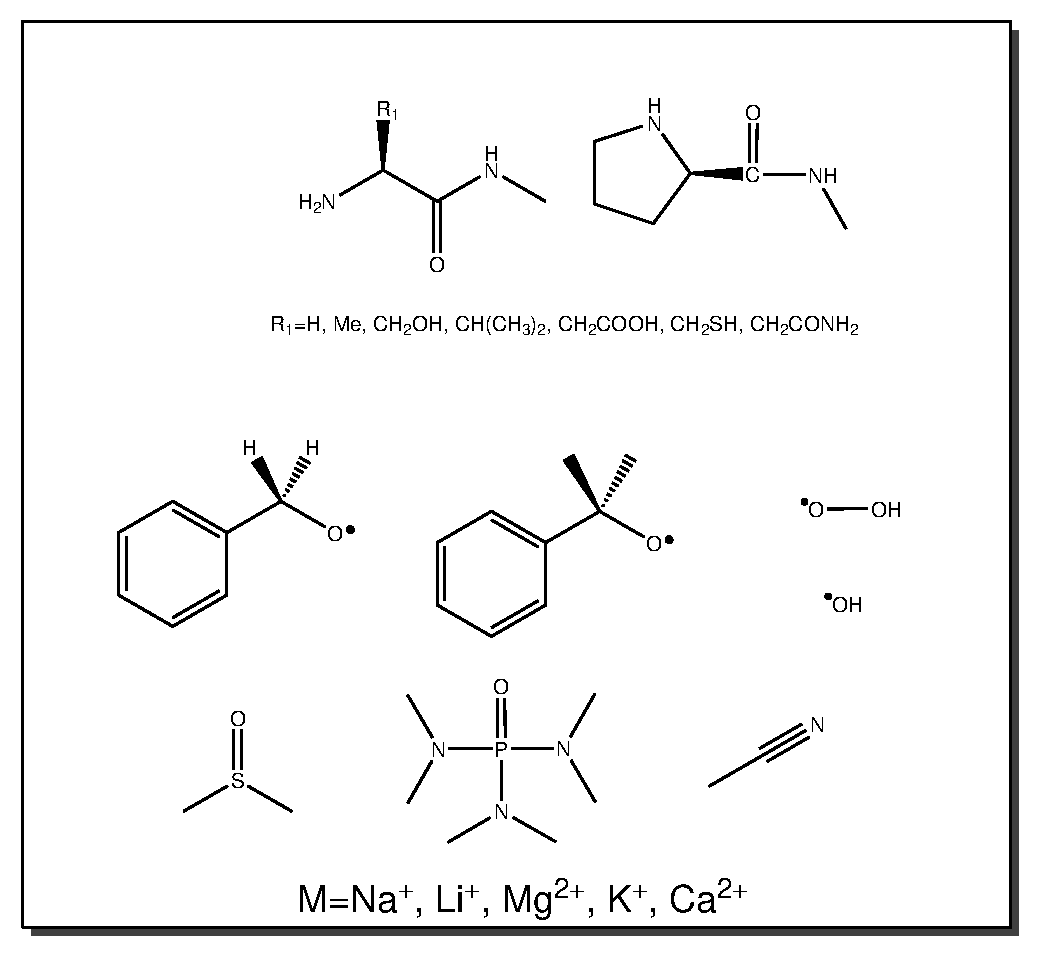
\includegraphics[width=\textwidth]{figures/set1.eps}
    \caption[Initial proposed benchmark set of substrates/radicals and metal cations.]{Initial proposed benchmark set of substrates/radicals and metal cations. Note this set consists of all combinations of substrates and metal cation, thus there are 75 complexes in the set. Conformational analysis using the Hyperchem package\cite{Hyperchem16} to identify the lowest energy conformers of all the substrates was completed using the AM1 semi-empirical approach. Geometry optimizations were then performed without metal cations at the LC-$\omega$PBE-D3(BJ)/6-31+G(2d,2p) level of theory. Several binding sites were investigated and optimized at the same level of theory. Benchmark quality structures have been optimized at the LC-$\omega$PBE-D3(BJ)/6-311+G(3df,3pd) level of theory. I am awaiting computational resources to performed CCSD(T)-F12$^*$/Def2-QZVPPD calculations.}
  \label{fig:ap-set1}
\end{scheme}

\begin{figure}[!htbp]
  \centering
    \includegraphics[width=\textwidth]{figures/ap_pes_metals}
    \caption[Basis set convergence for sodium and magnesium ions with core-correlation basis sets.]{Basis set convergence of CCSD(T,Full)/cc-pVC$X$Z ($X$=3,4,5) for sodium and magnesium ions. The relative energy of each basis set relative to the cc-pVCDZ for each metal. The cardinal number of the basis sets is $X$.}
  \label{fig:ap_pes_metals}
\end{figure}

\begin{figure}[!htbp]
  \centering
    \includegraphics[width=\textwidth]{figures/ap_metals_explicit}
    \caption[Explicitly correlated basis set convergence for alkali and alkaline earth-metal cations.]{Explicitly correlated CCSD(T,Full)-F12$^*$/Def2-$X$ ($X$=SVP,TZVPPD,QZVPPD) basis set convergence for alkali and alkaline earth-metal cations. The relative energy of each basis set relative to the Def2-SVP for each metal. The cardinal number of the basis sets is $X$.}
  \label{fig:ap_metals_explicit}
\end{figure}


\end{document}
\endinput
